\section{Exploiting the Signal}

As discussed in Section
\ref{sec:data:char},
there are several predictable characteristics among reads which can be exploited
to gain more compression.
We have already used statistical information about the zig-zag deltas to our
advantage in the vbbe21 encoding (Section \ref{sec:vbbe21}) but we can even
further exploit the signal's characteristics by intimately tying this knowledge
to a compression algorithm. This understanding should improve the compression
ratio since compression is fundamentally an artificial intelligence problem of
understanding and prediction.

\subsubsection{Subsequence Searching}
Some of the previously discussed compression methods, such as bit packing and FOR, depend on global statistics of the data such as the minimum and maximum.
For nanopore signal data, these statistics are easily dominated by outliers in the data.
One naive solution is to separately compress adjacent subsequences of equal length.
This approach has previously been successful in the literature with methods such as SIMD-BP128 and fast patched frame-of-reference (FastPFOR) performing compression in blocks of 128 integers \cite{lemire-simd}.

% Explore blocks of different sizes
% Explore blocks of different equal splits

Consider partitioning the nanopore signal into adjacent variable length blocks.
Let $P(x,s)$ be the partitioning of signal $x$ into $|s|=m\ge 1$ partitions according to partitioner $s$ where
\[ s := (s_j \in \mathbb{Z}\cap [0, n) \mid s_0 = 0)\]
and $s_j$ is the starting index of the $j$-th partition such that
\[ P(x,s) = (p_j) := ((x_{s_j},x_{s_j+1},\dots,x_{s_{j+1}-1}))_{j\in\mathbb{Z}\cap[0,m)}.\]
% TODO this is not correct for the last partition
%((x_{s_0},x_{s_0+1},\dots,x_{s_1-1}),(x_{s_1},\dots,x_{s_2-1}),\dots,(x_{s_{m-1}},\dots,x_n)) .\]
For example, if $x=(656,527,515,527,526)$ and $s = (0,3,4)$ then $m=3$ and
\[P(x,s)=((656,527,515),(527),(526)).\]

Given the partitioning $P$ we would like to compress each partition $p_j$ separately and concatenate the results.
Let $M(p)$ be the compressed bytes of partition $p$ after applying compression method $M$.
Then, the compressed bytes of signal $x$ under partitioner $s$ is the concatenation of the compressed bytes of each partition $M(p_j)$ given by
\[ C(x,s,M) := (M(p_j)\mid p_j=P(x,s)_j). \]
Let $\hat s$ be the partitioner of $x$ which minimises the number of compressed bytes
\[ |C(x,\hat s,M)| = \min_s |C(x,s,M)| = \min_s \sum_j|M(p_j)|. \]
The minimum number of compressed bytes can be found using the following recursive relationship
\begin{align*}
	|C(x,\hat s,M)| &= M(x) & n = 1\\
	|C(x,\hat s,M)| &= \min\{M(x),\min_{0\le k\le n-2}\{|C(x_L,\hat s_{x_L},M)| + |C(x_R,\hat s_{x_R},M)|\}\} & n\ge 2
\end{align*}
where $x_L=(x_0,x_1,\dots,x_k)$ and $x_R=(x_{k+1},\dots,x_{n-1})$.
That is, the compressed bytes with minimum length are found by either compressing the whole signal as usual or by dividing the signal into two partitions and concatenating each partition's minimum length compressed bytes.

For a signal of size $n$, the number of comparisons is given by the recurrence relation
\begin{align*}
	c_1 &= c_{M,1}\\
	c_n &= c_{M,n} + \sum_{k=0}^{n-2}(c_{k+1}+c_{n-k-1} + 1) &n\ge 2
	%TODO +1 for adding?
\end{align*}
where $c_{M,n}$ is the number of comparisons for the compression method $M$ on input size $n$.
This can be simplified as follows
\begin{align*}
	c_n &= c_{M,n} + \sum_{k=1}^{n-1}(2c_k + 1)\\
	&= c_{M,n} + n-1 + 2\sum_{k=1}^{n-1}c_k &n\ge 2
\end{align*}
Let's write $c_n$ in terms of $c_{n-1}$ in order to solve the recurrence more easily.
\begin{align*}
	c_{n-1} &= c_{M,n-1} + n - 2 + 2\sum_{k=1}^{n-2}c_k & n\ge 3\\
	c_{n} - c_{n-1} &= c_{M,n} - c_{M,n-1} + 1 + 2c_{n-1} \\
	c_{n} &= c_{M,n} - c_{M,n-1} + 1 + 3c_{n-1} & n\ge 2
\end{align*}
%TODO cite formula here?
Unrolling this we find that
\begin{align*}
	c_n &= c_{M,n} + \sum_{k=1}^{n-1}3^{k-1}(2c_{M,n-k} + 1) & n\ge 2.
\end{align*}
If the compression method has linear time complexity (i.e. $c_{M,n} = O(n)$) then
\begin{align*}
	c_n &= O(n) + \sum_{k=1}^{n-1}3^{k-1}(2O(n-k) + 1)\\
	&= O(n) + \sum_{k=1}^{n-1}3^{k-1}O(n-k)\\
	&= O(3^n) & \text{See Appendix \ref{app:cn}}
\end{align*}
That is, it takes exponential time to find the minimum compressed size using the naive recursive algorithm.
%TODO why different to subsequence sum

However, this algorithm re-computes the compressed bytes of subsequences many times rather than calculating it once and caching the data.
A better approach is to use bottom-up dynamic programming which avoids recursion and hence stack overflows.
The approach would compute the minimum number of compressed bytes for all subsequences of length $1$ then $2$, $3$ and so forth up to $n$. The results are stored in a triangular matrix $OPT\in \mathbb{N}\times\mathbb{N}$ where $OPT_{i,j}$ is the minimum number of compressed bytes of the subsequence starting at index $i$ and ending at index $j$.
It is triangular since we are not interested in subsequences which end before they begin. That is, we require that $i\le j$.

%TODO put algorithm here

For a signal of size $n$, the algorithm has the following number of comparisons
\[ \tilde c_n = \sum_{k=1}^n(n-k+1)(c_{M,k}+k-1) \]
since there are $n-k+1$ subsequences of size $k$ and each must compare compressing itself to concatenating $k-1$ pairs of compressed subdivisions.
Suppose as before that the compression method takes linear time. Then $\tilde c_n$ simplifies to
\begin{align*}
	\tilde c_n &= \sum_{k=1}^n(n-k+1)(O(k)+k-1)\\
	&= \sum_{k=1}^n(n-k+1)O(k)\\
	&= O(n^3) &\text{See Appendix \ref{app:cn-dyn}}
\end{align*}
Interestingly, $c_n$ and $\tilde c_n$ are asymptotically related by having opposite base and power terms; 3 and $n$.

%What is the length of these subsequences?

We can speed up the algorithm without a significant loss in compression by ignoring subsequences smaller than $l$ and moving between subsequence lengths at a step of $\delta_1$ and subsequences of the same length at a step of $\delta_2$.
The idea is that for compression method $M$, there exists some $l$ such that the minimum number of compressed bytes of subsequence $y$ with size $|y|<l$ equals the number of regular compressed bytes of $y$ with high probability.
In mathematical notation $\exists l\in\mathbb{N}^+$ such that $\forall x,\;|x|<l$
\[ P(C(x,\hat s,M)=M(x))> 1-\epsilon\]
for small $\epsilon \le 0.05$.
Furthermore, it is not necessary to calculate subsequences of all lengths or all subsequences of the same length since subsequences which differ by a couple signals should not provide a significantly better partition. This is because the deltas between successive signal values are small.
Rather, we want to calculate the minimum number of compressed bytes for subsequences of length $l,l+\delta_1,l+2\delta_1,\dots,l + \lfloor\frac{n-l}{\delta_1}\rfloor\delta_1, n$.
Then for subsequences of a particular length $p$ we calculate the minimum number of compressed bytes for subsequences $\delta_2$ apart, of the form $(x_{i\delta_2},x_{1+i\delta_2},\dots,x_{p-1+ i\delta_2})$ where $0\le i\le \lfloor \frac{n-p}{\delta_2} \rfloor$.

%TODO put algorithm here

For a signal of size $n$, the algorithm now has the following number of comparisons
%\[ \tilde c_n = \sum_{k=l}^n(n-k+1)(c_{M,k}+k-1) \]

However, we can exploit the characteristics of nanopore signal data to find better subsequences.
For example, each read typically consists of a stall.

%The next idea is to divide $x$ into subsequences with small range and compress each subsequence separately.
%Let $OPT(i, j)$ be the minimum number of bytes after compressing $(x_i,\dots, x_j)$. Then,
%\[ OPT(i, j) = \min(bytes(i, j),\min_{i\le k<j}(OPT(i, k) + OPT(k+1, j))) \]


\subsection{The Stall}

\subsection{The Stall}

\subsection{The Stall}

\subsection{The Stall}

\input{plots/stall}

We will now explore stall-specific compression strategies.
Recall that the stall is the section of a read which occurs at
the beginning between the surge and pre-adapter surge. See Figure
\ref{fig:start-sections} for some context and Figure \ref{fig:stall} for a
close-up of the section. It is thought to occur due to the motor protein `stalling'
before it begins to unwind the molecule through the nanopore. It consists of
hundreds to thousands of data points which oscillate with little variation
around the read's median. The stall is a highly likely occurrence in any read,
for instance, only 6 reads in the data set do not have a stall.
However, its length varies from read to read, ranging from 34 to \num{37128}
with a mean of 1140.33. See Table \ref{tab:stall-n} for more information.

\input{plots/stall-n-tab}

Since this section oscillates with little variance around the read's median,
the maximum and minimum are much closer than in the DNA section.
Notably, the standard deviation of raw signal values in a stall is 5.72 compared
to 35.07 for the whole data set.
Instead of computing the zig-zag deltas we could transform the stall by subtract
its minimum point from all other stall points (FOR encoding) then
apply a suitable compression algorithm such as range coding. The idea is that
this could create a distribution with a lower entropy than the stall's zig-zag
deltas and hence more potential for compression.

Now we will define this strategy more formally. The \textit{stall} encoding
stores the stall's starting index (2 bytes), length (2 bytes), compressed size
(2 bytes) and compressed data (variable bytes) followed by the non-stall's
compressed size (4 bytes) and compressed data (variable bytes). The stall is
compressed using a \textit{stall-specific} encoding, whilst the non-stall is
compressed using a \textit{generic} algorithm.  See Figure \ref{fig:stall-enc}.
This method is more space-advantageous if
\[ C_{stall}(r) < C_{generic}(r) \]
where
\[ C_{stall}(r) = C_{specific}(r_s) + C_{generic}(r\setminus r_s) + 10. \]
In the above equations, $r\in\Omega$ is a read from the space of possible reads and $r_s$ is the
read's stall section. That is, this method is advantageous if its total
compressed size, consisting of the compressed stall, the compressed non-stall
and 10 bytes of metadata, is less than the usual encoding.

\input{plots/stall-enc}

The encoding could dynamically make the above comparison to decide
whether the stall is worth encoding or not. Then it could store an extra bit (or
byte for convenience) to flag whether the stall or generic algorithm is being
used. Let's name this algorithm the \textit{dynamic stall} encoding or
\textit{dstall} for short. See Figure \ref{fig:dstall-enc}. However, this extra
byte is a waste of space if the large majority of reads benefit from separate
stall encoding.

\input{plots/dstall-enc}

Consider our stall-specific encoding to be the FOR encoding followed by the
regular vbbe21 encoding (vbbe21) and range coding (altogether
\textit{rc-vbbe21-for}). Furthermore, let the generic algorithm be the
vbbe21-zd encoding followed by range coding (altogether
\textit{rc-vbbe21-zd}).
We shall name the stall encoding which uses the stall-specific encoding
rc-vbbe21-for and the generic encoding rc-vbbe21-zd: \textit{stall-fz}.
Similarly, we shall name \textit{dstall-fz} the dstall encoding which uses the
same stall-specific and generic encodings as stall-fz.

The compression ratio of stall-fz outperforms the generic method rc-vbbe21-zd
more often than not on reads with stalls of length greater than or equal to
1500. See Figure
\ref{fig:stall-best}. This means we could simply choose to encode the stall
separately when its length is at least 1500. Let's name this strategy
\textit{dstall-fz-1500}. Since most stalls are smaller than
1500 in size let's store an extra byte at the beginning of the encoding to flag
whether the stall is being encoded or not. If not, the stall specific section is
not recorded at all. This is equivalent to the dstall encoding in Figure
\ref{fig:dstall-enc} with the exception of how the stall encoding decision is
made. The advantage is that the read only needs to be compressed once rather
than twice as in the dstall algorithm. This is because dstall must compare
compressing the stall separately to not and so must check both ways before
proceeding. On the other hand, the dstall-fz-1500 strategy approximates the
dstall-fz decision boundary and hence should be faster during compression with
no speed difference during decompression. The compression ratio of
dstall-fz-1500 will not be better than dstall-fz but there should be little
difference if the decision boundary approximation is good.

%\input{plots/stall-ratio}
\input{plots/stall-best}


We will now explore stall-specific compression strategies.
Recall that the stall is the section of a read which occurs at
the beginning between the surge and pre-adapter surge. See Figure
\ref{fig:start-sections} for some context and Figure \ref{fig:stall} for a
close-up of the section. It is thought to occur due to the motor protein `stalling'
before it begins to unwind the molecule through the nanopore. It consists of
hundreds to thousands of data points which oscillate with little variation
around the read's median. The stall is a highly likely occurrence in any read,
for instance, only 6 reads in the data set do not have a stall.
However, its length varies from read to read, ranging from 34 to \num{37128}
with a mean of 1140.33. See Table \ref{tab:stall-n} for more information.

\begin{table}
    \caption{\label{tab:stall-n} Summary statistics of the data's stall lengths.}
    \begin{tabular}{|l|l|}
        \hline
Min & 34\\
	    Q1 & 314\\

Q2 & 771\\
	    Q3 & 1156\\
Max & 37128\\
\hline
Mean & 1140.33\\
	    Mode & 39\\
Sample SD & 1214.781\\
	\hline
    \end{tabular}
\end{table}


Since this section oscillates with little variance around the read's median,
the maximum and minimum are much closer than in the DNA section.
Notably, the standard deviation of raw signal values in a stall is 5.72 compared
to 35.07 for the whole data set.
Instead of computing the zig-zag deltas we could transform the stall by subtract
its minimum point from all other stall points (FOR encoding) then
apply a suitable compression algorithm such as range coding. The idea is that
this could create a distribution with a lower entropy than the stall's zig-zag
deltas and hence more potential for compression.

Now we will define this strategy more formally. The \textit{stall} encoding
stores the stall's starting index (2 bytes), length (2 bytes), compressed size
(2 bytes) and compressed data (variable bytes) followed by the non-stall's
compressed size (4 bytes) and compressed data (variable bytes). The stall is
compressed using a \textit{stall-specific} encoding, whilst the non-stall is
compressed using a \textit{generic} algorithm.  See Figure \ref{fig:stall-enc}.
This method is more space-advantageous if
\[ C_{stall}(r) < C_{generic}(r) \]
where
\[ C_{stall}(r) = C_{specific}(r_s) + C_{generic}(r\setminus r_s) + 10. \]
In the above equations, $r\in\Omega$ is a read from the space of possible reads and $r_s$ is the
read's stall section. That is, this method is advantageous if its total
compressed size, consisting of the compressed stall, the compressed non-stall
and 10 bytes of metadata, is less than the usual encoding.

\begin{figure}
\centering\begin{tikzpicture}[node distance=0cm,start chain=1 going right,start chain=2 going right] \footnotesize
  \tikzstyle{mytape}=[draw,minimum height=1.5cm]
	\node(A1)  [on chain=1,mytape,fill=yellow!20] {$\underbrace{\overbracket{\text{ }p\text{ }}^{\text{2 bytes}}}_{\text{stall start position}}$};
	\node(A2)  [on chain=1,mytape,fill=yellow!20] {$\underbrace{\overbracket{|r_s|}^{\text{2 bytes}}}_{\text{stall length}}$};
	\node(A3)  [on chain=1,mytape,fill=yellow!20] {$\underbrace{\overbracket{m_s}^{\text{2 bytes}}}_{\text{stall compressed size}}$};
	\node(A4)  [on chain=1,mytape,fill=green!20] {$\underbrace{\overbracket{C_{specific}(r_s)}^{m_s\text{ bytes}}}_{\text{stall compressed data}}$};
	\node(B1)  [on chain=1,mytape,fill=yellow!35] {$\underbrace{\overbracket{m}^{\text{4 bytes}}}_{\text{non-stall compressed size}}$};
	\node(B2)  [on chain=1,mytape,fill=green!35] {$\underbrace{\overbracket{C_{generic}(r\setminus r_s)}^{m\text{ bytes}}}_{\text{non-stall compressed data}}$};
\end{tikzpicture}
	\caption{\label{fig:stall-enc}The stall encoding records the stall's
starting position in the read, length, compressed size and compressed data,
	followed by the non-stall's compressed size and compressed data.
	The specific and generic compression algorithms used are known
	beforehand and hence are not stored. stall-fz uses rccm-vbbe21-for and
	rccm-vbbe21-zd as the specific and generic algorithm respectively.}
\end{figure}


The encoding could dynamically make the above comparison to decide
whether the stall is worth encoding or not. Then it could store an extra bit (or
byte for convenience) to flag whether the stall or generic algorithm is being
used. Let's name this algorithm the \textit{dynamic stall} encoding or
\textit{dstall} for short. See Figure \ref{fig:dstall-enc}. However, this extra
byte is a waste of space if the large majority of reads benefit from separate
stall encoding.

\usetikzlibrary{decorations.pathreplacing,positioning,calc}

\begin{figure}
\centering\begin{tikzpicture}[node distance=0cm,start chain=1 going right,start chain=2 going right] \footnotesize
  \tikzstyle{mytape}=[draw,minimum height=1.5cm]
	\node(A0)  [on chain=1,mytape,fill=blue!20] {$\underbrace{\overbracket{flag}^{\text{1 byte}}}_{\text{stall encoded flag}}$};
	\node(A1)  [on chain=1,mytape,fill=yellow!20] {$\underbrace{\overbracket{\text{ }p\text{ }}^{\text{2 bytes}}}_{\text{stall start position}}$};
	\node(A2)  [on chain=1,mytape,fill=yellow!20] {$\underbrace{\overbracket{|r_s|}^{\text{2 bytes}}}_{\text{stall length}}$};
	\node(A3)  [on chain=1,mytape,fill=yellow!20] {$\underbrace{\overbracket{m_s}^{\text{2 bytes}}}_{\text{stall compressed size}}$};
	\node(A4)  [on chain=1,mytape,fill=green!20] {$\underbrace{\overbracket{C_{specific}(r_s)}^{m_s\text{ bytes}}}_{\text{stall compressed data}}$};
	\node(B1)  [on chain=1,mytape,fill=yellow!35] {$\underbrace{\overbracket{m}^{\text{4 bytes}}}_{\text{non-stall compressed size}}$};
	\node(B2)  [on chain=1,mytape,fill=green!35] {$\underbrace{\overbracket{C_{generic}(r\setminus r_s)}^{m\text{ bytes}}}_{\text{non-stall compressed data}}$};
	\draw
	[decorate,decoration={brace,amplitude=5pt,mirror,raise=4ex}]
	  ($(A1)-(0,0.3)$) -- ($(A4)-(0,0.3)$) node[midway,yshift=-3em]{if $flag=1$};
\end{tikzpicture}
	\caption{\label{fig:dstall-enc}The dstall encoding stores an extra byte
	at the beginning to mark whether the stall is being encoded or not. If
	it is being encoded the remaining data matches the stall encoding.
	Otherwise, $r_s$ is empty and the whole read is compressed using the
	generic algorithm as usual. That is, the read's compressed size (4
	bytes) and data follows the flag.}
\end{figure}


Consider our stall-specific encoding to be the FOR encoding followed by the
regular vbbe21 encoding (vbbe21) and range coding (altogether
\textit{rc-vbbe21-for}). Furthermore, let the generic algorithm be the
vbbe21-zd encoding followed by range coding (altogether
\textit{rc-vbbe21-zd}).
We shall name the stall encoding which uses the stall-specific encoding
rc-vbbe21-for and the generic encoding rc-vbbe21-zd: \textit{stall-fz}.
Similarly, we shall name \textit{dstall-fz} the dstall encoding which uses the
same stall-specific and generic encodings as stall-fz.

The compression ratio of stall-fz outperforms the generic method rc-vbbe21-zd
more often than not on reads with stalls of length greater than or equal to
1500. See Figure
\ref{fig:stall-best}. This means we could simply choose to encode the stall
separately when its length is at least 1500. Let's name this strategy
\textit{dstall-fz-1500}. Since most stalls are smaller than
1500 in size let's store an extra byte at the beginning of the encoding to flag
whether the stall is being encoded or not. If not, the stall specific section is
not recorded at all. This is equivalent to the dstall encoding in Figure
\ref{fig:dstall-enc} with the exception of how the stall encoding decision is
made. The advantage is that the read only needs to be compressed once rather
than twice as in the dstall algorithm. This is because dstall must compare
compressing the stall separately to not and so must check both ways before
proceeding. On the other hand, the dstall-fz-1500 strategy approximates the
dstall-fz decision boundary and hence should be faster during compression with
no speed difference during decompression. The compression ratio of
dstall-fz-1500 will not be better than dstall-fz but there should be little
difference if the decision boundary approximation is good.

%\begin{figure}
\centering
\input{plots/reads.blow5.test.svbbe21.read.prop}
\caption{\label{fig:stall-ratio}The 100\% stacked histogram of the compression
	methods with the highest compression ratio for all the reads in the data
	versus their stall length. Reads with a stall length $\sim$1500 and
	greater are more likely to be compressed smaller using stall-fz than
	rc-vbbe21-zd.}
\end{figure}

\begin{figure}
\centering
%\input{plots/reads.blow5.test.svbbe21.read.best}
\includegraphics[scale=0.7]{plots/reads.blow5.test.svbbe21.read.update.best.pdf}
	\caption[A scatter plot of the compression methods with
the highest compression ratio on each read out of rc01s-vbbe21-zd and stall-fz.]{\label{fig:stall-best}A scatter plot of the compression methods with
the highest compression ratio on each read out of rc01s-vbbe21-zd and stall-fz. The
best compression ratio is plotted against the length of the read's stall. Reads
with a stall length $\sim$1500 and greater are more likely to be compressed
smaller with stall-fz rather than rc01s-vbbe21-zd.}
\end{figure}



We will now explore stall-specific compression strategies.
Recall that the stall is the section of a read which occurs at
the beginning between the surge and pre-adapter surge. See Figure
\ref{fig:start-sections} for some context and Figure \ref{fig:stall} for a
close-up of the section. It is thought to occur due to the motor protein `stalling'
before it begins to unwind the molecule through the nanopore. It consists of
hundreds to thousands of data points which oscillate with little variation
around the read's median. The stall is a highly likely occurrence in any read,
for instance, only 6 reads in the data set do not have a stall.
However, its length varies from read to read, ranging from 34 to \num{37128}
with a mean of 1140.33. See Table \ref{tab:stall-n} for more information.

\begin{table}
    \caption{\label{tab:stall-n} Summary statistics of the data's stall lengths.}
    \begin{tabular}{|l|l|}
        \hline
Min & 34\\
	    Q1 & 314\\

Q2 & 771\\
	    Q3 & 1156\\
Max & 37128\\
\hline
Mean & 1140.33\\
	    Mode & 39\\
Sample SD & 1214.781\\
	\hline
    \end{tabular}
\end{table}


Since this section oscillates with little variance around the read's median,
the maximum and minimum are much closer than in the DNA section.
Notably, the standard deviation of raw signal values in a stall is 5.72 compared
to 35.07 for the whole data set.
Instead of computing the zig-zag deltas we could transform the stall by subtract
its minimum point from all other stall points (FOR encoding) then
apply a suitable compression algorithm such as range coding. The idea is that
this could create a distribution with a lower entropy than the stall's zig-zag
deltas and hence more potential for compression.

Now we will define this strategy more formally. The \textit{stall} encoding
stores the stall's starting index (2 bytes), length (2 bytes), compressed size
(2 bytes) and compressed data (variable bytes) followed by the non-stall's
compressed size (4 bytes) and compressed data (variable bytes). The stall is
compressed using a \textit{stall-specific} encoding, whilst the non-stall is
compressed using a \textit{generic} algorithm.  See Figure \ref{fig:stall-enc}.
This method is more space-advantageous if
\[ C_{stall}(r) < C_{generic}(r) \]
where
\[ C_{stall}(r) = C_{specific}(r_s) + C_{generic}(r\setminus r_s) + 10. \]
In the above equations, $r\in\Omega$ is a read from the space of possible reads and $r_s$ is the
read's stall section. That is, this method is advantageous if its total
compressed size, consisting of the compressed stall, the compressed non-stall
and 10 bytes of metadata, is less than the usual encoding.

\begin{figure}
\centering\begin{tikzpicture}[node distance=0cm,start chain=1 going right,start chain=2 going right] \footnotesize
  \tikzstyle{mytape}=[draw,minimum height=1.5cm]
	\node(A1)  [on chain=1,mytape,fill=yellow!20] {$\underbrace{\overbracket{\text{ }p\text{ }}^{\text{2 bytes}}}_{\text{stall start position}}$};
	\node(A2)  [on chain=1,mytape,fill=yellow!20] {$\underbrace{\overbracket{|r_s|}^{\text{2 bytes}}}_{\text{stall length}}$};
	\node(A3)  [on chain=1,mytape,fill=yellow!20] {$\underbrace{\overbracket{m_s}^{\text{2 bytes}}}_{\text{stall compressed size}}$};
	\node(A4)  [on chain=1,mytape,fill=green!20] {$\underbrace{\overbracket{C_{specific}(r_s)}^{m_s\text{ bytes}}}_{\text{stall compressed data}}$};
	\node(B1)  [on chain=1,mytape,fill=yellow!35] {$\underbrace{\overbracket{m}^{\text{4 bytes}}}_{\text{non-stall compressed size}}$};
	\node(B2)  [on chain=1,mytape,fill=green!35] {$\underbrace{\overbracket{C_{generic}(r\setminus r_s)}^{m\text{ bytes}}}_{\text{non-stall compressed data}}$};
\end{tikzpicture}
	\caption{\label{fig:stall-enc}The stall encoding records the stall's
starting position in the read, length, compressed size and compressed data,
	followed by the non-stall's compressed size and compressed data.
	The specific and generic compression algorithms used are known
	beforehand and hence are not stored. stall-fz uses rccm-vbbe21-for and
	rccm-vbbe21-zd as the specific and generic algorithm respectively.}
\end{figure}


The encoding could dynamically make the above comparison to decide
whether the stall is worth encoding or not. Then it could store an extra bit (or
byte for convenience) to flag whether the stall or generic algorithm is being
used. Let's name this algorithm the \textit{dynamic stall} encoding or
\textit{dstall} for short. See Figure \ref{fig:dstall-enc}. However, this extra
byte is a waste of space if the large majority of reads benefit from separate
stall encoding.

\usetikzlibrary{decorations.pathreplacing,positioning,calc}

\begin{figure}
\centering\begin{tikzpicture}[node distance=0cm,start chain=1 going right,start chain=2 going right] \footnotesize
  \tikzstyle{mytape}=[draw,minimum height=1.5cm]
	\node(A0)  [on chain=1,mytape,fill=blue!20] {$\underbrace{\overbracket{flag}^{\text{1 byte}}}_{\text{stall encoded flag}}$};
	\node(A1)  [on chain=1,mytape,fill=yellow!20] {$\underbrace{\overbracket{\text{ }p\text{ }}^{\text{2 bytes}}}_{\text{stall start position}}$};
	\node(A2)  [on chain=1,mytape,fill=yellow!20] {$\underbrace{\overbracket{|r_s|}^{\text{2 bytes}}}_{\text{stall length}}$};
	\node(A3)  [on chain=1,mytape,fill=yellow!20] {$\underbrace{\overbracket{m_s}^{\text{2 bytes}}}_{\text{stall compressed size}}$};
	\node(A4)  [on chain=1,mytape,fill=green!20] {$\underbrace{\overbracket{C_{specific}(r_s)}^{m_s\text{ bytes}}}_{\text{stall compressed data}}$};
	\node(B1)  [on chain=1,mytape,fill=yellow!35] {$\underbrace{\overbracket{m}^{\text{4 bytes}}}_{\text{non-stall compressed size}}$};
	\node(B2)  [on chain=1,mytape,fill=green!35] {$\underbrace{\overbracket{C_{generic}(r\setminus r_s)}^{m\text{ bytes}}}_{\text{non-stall compressed data}}$};
	\draw
	[decorate,decoration={brace,amplitude=5pt,mirror,raise=4ex}]
	  ($(A1)-(0,0.3)$) -- ($(A4)-(0,0.3)$) node[midway,yshift=-3em]{if $flag=1$};
\end{tikzpicture}
	\caption{\label{fig:dstall-enc}The dstall encoding stores an extra byte
	at the beginning to mark whether the stall is being encoded or not. If
	it is being encoded the remaining data matches the stall encoding.
	Otherwise, $r_s$ is empty and the whole read is compressed using the
	generic algorithm as usual. That is, the read's compressed size (4
	bytes) and data follows the flag.}
\end{figure}


Consider our stall-specific encoding to be the FOR encoding followed by the
regular vbbe21 encoding (vbbe21) and range coding (altogether
\textit{rc-vbbe21-for}). Furthermore, let the generic algorithm be the
vbbe21-zd encoding followed by range coding (altogether
\textit{rc-vbbe21-zd}).
We shall name the stall encoding which uses the stall-specific encoding
rc-vbbe21-for and the generic encoding rc-vbbe21-zd: \textit{stall-fz}.
Similarly, we shall name \textit{dstall-fz} the dstall encoding which uses the
same stall-specific and generic encodings as stall-fz.

The compression ratio of stall-fz outperforms the generic method rc-vbbe21-zd
more often than not on reads with stalls of length greater than or equal to
1500. See Figure
\ref{fig:stall-best}. This means we could simply choose to encode the stall
separately when its length is at least 1500. Let's name this strategy
\textit{dstall-fz-1500}. Since most stalls are smaller than
1500 in size let's store an extra byte at the beginning of the encoding to flag
whether the stall is being encoded or not. If not, the stall specific section is
not recorded at all. This is equivalent to the dstall encoding in Figure
\ref{fig:dstall-enc} with the exception of how the stall encoding decision is
made. The advantage is that the read only needs to be compressed once rather
than twice as in the dstall algorithm. This is because dstall must compare
compressing the stall separately to not and so must check both ways before
proceeding. On the other hand, the dstall-fz-1500 strategy approximates the
dstall-fz decision boundary and hence should be faster during compression with
no speed difference during decompression. The compression ratio of
dstall-fz-1500 will not be better than dstall-fz but there should be little
difference if the decision boundary approximation is good.

%\begin{figure}
\centering
% Created by tikzDevice version 0.12.3.1 on 2022-10-21 15:39:01
% !TEX encoding = UTF-8 Unicode
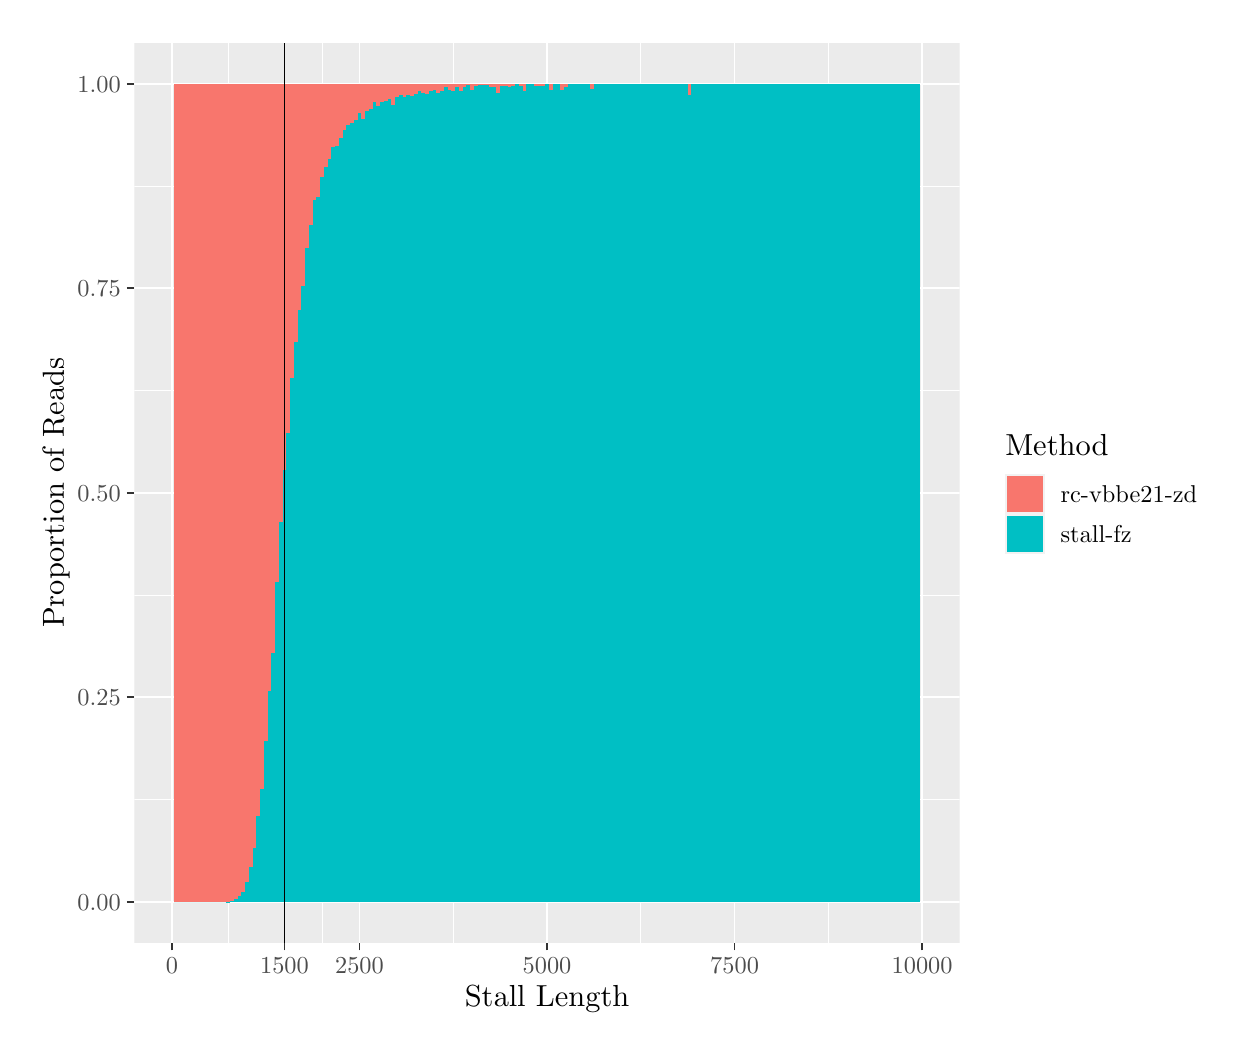
\begin{tikzpicture}[x=1pt,y=1pt]
\definecolor{fillColor}{RGB}{255,255,255}
\path[use as bounding box,fill=fillColor,fill opacity=0.00] (0,0) rectangle (433.62,361.35);
\begin{scope}
\path[clip] (  0.00,  0.00) rectangle (433.62,361.35);
\definecolor{drawColor}{RGB}{255,255,255}
\definecolor{fillColor}{RGB}{255,255,255}

\path[draw=drawColor,line width= 0.6pt,line join=round,line cap=round,fill=fillColor] (  0.00,  0.00) rectangle (433.62,361.35);
\end{scope}
\begin{scope}
\path[clip] ( 38.56, 30.69) rectangle (336.78,355.85);
\definecolor{fillColor}{gray}{0.92}

\path[fill=fillColor] ( 38.56, 30.69) rectangle (336.78,355.85);
\definecolor{drawColor}{RGB}{255,255,255}

\path[draw=drawColor,line width= 0.3pt,line join=round] ( 38.56, 82.42) --
	(336.78, 82.42);

\path[draw=drawColor,line width= 0.3pt,line join=round] ( 38.56,156.32) --
	(336.78,156.32);

\path[draw=drawColor,line width= 0.3pt,line join=round] ( 38.56,230.22) --
	(336.78,230.22);

\path[draw=drawColor,line width= 0.3pt,line join=round] ( 38.56,304.12) --
	(336.78,304.12);

\path[draw=drawColor,line width= 0.3pt,line join=round] ( 72.44, 30.69) --
	( 72.44,355.85);

\path[draw=drawColor,line width= 0.3pt,line join=round] (106.33, 30.69) --
	(106.33,355.85);

\path[draw=drawColor,line width= 0.3pt,line join=round] (153.78, 30.69) --
	(153.78,355.85);

\path[draw=drawColor,line width= 0.3pt,line join=round] (221.55, 30.69) --
	(221.55,355.85);

\path[draw=drawColor,line width= 0.3pt,line join=round] (289.33, 30.69) --
	(289.33,355.85);

\path[draw=drawColor,line width= 0.6pt,line join=round] ( 38.56, 45.47) --
	(336.78, 45.47);

\path[draw=drawColor,line width= 0.6pt,line join=round] ( 38.56,119.37) --
	(336.78,119.37);

\path[draw=drawColor,line width= 0.6pt,line join=round] ( 38.56,193.27) --
	(336.78,193.27);

\path[draw=drawColor,line width= 0.6pt,line join=round] ( 38.56,267.17) --
	(336.78,267.17);

\path[draw=drawColor,line width= 0.6pt,line join=round] ( 38.56,341.07) --
	(336.78,341.07);

\path[draw=drawColor,line width= 0.6pt,line join=round] ( 52.11, 30.69) --
	( 52.11,355.85);

\path[draw=drawColor,line width= 0.6pt,line join=round] ( 92.78, 30.69) --
	( 92.78,355.85);

\path[draw=drawColor,line width= 0.6pt,line join=round] (119.89, 30.69) --
	(119.89,355.85);

\path[draw=drawColor,line width= 0.6pt,line join=round] (187.67, 30.69) --
	(187.67,355.85);

\path[draw=drawColor,line width= 0.6pt,line join=round] (255.44, 30.69) --
	(255.44,355.85);

\path[draw=drawColor,line width= 0.6pt,line join=round] (323.22, 30.69) --
	(323.22,355.85);
\definecolor{fillColor}{RGB}{248,118,109}

\path[fill=fillColor] ( 52.79, 45.47) rectangle ( 54.14,341.07);

\path[fill=fillColor] ( 54.14, 45.47) rectangle ( 55.50,341.07);

\path[fill=fillColor] ( 55.50, 45.47) rectangle ( 56.85,341.07);

\path[fill=fillColor] ( 56.85, 45.47) rectangle ( 58.21,341.07);

\path[fill=fillColor] ( 58.21, 45.47) rectangle ( 59.57,341.07);

\path[fill=fillColor] ( 59.57, 45.47) rectangle ( 60.92,341.07);

\path[fill=fillColor] ( 60.92, 45.47) rectangle ( 62.28,341.07);

\path[fill=fillColor] ( 62.28, 45.47) rectangle ( 63.63,341.07);

\path[fill=fillColor] ( 63.63, 45.47) rectangle ( 64.99,341.07);

\path[fill=fillColor] ( 64.99, 45.47) rectangle ( 66.34,341.07);

\path[fill=fillColor] ( 66.34, 45.47) rectangle ( 67.70,341.07);

\path[fill=fillColor] ( 67.70, 45.47) rectangle ( 69.05,341.07);

\path[fill=fillColor] ( 69.05, 45.47) rectangle ( 70.41,341.07);

\path[fill=fillColor] ( 70.41, 45.47) rectangle ( 71.77,341.07);

\path[fill=fillColor] ( 71.77, 45.49) rectangle ( 73.12,341.07);

\path[fill=fillColor] ( 73.12, 45.92) rectangle ( 74.48,341.07);

\path[fill=fillColor] ( 74.48, 46.32) rectangle ( 75.83,341.07);

\path[fill=fillColor] ( 75.83, 47.48) rectangle ( 77.19,341.07);

\path[fill=fillColor] ( 77.19, 48.95) rectangle ( 78.54,341.07);

\path[fill=fillColor] ( 78.54, 52.57) rectangle ( 79.90,341.07);

\path[fill=fillColor] ( 79.90, 57.99) rectangle ( 81.25,341.07);

\path[fill=fillColor] ( 81.25, 64.89) rectangle ( 82.61,341.07);

\path[fill=fillColor] ( 82.61, 76.64) rectangle ( 83.97,341.07);

\path[fill=fillColor] ( 83.97, 86.37) rectangle ( 85.32,341.07);

\path[fill=fillColor] ( 85.32,103.73) rectangle ( 86.68,341.07);

\path[fill=fillColor] ( 86.68,121.80) rectangle ( 88.03,341.07);

\path[fill=fillColor] ( 88.03,135.40) rectangle ( 89.39,341.07);

\path[fill=fillColor] ( 89.39,161.09) rectangle ( 90.74,341.07);

\path[fill=fillColor] ( 90.74,182.61) rectangle ( 92.10,341.07);

\path[fill=fillColor] ( 92.10,201.69) rectangle ( 93.45,341.07);

\path[fill=fillColor] ( 93.45,214.83) rectangle ( 94.81,341.07);

\path[fill=fillColor] ( 94.81,234.71) rectangle ( 96.17,341.07);

\path[fill=fillColor] ( 96.17,247.88) rectangle ( 97.52,341.07);

\path[fill=fillColor] ( 97.52,259.33) rectangle ( 98.88,341.07);

\path[fill=fillColor] ( 98.88,268.04) rectangle (100.23,341.07);

\path[fill=fillColor] (100.23,281.77) rectangle (101.59,341.07);

\path[fill=fillColor] (101.59,290.15) rectangle (102.94,341.07);

\path[fill=fillColor] (102.94,299.08) rectangle (104.30,341.07);

\path[fill=fillColor] (104.30,300.06) rectangle (105.65,341.07);

\path[fill=fillColor] (105.65,307.56) rectangle (107.01,341.07);

\path[fill=fillColor] (107.01,310.83) rectangle (108.37,341.07);

\path[fill=fillColor] (108.37,313.71) rectangle (109.72,341.07);

\path[fill=fillColor] (109.72,318.32) rectangle (111.08,341.07);

\path[fill=fillColor] (111.08,318.61) rectangle (112.43,341.07);

\path[fill=fillColor] (112.43,321.62) rectangle (113.79,341.07);

\path[fill=fillColor] (113.79,324.46) rectangle (115.14,341.07);

\path[fill=fillColor] (115.14,326.00) rectangle (116.50,341.07);

\path[fill=fillColor] (116.50,326.99) rectangle (117.85,341.07);

\path[fill=fillColor] (117.85,328.11) rectangle (119.21,341.07);

\path[fill=fillColor] (119.21,330.49) rectangle (120.57,341.07);

\path[fill=fillColor] (120.57,328.48) rectangle (121.92,341.07);

\path[fill=fillColor] (121.92,331.26) rectangle (123.28,341.07);

\path[fill=fillColor] (123.28,331.80) rectangle (124.63,341.07);

\path[fill=fillColor] (124.63,334.52) rectangle (125.99,341.07);

\path[fill=fillColor] (125.99,333.20) rectangle (127.34,341.07);

\path[fill=fillColor] (127.34,334.33) rectangle (128.70,341.07);

\path[fill=fillColor] (128.70,334.88) rectangle (130.05,341.07);

\path[fill=fillColor] (130.05,335.69) rectangle (131.41,341.07);

\path[fill=fillColor] (131.41,333.30) rectangle (132.77,341.07);

\path[fill=fillColor] (132.77,336.15) rectangle (134.12,341.07);

\path[fill=fillColor] (134.12,336.96) rectangle (135.48,341.07);

\path[fill=fillColor] (135.48,336.47) rectangle (136.83,341.07);

\path[fill=fillColor] (136.83,337.17) rectangle (138.19,341.07);

\path[fill=fillColor] (138.19,336.65) rectangle (139.54,341.07);

\path[fill=fillColor] (139.54,337.46) rectangle (140.90,341.07);

\path[fill=fillColor] (140.90,338.46) rectangle (142.25,341.07);

\path[fill=fillColor] (142.25,337.85) rectangle (143.61,341.07);

\path[fill=fillColor] (143.61,337.32) rectangle (144.97,341.07);

\path[fill=fillColor] (144.97,338.55) rectangle (146.32,341.07);

\path[fill=fillColor] (146.32,338.66) rectangle (147.68,341.07);

\path[fill=fillColor] (147.68,337.90) rectangle (149.03,341.07);

\path[fill=fillColor] (149.03,338.44) rectangle (150.39,341.07);

\path[fill=fillColor] (150.39,339.75) rectangle (151.74,341.07);

\path[fill=fillColor] (151.74,338.93) rectangle (153.10,341.07);

\path[fill=fillColor] (153.10,338.63) rectangle (154.45,341.07);

\path[fill=fillColor] (154.45,339.91) rectangle (155.81,341.07);

\path[fill=fillColor] (155.81,338.52) rectangle (157.17,341.07);

\path[fill=fillColor] (157.17,339.80) rectangle (158.52,341.07);

\path[fill=fillColor] (158.52,340.63) rectangle (159.88,341.07);

\path[fill=fillColor] (159.88,338.85) rectangle (161.23,341.07);

\path[fill=fillColor] (161.23,340.14) rectangle (162.59,341.07);

\path[fill=fillColor] (162.59,340.59) rectangle (163.94,341.07);

\path[fill=fillColor] (163.94,340.58) rectangle (165.30,341.07);

\path[fill=fillColor] (165.30,340.53) rectangle (166.65,341.07);

\path[fill=fillColor] (166.65,339.91) rectangle (168.01,341.07);

\path[fill=fillColor] (168.01,339.95) rectangle (169.37,341.07);

\path[fill=fillColor] (169.37,337.56) rectangle (170.72,341.07);

\path[fill=fillColor] (170.72,340.42) rectangle (172.08,341.07);

\path[fill=fillColor] (172.08,340.40) rectangle (173.43,341.07);

\path[fill=fillColor] (173.43,339.76) rectangle (174.79,341.07);

\path[fill=fillColor] (174.79,340.31) rectangle (176.14,341.07);

\path[fill=fillColor] (176.14,341.07) rectangle (177.50,341.07);

\path[fill=fillColor] (177.50,340.29) rectangle (178.85,341.07);

\path[fill=fillColor] (178.85,338.62) rectangle (180.21,341.07);

\path[fill=fillColor] (180.21,341.07) rectangle (181.57,341.07);

\path[fill=fillColor] (181.57,341.07) rectangle (182.92,341.07);

\path[fill=fillColor] (182.92,340.22) rectangle (184.28,341.07);

\path[fill=fillColor] (184.28,340.23) rectangle (185.63,341.07);

\path[fill=fillColor] (185.63,340.17) rectangle (186.99,341.07);

\path[fill=fillColor] (186.99,341.07) rectangle (188.34,341.07);

\path[fill=fillColor] (188.34,338.90) rectangle (189.70,341.07);

\path[fill=fillColor] (189.70,341.07) rectangle (191.05,341.07);

\path[fill=fillColor] (191.05,341.07) rectangle (192.41,341.07);

\path[fill=fillColor] (192.41,338.74) rectangle (193.77,341.07);

\path[fill=fillColor] (193.77,339.77) rectangle (195.12,341.07);

\path[fill=fillColor] (195.12,341.07) rectangle (196.48,341.07);

\path[fill=fillColor] (196.48,341.07) rectangle (197.83,341.07);

\path[fill=fillColor] (197.83,341.07) rectangle (199.19,341.07);

\path[fill=fillColor] (199.19,341.07) rectangle (200.54,341.07);

\path[fill=fillColor] (200.54,341.07) rectangle (201.90,341.07);

\path[fill=fillColor] (201.90,341.07) rectangle (203.25,341.07);

\path[fill=fillColor] (203.25,339.32) rectangle (204.61,341.07);

\path[fill=fillColor] (204.61,341.07) rectangle (205.97,341.07);

\path[fill=fillColor] (205.97,341.07) rectangle (207.32,341.07);

\path[fill=fillColor] (207.32,341.07) rectangle (208.68,341.07);

\path[fill=fillColor] (208.68,341.07) rectangle (210.03,341.07);

\path[fill=fillColor] (210.03,341.07) rectangle (211.39,341.07);

\path[fill=fillColor] (211.39,341.07) rectangle (212.74,341.07);

\path[fill=fillColor] (212.74,341.07) rectangle (214.10,341.07);

\path[fill=fillColor] (214.10,341.07) rectangle (215.45,341.07);

\path[fill=fillColor] (215.45,341.07) rectangle (216.81,341.07);

\path[fill=fillColor] (216.81,341.07) rectangle (218.17,341.07);

\path[fill=fillColor] (218.17,341.07) rectangle (219.52,341.07);

\path[fill=fillColor] (219.52,341.07) rectangle (220.88,341.07);

\path[fill=fillColor] (220.88,341.07) rectangle (222.23,341.07);

\path[fill=fillColor] (222.23,341.07) rectangle (223.59,341.07);

\path[fill=fillColor] (223.59,341.07) rectangle (224.94,341.07);

\path[fill=fillColor] (224.94,341.07) rectangle (226.30,341.07);

\path[fill=fillColor] (226.30,341.07) rectangle (227.65,341.07);

\path[fill=fillColor] (227.65,341.07) rectangle (229.01,341.07);

\path[fill=fillColor] (229.01,341.07) rectangle (230.37,341.07);

\path[fill=fillColor] (230.37,341.07) rectangle (231.72,341.07);

\path[fill=fillColor] (231.72,341.07) rectangle (233.08,341.07);

\path[fill=fillColor] (233.08,341.07) rectangle (234.43,341.07);

\path[fill=fillColor] (234.43,341.07) rectangle (235.79,341.07);

\path[fill=fillColor] (235.79,341.07) rectangle (237.14,341.07);

\path[fill=fillColor] (237.14,341.07) rectangle (238.50,341.07);

\path[fill=fillColor] (238.50,337.13) rectangle (239.85,341.07);

\path[fill=fillColor] (239.85,341.07) rectangle (241.21,341.07);

\path[fill=fillColor] (241.21,341.07) rectangle (242.56,341.07);

\path[fill=fillColor] (242.56,341.07) rectangle (243.92,341.07);

\path[fill=fillColor] (243.92,341.07) rectangle (245.28,341.07);

\path[fill=fillColor] (245.28,341.07) rectangle (246.63,341.07);

\path[fill=fillColor] (246.63,341.07) rectangle (247.99,341.07);

\path[fill=fillColor] (247.99,341.07) rectangle (249.34,341.07);

\path[fill=fillColor] (249.34,341.07) rectangle (250.70,341.07);

\path[fill=fillColor] (250.70,341.07) rectangle (252.05,341.07);

\path[fill=fillColor] (252.05,341.07) rectangle (253.41,341.07);

\path[fill=fillColor] (253.41,341.07) rectangle (254.76,341.07);

\path[fill=fillColor] (254.76,341.07) rectangle (256.12,341.07);

\path[fill=fillColor] (256.12,341.07) rectangle (257.48,341.07);

\path[fill=fillColor] (257.48,341.07) rectangle (258.83,341.07);

\path[fill=fillColor] (258.83,341.07) rectangle (260.19,341.07);

\path[fill=fillColor] (260.19,341.07) rectangle (261.54,341.07);

\path[fill=fillColor] (261.54,341.07) rectangle (262.90,341.07);

\path[fill=fillColor] (262.90,341.07) rectangle (264.25,341.07);

\path[fill=fillColor] (264.25,341.07) rectangle (265.61,341.07);

\path[fill=fillColor] (265.61,341.07) rectangle (266.96,341.07);

\path[fill=fillColor] (266.96,341.07) rectangle (268.32,341.07);

\path[fill=fillColor] (268.32,341.07) rectangle (269.68,341.07);

\path[fill=fillColor] (269.68,341.07) rectangle (271.03,341.07);

\path[fill=fillColor] (271.03,341.07) rectangle (272.39,341.07);

\path[fill=fillColor] (272.39,341.07) rectangle (273.74,341.07);

\path[fill=fillColor] (273.74,341.07) rectangle (275.10,341.07);

\path[fill=fillColor] (275.10,341.07) rectangle (276.45,341.07);

\path[fill=fillColor] (276.45,341.07) rectangle (277.81,341.07);

\path[fill=fillColor] (277.81,341.07) rectangle (279.16,341.07);

\path[fill=fillColor] (279.16,341.07) rectangle (280.52,341.07);

\path[fill=fillColor] (280.52,341.07) rectangle (281.88,341.07);

\path[fill=fillColor] (281.88,341.07) rectangle (283.23,341.07);

\path[fill=fillColor] (283.23,341.07) rectangle (284.59,341.07);

\path[fill=fillColor] (284.59,341.07) rectangle (285.94,341.07);

\path[fill=fillColor] (285.94,341.07) rectangle (287.30,341.07);

\path[fill=fillColor] (287.30,341.07) rectangle (288.65,341.07);

\path[fill=fillColor] (288.65,341.07) rectangle (290.01,341.07);

\path[fill=fillColor] (290.01,341.07) rectangle (291.36,341.07);

\path[fill=fillColor] (291.36,341.07) rectangle (292.72,341.07);

\path[fill=fillColor] (292.72,341.07) rectangle (294.08,341.07);

\path[fill=fillColor] (294.08,341.07) rectangle (295.43,341.07);

\path[fill=fillColor] (295.43,341.07) rectangle (296.79,341.07);

\path[fill=fillColor] (296.79,341.07) rectangle (298.14,341.07);

\path[fill=fillColor] (298.14,341.07) rectangle (299.50,341.07);

\path[fill=fillColor] (299.50,341.07) rectangle (300.85,341.07);

\path[fill=fillColor] (300.85,341.07) rectangle (302.21,341.07);

\path[fill=fillColor] (302.21,341.07) rectangle (303.56,341.07);

\path[fill=fillColor] (303.56,341.07) rectangle (304.92,341.07);

\path[fill=fillColor] (304.92,341.07) rectangle (306.28,341.07);

\path[fill=fillColor] (306.28,341.07) rectangle (307.63,341.07);

\path[fill=fillColor] (307.63,341.07) rectangle (308.99,341.07);

\path[fill=fillColor] (308.99,341.07) rectangle (310.34,341.07);

\path[fill=fillColor] (310.34,341.07) rectangle (311.70,341.07);

\path[fill=fillColor] (311.70,341.07) rectangle (313.05,341.07);

\path[fill=fillColor] (313.05,341.07) rectangle (314.41,341.07);

\path[fill=fillColor] (314.41,341.07) rectangle (315.76,341.07);

\path[fill=fillColor] (315.76,341.07) rectangle (317.12,341.07);

\path[fill=fillColor] (317.12,341.07) rectangle (318.48,341.07);

\path[fill=fillColor] (318.48,341.07) rectangle (319.83,341.07);

\path[fill=fillColor] (319.83,341.07) rectangle (321.19,341.07);

\path[fill=fillColor] (321.19,341.07) rectangle (322.54,341.07);
\definecolor{fillColor}{RGB}{0,191,196}

\path[fill=fillColor] ( 52.79, 45.47) rectangle ( 54.14, 45.47);

\path[fill=fillColor] ( 54.14, 45.47) rectangle ( 55.50, 45.47);

\path[fill=fillColor] ( 55.50, 45.47) rectangle ( 56.85, 45.47);

\path[fill=fillColor] ( 56.85, 45.47) rectangle ( 58.21, 45.47);

\path[fill=fillColor] ( 58.21, 45.47) rectangle ( 59.57, 45.47);

\path[fill=fillColor] ( 59.57, 45.47) rectangle ( 60.92, 45.47);

\path[fill=fillColor] ( 60.92, 45.47) rectangle ( 62.28, 45.47);

\path[fill=fillColor] ( 62.28, 45.47) rectangle ( 63.63, 45.47);

\path[fill=fillColor] ( 63.63, 45.47) rectangle ( 64.99, 45.47);

\path[fill=fillColor] ( 64.99, 45.47) rectangle ( 66.34, 45.47);

\path[fill=fillColor] ( 66.34, 45.47) rectangle ( 67.70, 45.47);

\path[fill=fillColor] ( 67.70, 45.47) rectangle ( 69.05, 45.47);

\path[fill=fillColor] ( 69.05, 45.47) rectangle ( 70.41, 45.47);

\path[fill=fillColor] ( 70.41, 45.47) rectangle ( 71.77, 45.47);

\path[fill=fillColor] ( 71.77, 45.47) rectangle ( 73.12, 45.49);

\path[fill=fillColor] ( 73.12, 45.47) rectangle ( 74.48, 45.92);

\path[fill=fillColor] ( 74.48, 45.47) rectangle ( 75.83, 46.32);

\path[fill=fillColor] ( 75.83, 45.47) rectangle ( 77.19, 47.48);

\path[fill=fillColor] ( 77.19, 45.47) rectangle ( 78.54, 48.95);

\path[fill=fillColor] ( 78.54, 45.47) rectangle ( 79.90, 52.57);

\path[fill=fillColor] ( 79.90, 45.47) rectangle ( 81.25, 57.99);

\path[fill=fillColor] ( 81.25, 45.47) rectangle ( 82.61, 64.89);

\path[fill=fillColor] ( 82.61, 45.47) rectangle ( 83.97, 76.64);

\path[fill=fillColor] ( 83.97, 45.47) rectangle ( 85.32, 86.37);

\path[fill=fillColor] ( 85.32, 45.47) rectangle ( 86.68,103.73);

\path[fill=fillColor] ( 86.68, 45.47) rectangle ( 88.03,121.80);

\path[fill=fillColor] ( 88.03, 45.47) rectangle ( 89.39,135.40);

\path[fill=fillColor] ( 89.39, 45.47) rectangle ( 90.74,161.09);

\path[fill=fillColor] ( 90.74, 45.47) rectangle ( 92.10,182.61);

\path[fill=fillColor] ( 92.10, 45.47) rectangle ( 93.45,201.69);

\path[fill=fillColor] ( 93.45, 45.47) rectangle ( 94.81,214.83);

\path[fill=fillColor] ( 94.81, 45.47) rectangle ( 96.17,234.71);

\path[fill=fillColor] ( 96.17, 45.47) rectangle ( 97.52,247.88);

\path[fill=fillColor] ( 97.52, 45.47) rectangle ( 98.88,259.33);

\path[fill=fillColor] ( 98.88, 45.47) rectangle (100.23,268.04);

\path[fill=fillColor] (100.23, 45.47) rectangle (101.59,281.77);

\path[fill=fillColor] (101.59, 45.47) rectangle (102.94,290.15);

\path[fill=fillColor] (102.94, 45.47) rectangle (104.30,299.08);

\path[fill=fillColor] (104.30, 45.47) rectangle (105.65,300.06);

\path[fill=fillColor] (105.65, 45.47) rectangle (107.01,307.56);

\path[fill=fillColor] (107.01, 45.47) rectangle (108.37,310.83);

\path[fill=fillColor] (108.37, 45.47) rectangle (109.72,313.71);

\path[fill=fillColor] (109.72, 45.47) rectangle (111.08,318.32);

\path[fill=fillColor] (111.08, 45.47) rectangle (112.43,318.61);

\path[fill=fillColor] (112.43, 45.47) rectangle (113.79,321.62);

\path[fill=fillColor] (113.79, 45.47) rectangle (115.14,324.46);

\path[fill=fillColor] (115.14, 45.47) rectangle (116.50,326.00);

\path[fill=fillColor] (116.50, 45.47) rectangle (117.85,326.99);

\path[fill=fillColor] (117.85, 45.47) rectangle (119.21,328.11);

\path[fill=fillColor] (119.21, 45.47) rectangle (120.57,330.49);

\path[fill=fillColor] (120.57, 45.47) rectangle (121.92,328.48);

\path[fill=fillColor] (121.92, 45.47) rectangle (123.28,331.26);

\path[fill=fillColor] (123.28, 45.47) rectangle (124.63,331.80);

\path[fill=fillColor] (124.63, 45.47) rectangle (125.99,334.52);

\path[fill=fillColor] (125.99, 45.47) rectangle (127.34,333.20);

\path[fill=fillColor] (127.34, 45.47) rectangle (128.70,334.33);

\path[fill=fillColor] (128.70, 45.47) rectangle (130.05,334.88);

\path[fill=fillColor] (130.05, 45.47) rectangle (131.41,335.69);

\path[fill=fillColor] (131.41, 45.47) rectangle (132.77,333.30);

\path[fill=fillColor] (132.77, 45.47) rectangle (134.12,336.15);

\path[fill=fillColor] (134.12, 45.47) rectangle (135.48,336.96);

\path[fill=fillColor] (135.48, 45.47) rectangle (136.83,336.47);

\path[fill=fillColor] (136.83, 45.47) rectangle (138.19,337.17);

\path[fill=fillColor] (138.19, 45.47) rectangle (139.54,336.65);

\path[fill=fillColor] (139.54, 45.47) rectangle (140.90,337.46);

\path[fill=fillColor] (140.90, 45.47) rectangle (142.25,338.46);

\path[fill=fillColor] (142.25, 45.47) rectangle (143.61,337.85);

\path[fill=fillColor] (143.61, 45.47) rectangle (144.97,337.32);

\path[fill=fillColor] (144.97, 45.47) rectangle (146.32,338.55);

\path[fill=fillColor] (146.32, 45.47) rectangle (147.68,338.66);

\path[fill=fillColor] (147.68, 45.47) rectangle (149.03,337.90);

\path[fill=fillColor] (149.03, 45.47) rectangle (150.39,338.44);

\path[fill=fillColor] (150.39, 45.47) rectangle (151.74,339.75);

\path[fill=fillColor] (151.74, 45.47) rectangle (153.10,338.93);

\path[fill=fillColor] (153.10, 45.47) rectangle (154.45,338.63);

\path[fill=fillColor] (154.45, 45.47) rectangle (155.81,339.91);

\path[fill=fillColor] (155.81, 45.47) rectangle (157.17,338.52);

\path[fill=fillColor] (157.17, 45.47) rectangle (158.52,339.80);

\path[fill=fillColor] (158.52, 45.47) rectangle (159.88,340.63);

\path[fill=fillColor] (159.88, 45.47) rectangle (161.23,338.85);

\path[fill=fillColor] (161.23, 45.47) rectangle (162.59,340.14);

\path[fill=fillColor] (162.59, 45.47) rectangle (163.94,340.59);

\path[fill=fillColor] (163.94, 45.47) rectangle (165.30,340.58);

\path[fill=fillColor] (165.30, 45.47) rectangle (166.65,340.53);

\path[fill=fillColor] (166.65, 45.47) rectangle (168.01,339.91);

\path[fill=fillColor] (168.01, 45.47) rectangle (169.37,339.95);

\path[fill=fillColor] (169.37, 45.47) rectangle (170.72,337.56);

\path[fill=fillColor] (170.72, 45.47) rectangle (172.08,340.42);

\path[fill=fillColor] (172.08, 45.47) rectangle (173.43,340.40);

\path[fill=fillColor] (173.43, 45.47) rectangle (174.79,339.76);

\path[fill=fillColor] (174.79, 45.47) rectangle (176.14,340.31);

\path[fill=fillColor] (176.14, 45.47) rectangle (177.50,341.07);

\path[fill=fillColor] (177.50, 45.47) rectangle (178.85,340.29);

\path[fill=fillColor] (178.85, 45.47) rectangle (180.21,338.62);

\path[fill=fillColor] (180.21, 45.47) rectangle (181.57,341.07);

\path[fill=fillColor] (181.57, 45.47) rectangle (182.92,341.07);

\path[fill=fillColor] (182.92, 45.47) rectangle (184.28,340.22);

\path[fill=fillColor] (184.28, 45.47) rectangle (185.63,340.23);

\path[fill=fillColor] (185.63, 45.47) rectangle (186.99,340.17);

\path[fill=fillColor] (186.99, 45.47) rectangle (188.34,341.07);

\path[fill=fillColor] (188.34, 45.47) rectangle (189.70,338.90);

\path[fill=fillColor] (189.70, 45.47) rectangle (191.05,341.07);

\path[fill=fillColor] (191.05, 45.47) rectangle (192.41,341.07);

\path[fill=fillColor] (192.41, 45.47) rectangle (193.77,338.74);

\path[fill=fillColor] (193.77, 45.47) rectangle (195.12,339.77);

\path[fill=fillColor] (195.12, 45.47) rectangle (196.48,341.07);

\path[fill=fillColor] (196.48, 45.47) rectangle (197.83,341.07);

\path[fill=fillColor] (197.83, 45.47) rectangle (199.19,341.07);

\path[fill=fillColor] (199.19, 45.47) rectangle (200.54,341.07);

\path[fill=fillColor] (200.54, 45.47) rectangle (201.90,341.07);

\path[fill=fillColor] (201.90, 45.47) rectangle (203.25,341.07);

\path[fill=fillColor] (203.25, 45.47) rectangle (204.61,339.32);

\path[fill=fillColor] (204.61, 45.47) rectangle (205.97,341.07);

\path[fill=fillColor] (205.97, 45.47) rectangle (207.32,341.07);

\path[fill=fillColor] (207.32, 45.47) rectangle (208.68,341.07);

\path[fill=fillColor] (208.68, 45.47) rectangle (210.03,341.07);

\path[fill=fillColor] (210.03, 45.47) rectangle (211.39,341.07);

\path[fill=fillColor] (211.39, 45.47) rectangle (212.74,341.07);

\path[fill=fillColor] (212.74, 45.47) rectangle (214.10,341.07);

\path[fill=fillColor] (214.10, 45.47) rectangle (215.45,341.07);

\path[fill=fillColor] (215.45, 45.47) rectangle (216.81,341.07);

\path[fill=fillColor] (216.81, 45.47) rectangle (218.17,341.07);

\path[fill=fillColor] (218.17, 45.47) rectangle (219.52,341.07);

\path[fill=fillColor] (219.52, 45.47) rectangle (220.88,341.07);

\path[fill=fillColor] (220.88, 45.47) rectangle (222.23,341.07);

\path[fill=fillColor] (222.23, 45.47) rectangle (223.59,341.07);

\path[fill=fillColor] (223.59, 45.47) rectangle (224.94,341.07);

\path[fill=fillColor] (224.94, 45.47) rectangle (226.30,341.07);

\path[fill=fillColor] (226.30, 45.47) rectangle (227.65,341.07);

\path[fill=fillColor] (227.65, 45.47) rectangle (229.01,341.07);

\path[fill=fillColor] (229.01, 45.47) rectangle (230.37,341.07);

\path[fill=fillColor] (230.37, 45.47) rectangle (231.72,341.07);

\path[fill=fillColor] (231.72, 45.47) rectangle (233.08,341.07);

\path[fill=fillColor] (233.08, 45.47) rectangle (234.43,341.07);

\path[fill=fillColor] (234.43, 45.47) rectangle (235.79,341.07);

\path[fill=fillColor] (235.79, 45.47) rectangle (237.14,341.07);

\path[fill=fillColor] (237.14, 45.47) rectangle (238.50,341.07);

\path[fill=fillColor] (238.50, 45.47) rectangle (239.85,337.13);

\path[fill=fillColor] (239.85, 45.47) rectangle (241.21,341.07);

\path[fill=fillColor] (241.21, 45.47) rectangle (242.56,341.07);

\path[fill=fillColor] (242.56, 45.47) rectangle (243.92,341.07);

\path[fill=fillColor] (243.92, 45.47) rectangle (245.28,341.07);

\path[fill=fillColor] (245.28, 45.47) rectangle (246.63,341.07);

\path[fill=fillColor] (246.63, 45.47) rectangle (247.99,341.07);

\path[fill=fillColor] (247.99, 45.47) rectangle (249.34,341.07);

\path[fill=fillColor] (249.34, 45.47) rectangle (250.70,341.07);

\path[fill=fillColor] (250.70, 45.47) rectangle (252.05,341.07);

\path[fill=fillColor] (252.05, 45.47) rectangle (253.41,341.07);

\path[fill=fillColor] (253.41, 45.47) rectangle (254.76,341.07);

\path[fill=fillColor] (254.76, 45.47) rectangle (256.12,341.07);

\path[fill=fillColor] (256.12, 45.47) rectangle (257.48,341.07);

\path[fill=fillColor] (257.48, 45.47) rectangle (258.83,341.07);

\path[fill=fillColor] (258.83, 45.47) rectangle (260.19,341.07);

\path[fill=fillColor] (260.19, 45.47) rectangle (261.54,341.07);

\path[fill=fillColor] (261.54, 45.47) rectangle (262.90,341.07);

\path[fill=fillColor] (262.90, 45.47) rectangle (264.25,341.07);

\path[fill=fillColor] (264.25, 45.47) rectangle (265.61,341.07);

\path[fill=fillColor] (265.61, 45.47) rectangle (266.96,341.07);

\path[fill=fillColor] (266.96, 45.47) rectangle (268.32,341.07);

\path[fill=fillColor] (268.32, 45.47) rectangle (269.68,341.07);

\path[fill=fillColor] (269.68, 45.47) rectangle (271.03,341.07);

\path[fill=fillColor] (271.03, 45.47) rectangle (272.39,341.07);

\path[fill=fillColor] (272.39, 45.47) rectangle (273.74,341.07);

\path[fill=fillColor] (273.74, 45.47) rectangle (275.10,341.07);

\path[fill=fillColor] (275.10, 45.47) rectangle (276.45,341.07);

\path[fill=fillColor] (276.45, 45.47) rectangle (277.81,341.07);

\path[fill=fillColor] (277.81, 45.47) rectangle (279.16,341.07);

\path[fill=fillColor] (279.16, 45.47) rectangle (280.52,341.07);

\path[fill=fillColor] (280.52, 45.47) rectangle (281.88,341.07);

\path[fill=fillColor] (281.88, 45.47) rectangle (283.23,341.07);

\path[fill=fillColor] (283.23, 45.47) rectangle (284.59,341.07);

\path[fill=fillColor] (284.59, 45.47) rectangle (285.94,341.07);

\path[fill=fillColor] (285.94, 45.47) rectangle (287.30,341.07);

\path[fill=fillColor] (287.30, 45.47) rectangle (288.65,341.07);

\path[fill=fillColor] (288.65, 45.47) rectangle (290.01,341.07);

\path[fill=fillColor] (290.01, 45.47) rectangle (291.36,341.07);

\path[fill=fillColor] (291.36, 45.47) rectangle (292.72,341.07);

\path[fill=fillColor] (292.72, 45.47) rectangle (294.08,341.07);

\path[fill=fillColor] (294.08, 45.47) rectangle (295.43,341.07);

\path[fill=fillColor] (295.43, 45.47) rectangle (296.79,341.07);

\path[fill=fillColor] (296.79, 45.47) rectangle (298.14,341.07);

\path[fill=fillColor] (298.14, 45.47) rectangle (299.50,341.07);

\path[fill=fillColor] (299.50, 45.47) rectangle (300.85,341.07);

\path[fill=fillColor] (300.85, 45.47) rectangle (302.21,341.07);

\path[fill=fillColor] (302.21, 45.47) rectangle (303.56,341.07);

\path[fill=fillColor] (303.56, 45.47) rectangle (304.92,341.07);

\path[fill=fillColor] (304.92, 45.47) rectangle (306.28,341.07);

\path[fill=fillColor] (306.28, 45.47) rectangle (307.63,341.07);

\path[fill=fillColor] (307.63, 45.47) rectangle (308.99,341.07);

\path[fill=fillColor] (308.99, 45.47) rectangle (310.34,341.07);

\path[fill=fillColor] (310.34, 45.47) rectangle (311.70,341.07);

\path[fill=fillColor] (311.70, 45.47) rectangle (313.05,341.07);

\path[fill=fillColor] (313.05, 45.47) rectangle (314.41,341.07);

\path[fill=fillColor] (314.41, 45.47) rectangle (315.76,341.07);

\path[fill=fillColor] (315.76, 45.47) rectangle (317.12,341.07);

\path[fill=fillColor] (317.12, 45.47) rectangle (318.48,341.07);

\path[fill=fillColor] (318.48, 45.47) rectangle (319.83,341.07);

\path[fill=fillColor] (319.83, 45.47) rectangle (321.19,341.07);

\path[fill=fillColor] (321.19, 45.47) rectangle (322.54,341.07);
\definecolor{drawColor}{RGB}{0,0,0}

\path[draw=drawColor,line width= 0.6pt,line join=round] ( 92.78, 30.69) -- ( 92.78,355.85);
\end{scope}
\begin{scope}
\path[clip] (  0.00,  0.00) rectangle (433.62,361.35);
\definecolor{drawColor}{gray}{0.30}

\node[text=drawColor,anchor=base east,inner sep=0pt, outer sep=0pt, scale=  0.88] at ( 33.61, 42.44) {0.00};

\node[text=drawColor,anchor=base east,inner sep=0pt, outer sep=0pt, scale=  0.88] at ( 33.61,116.34) {0.25};

\node[text=drawColor,anchor=base east,inner sep=0pt, outer sep=0pt, scale=  0.88] at ( 33.61,190.24) {0.50};

\node[text=drawColor,anchor=base east,inner sep=0pt, outer sep=0pt, scale=  0.88] at ( 33.61,264.14) {0.75};

\node[text=drawColor,anchor=base east,inner sep=0pt, outer sep=0pt, scale=  0.88] at ( 33.61,338.04) {1.00};
\end{scope}
\begin{scope}
\path[clip] (  0.00,  0.00) rectangle (433.62,361.35);
\definecolor{drawColor}{gray}{0.20}

\path[draw=drawColor,line width= 0.6pt,line join=round] ( 35.81, 45.47) --
	( 38.56, 45.47);

\path[draw=drawColor,line width= 0.6pt,line join=round] ( 35.81,119.37) --
	( 38.56,119.37);

\path[draw=drawColor,line width= 0.6pt,line join=round] ( 35.81,193.27) --
	( 38.56,193.27);

\path[draw=drawColor,line width= 0.6pt,line join=round] ( 35.81,267.17) --
	( 38.56,267.17);

\path[draw=drawColor,line width= 0.6pt,line join=round] ( 35.81,341.07) --
	( 38.56,341.07);
\end{scope}
\begin{scope}
\path[clip] (  0.00,  0.00) rectangle (433.62,361.35);
\definecolor{drawColor}{gray}{0.20}

\path[draw=drawColor,line width= 0.6pt,line join=round] ( 52.11, 27.94) --
	( 52.11, 30.69);

\path[draw=drawColor,line width= 0.6pt,line join=round] ( 92.78, 27.94) --
	( 92.78, 30.69);

\path[draw=drawColor,line width= 0.6pt,line join=round] (119.89, 27.94) --
	(119.89, 30.69);

\path[draw=drawColor,line width= 0.6pt,line join=round] (187.67, 27.94) --
	(187.67, 30.69);

\path[draw=drawColor,line width= 0.6pt,line join=round] (255.44, 27.94) --
	(255.44, 30.69);

\path[draw=drawColor,line width= 0.6pt,line join=round] (323.22, 27.94) --
	(323.22, 30.69);
\end{scope}
\begin{scope}
\path[clip] (  0.00,  0.00) rectangle (433.62,361.35);
\definecolor{drawColor}{gray}{0.30}

\node[text=drawColor,anchor=base,inner sep=0pt, outer sep=0pt, scale=  0.88] at ( 52.11, 19.68) {0};

\node[text=drawColor,anchor=base,inner sep=0pt, outer sep=0pt, scale=  0.88] at ( 92.78, 19.68) {1500};

\node[text=drawColor,anchor=base,inner sep=0pt, outer sep=0pt, scale=  0.88] at (119.89, 19.68) {2500};

\node[text=drawColor,anchor=base,inner sep=0pt, outer sep=0pt, scale=  0.88] at (187.67, 19.68) {5000};

\node[text=drawColor,anchor=base,inner sep=0pt, outer sep=0pt, scale=  0.88] at (255.44, 19.68) {7500};

\node[text=drawColor,anchor=base,inner sep=0pt, outer sep=0pt, scale=  0.88] at (323.22, 19.68) {10000};
\end{scope}
\begin{scope}
\path[clip] (  0.00,  0.00) rectangle (433.62,361.35);
\definecolor{drawColor}{RGB}{0,0,0}

\node[text=drawColor,anchor=base,inner sep=0pt, outer sep=0pt, scale=  1.10] at (187.67,  7.64) {Stall Length};
\end{scope}
\begin{scope}
\path[clip] (  0.00,  0.00) rectangle (433.62,361.35);
\definecolor{drawColor}{RGB}{0,0,0}

\node[text=drawColor,rotate= 90.00,anchor=base,inner sep=0pt, outer sep=0pt, scale=  1.10] at ( 13.08,193.27) {Proportion of Reads};
\end{scope}
\begin{scope}
\path[clip] (  0.00,  0.00) rectangle (433.62,361.35);
\definecolor{fillColor}{RGB}{255,255,255}

\path[fill=fillColor] (347.78,165.71) rectangle (428.12,220.83);
\end{scope}
\begin{scope}
\path[clip] (  0.00,  0.00) rectangle (433.62,361.35);
\definecolor{drawColor}{RGB}{0,0,0}

\node[text=drawColor,anchor=base west,inner sep=0pt, outer sep=0pt, scale=  1.10] at (353.28,206.68) {Method};
\end{scope}
\begin{scope}
\path[clip] (  0.00,  0.00) rectangle (433.62,361.35);
\definecolor{fillColor}{gray}{0.95}

\path[fill=fillColor] (353.28,185.66) rectangle (367.73,200.11);
\end{scope}
\begin{scope}
\path[clip] (  0.00,  0.00) rectangle (433.62,361.35);
\definecolor{fillColor}{RGB}{248,118,109}

\path[fill=fillColor] (353.99,186.37) rectangle (367.02,199.40);
\end{scope}
\begin{scope}
\path[clip] (  0.00,  0.00) rectangle (433.62,361.35);
\definecolor{fillColor}{gray}{0.95}

\path[fill=fillColor] (353.28,171.21) rectangle (367.73,185.66);
\end{scope}
\begin{scope}
\path[clip] (  0.00,  0.00) rectangle (433.62,361.35);
\definecolor{fillColor}{RGB}{0,191,196}

\path[fill=fillColor] (353.99,171.92) rectangle (367.02,184.95);
\end{scope}
\begin{scope}
\path[clip] (  0.00,  0.00) rectangle (433.62,361.35);
\definecolor{drawColor}{RGB}{0,0,0}

\node[text=drawColor,anchor=base west,inner sep=0pt, outer sep=0pt, scale=  0.88] at (373.23,189.86) {rc-vbbe21-zd};
\end{scope}
\begin{scope}
\path[clip] (  0.00,  0.00) rectangle (433.62,361.35);
\definecolor{drawColor}{RGB}{0,0,0}

\node[text=drawColor,anchor=base west,inner sep=0pt, outer sep=0pt, scale=  0.88] at (373.23,175.40) {stall-fz};
\end{scope}
\end{tikzpicture}

\caption{\label{fig:stall-ratio}The 100\% stacked histogram of the compression
	methods with the highest compression ratio for all the reads in the data
	versus their stall length. Reads with a stall length $\sim$1500 and
	greater are more likely to be compressed smaller using stall-fz than
	rc-vbbe21-zd.}
\end{figure}

\begin{figure}
\centering
%\input{plots/reads.blow5.test.svbbe21.read.best}
\includegraphics[scale=0.7]{plots/reads.blow5.test.svbbe21.read.update.best.pdf}
	\caption[A scatter plot of the compression methods with
the highest compression ratio on each read out of rc01s-vbbe21-zd and stall-fz.]{\label{fig:stall-best}A scatter plot of the compression methods with
the highest compression ratio on each read out of rc01s-vbbe21-zd and stall-fz. The
best compression ratio is plotted against the length of the read's stall. Reads
with a stall length $\sim$1500 and greater are more likely to be compressed
smaller with stall-fz rather than rc01s-vbbe21-zd.}
\end{figure}



We will now explore stall-specific compression strategies.
Recall that the stall is the section of a read which occurs at
the beginning between the surge and pre-adapter surge. See Figure
\ref{fig:start-sections} for some context and Figure \ref{fig:stall} for a
close-up of the section. It is thought to occur due to the motor protein `stalling'
before it begins to unwind the molecule through the nanopore. It consists of
hundreds to thousands of data points which oscillate with little variation
around the read's median. The stall is a highly likely occurrence in any read,
for instance, only 6 reads in the data set do not have a stall.
However, its length varies from read to read, ranging from 34 to \num{37128}
with a mean of 1140.33. See Table \ref{tab:stall-n} for more information.

\begin{table}
    \caption{\label{tab:stall-n} Summary statistics of the data's stall lengths.}
    \begin{tabular}{|l|l|}
        \hline
Min & 34\\
	    Q1 & 314\\

Q2 & 771\\
	    Q3 & 1156\\
Max & 37128\\
\hline
Mean & 1140.33\\
	    Mode & 39\\
Sample SD & 1214.781\\
	\hline
    \end{tabular}
\end{table}


Since this section oscillates with little variance around the read's median,
the maximum and minimum are much closer than in the DNA section.
Notably, the standard deviation of raw signal values in a stall is 5.72 compared
to 35.07 for the whole data set.
Instead of computing the zig-zag deltas we could transform the stall by subtract
its minimum point from all other stall points (FOR encoding) then
apply a suitable compression algorithm such as range coding. The idea is that
this could create a distribution with a lower entropy than the stall's zig-zag
deltas and hence more potential for compression.

Now we will define this strategy more formally. The \textit{stall} encoding
stores the stall's starting index (2 bytes), length (2 bytes), compressed size
(2 bytes) and compressed data (variable bytes) followed by the non-stall's
compressed size (4 bytes) and compressed data (variable bytes). The stall is
compressed using a \textit{stall-specific} encoding, whilst the non-stall is
compressed using a \textit{generic} algorithm.  See Figure \ref{fig:stall-enc}.
This method is more space-advantageous if
\[ C_{stall}(r) < C_{generic}(r) \]
where
\[ C_{stall}(r) = C_{specific}(r_s) + C_{generic}(r\setminus r_s) + 10. \]
In the above equations, $r\in\Omega$ is a read from the space of possible reads and $r_s$ is the
read's stall section. That is, this method is advantageous if its total
compressed size, consisting of the compressed stall, the compressed non-stall
and 10 bytes of metadata, is less than the usual encoding.

\begin{figure}
\centering\begin{tikzpicture}[node distance=0cm,start chain=1 going right,start chain=2 going right] \footnotesize
  \tikzstyle{mytape}=[draw,minimum height=1.5cm]
	\node(A1)  [on chain=1,mytape,fill=yellow!20] {$\underbrace{\overbracket{\text{ }p\text{ }}^{\text{2 bytes}}}_{\text{stall start position}}$};
	\node(A2)  [on chain=1,mytape,fill=yellow!20] {$\underbrace{\overbracket{|r_s|}^{\text{2 bytes}}}_{\text{stall length}}$};
	\node(A3)  [on chain=1,mytape,fill=yellow!20] {$\underbrace{\overbracket{m_s}^{\text{2 bytes}}}_{\text{stall compressed size}}$};
	\node(A4)  [on chain=1,mytape,fill=green!20] {$\underbrace{\overbracket{C_{specific}(r_s)}^{m_s\text{ bytes}}}_{\text{stall compressed data}}$};
	\node(B1)  [on chain=1,mytape,fill=yellow!35] {$\underbrace{\overbracket{m}^{\text{4 bytes}}}_{\text{non-stall compressed size}}$};
	\node(B2)  [on chain=1,mytape,fill=green!35] {$\underbrace{\overbracket{C_{generic}(r\setminus r_s)}^{m\text{ bytes}}}_{\text{non-stall compressed data}}$};
\end{tikzpicture}
	\caption{\label{fig:stall-enc}The stall encoding records the stall's
starting position in the read, length, compressed size and compressed data,
	followed by the non-stall's compressed size and compressed data.
	The specific and generic compression algorithms used are known
	beforehand and hence are not stored. stall-fz uses rccm-vbbe21-for and
	rccm-vbbe21-zd as the specific and generic algorithm respectively.}
\end{figure}


The encoding could dynamically make the above comparison to decide
whether the stall is worth encoding or not. Then it could store an extra bit (or
byte for convenience) to flag whether the stall or generic algorithm is being
used. Let's name this algorithm the \textit{dynamic stall} encoding or
\textit{dstall} for short. See Figure \ref{fig:dstall-enc}. However, this extra
byte is a waste of space if the large majority of reads benefit from separate
stall encoding.

\usetikzlibrary{decorations.pathreplacing,positioning,calc}

\begin{figure}
\centering\begin{tikzpicture}[node distance=0cm,start chain=1 going right,start chain=2 going right] \footnotesize
  \tikzstyle{mytape}=[draw,minimum height=1.5cm]
	\node(A0)  [on chain=1,mytape,fill=blue!20] {$\underbrace{\overbracket{flag}^{\text{1 byte}}}_{\text{stall encoded flag}}$};
	\node(A1)  [on chain=1,mytape,fill=yellow!20] {$\underbrace{\overbracket{\text{ }p\text{ }}^{\text{2 bytes}}}_{\text{stall start position}}$};
	\node(A2)  [on chain=1,mytape,fill=yellow!20] {$\underbrace{\overbracket{|r_s|}^{\text{2 bytes}}}_{\text{stall length}}$};
	\node(A3)  [on chain=1,mytape,fill=yellow!20] {$\underbrace{\overbracket{m_s}^{\text{2 bytes}}}_{\text{stall compressed size}}$};
	\node(A4)  [on chain=1,mytape,fill=green!20] {$\underbrace{\overbracket{C_{specific}(r_s)}^{m_s\text{ bytes}}}_{\text{stall compressed data}}$};
	\node(B1)  [on chain=1,mytape,fill=yellow!35] {$\underbrace{\overbracket{m}^{\text{4 bytes}}}_{\text{non-stall compressed size}}$};
	\node(B2)  [on chain=1,mytape,fill=green!35] {$\underbrace{\overbracket{C_{generic}(r\setminus r_s)}^{m\text{ bytes}}}_{\text{non-stall compressed data}}$};
	\draw
	[decorate,decoration={brace,amplitude=5pt,mirror,raise=4ex}]
	  ($(A1)-(0,0.3)$) -- ($(A4)-(0,0.3)$) node[midway,yshift=-3em]{if $flag=1$};
\end{tikzpicture}
	\caption{\label{fig:dstall-enc}The dstall encoding stores an extra byte
	at the beginning to mark whether the stall is being encoded or not. If
	it is being encoded the remaining data matches the stall encoding.
	Otherwise, $r_s$ is empty and the whole read is compressed using the
	generic algorithm as usual. That is, the read's compressed size (4
	bytes) and data follows the flag.}
\end{figure}


Consider our stall-specific encoding to be the FOR encoding followed by the
regular vbbe21 encoding (vbbe21) and range coding (altogether
\textit{rc-vbbe21-for}). Furthermore, let the generic algorithm be the
vbbe21-zd encoding followed by range coding (altogether
\textit{rc-vbbe21-zd}).
We shall name the stall encoding which uses the stall-specific encoding
rc-vbbe21-for and the generic encoding rc-vbbe21-zd: \textit{stall-fz}.
Similarly, we shall name \textit{dstall-fz} the dstall encoding which uses the
same stall-specific and generic encodings as stall-fz.

The compression ratio of stall-fz outperforms the generic method rc-vbbe21-zd
more often than not on reads with stalls of length greater than or equal to
1500. See Figure
\ref{fig:stall-best}. This means we could simply choose to encode the stall
separately when its length is at least 1500. Let's name this strategy
\textit{dstall-fz-1500}. Since most stalls are smaller than
1500 in size let's store an extra byte at the beginning of the encoding to flag
whether the stall is being encoded or not. If not, the stall specific section is
not recorded at all. This is equivalent to the dstall encoding in Figure
\ref{fig:dstall-enc} with the exception of how the stall encoding decision is
made. The advantage is that the read only needs to be compressed once rather
than twice as in the dstall algorithm. This is because dstall must compare
compressing the stall separately to not and so must check both ways before
proceeding. On the other hand, the dstall-fz-1500 strategy approximates the
dstall-fz decision boundary and hence should be faster during compression with
no speed difference during decompression. The compression ratio of
dstall-fz-1500 will not be better than dstall-fz but there should be little
difference if the decision boundary approximation is good.

%\begin{figure}
\centering
% Created by tikzDevice version 0.12.3.1 on 2022-10-21 15:39:01
% !TEX encoding = UTF-8 Unicode
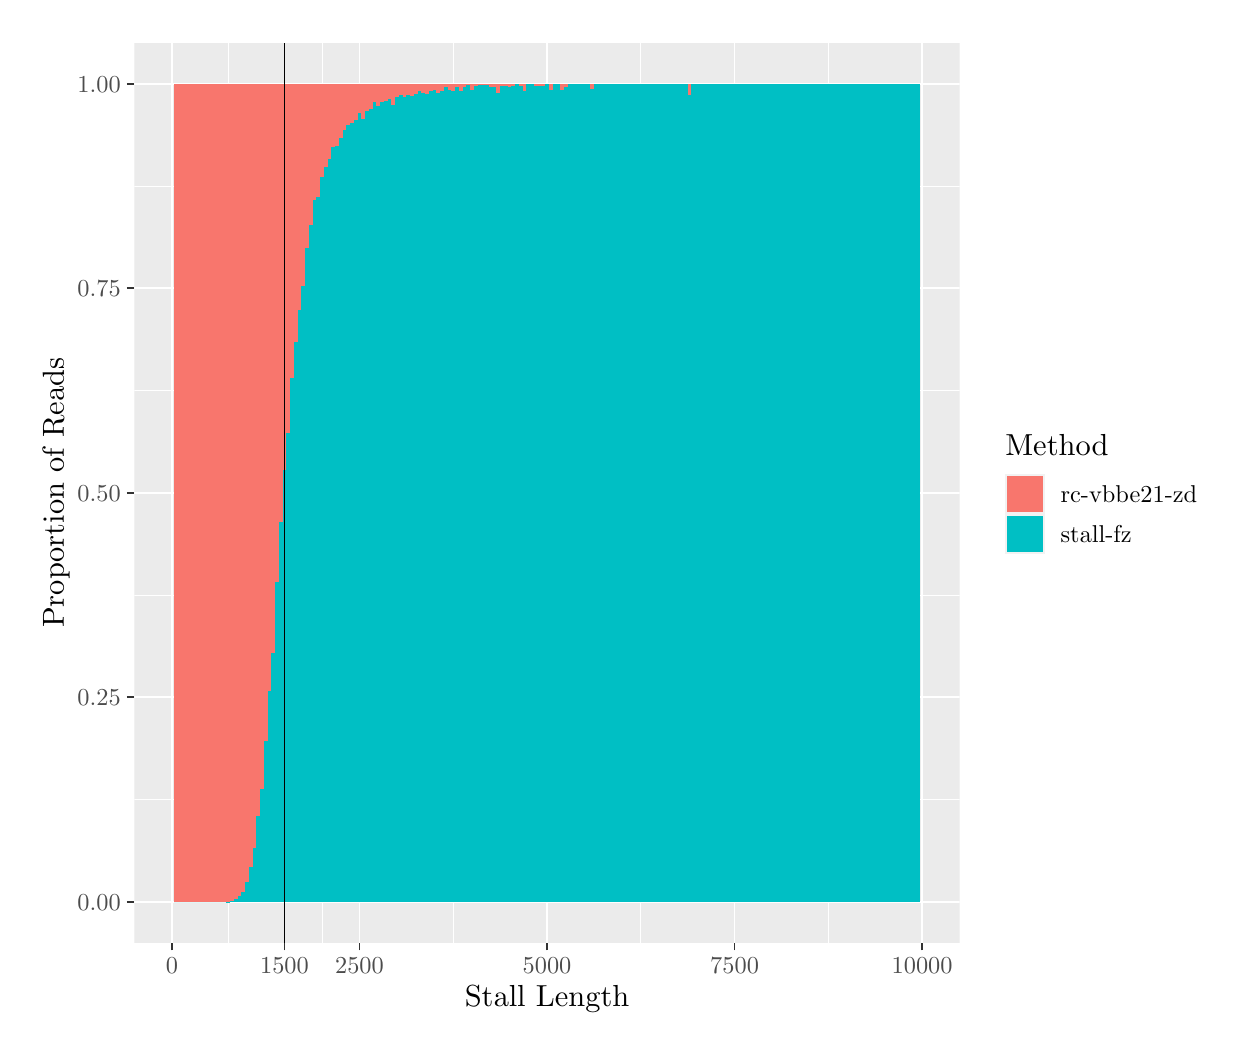
\begin{tikzpicture}[x=1pt,y=1pt]
\definecolor{fillColor}{RGB}{255,255,255}
\path[use as bounding box,fill=fillColor,fill opacity=0.00] (0,0) rectangle (433.62,361.35);
\begin{scope}
\path[clip] (  0.00,  0.00) rectangle (433.62,361.35);
\definecolor{drawColor}{RGB}{255,255,255}
\definecolor{fillColor}{RGB}{255,255,255}

\path[draw=drawColor,line width= 0.6pt,line join=round,line cap=round,fill=fillColor] (  0.00,  0.00) rectangle (433.62,361.35);
\end{scope}
\begin{scope}
\path[clip] ( 38.56, 30.69) rectangle (336.78,355.85);
\definecolor{fillColor}{gray}{0.92}

\path[fill=fillColor] ( 38.56, 30.69) rectangle (336.78,355.85);
\definecolor{drawColor}{RGB}{255,255,255}

\path[draw=drawColor,line width= 0.3pt,line join=round] ( 38.56, 82.42) --
	(336.78, 82.42);

\path[draw=drawColor,line width= 0.3pt,line join=round] ( 38.56,156.32) --
	(336.78,156.32);

\path[draw=drawColor,line width= 0.3pt,line join=round] ( 38.56,230.22) --
	(336.78,230.22);

\path[draw=drawColor,line width= 0.3pt,line join=round] ( 38.56,304.12) --
	(336.78,304.12);

\path[draw=drawColor,line width= 0.3pt,line join=round] ( 72.44, 30.69) --
	( 72.44,355.85);

\path[draw=drawColor,line width= 0.3pt,line join=round] (106.33, 30.69) --
	(106.33,355.85);

\path[draw=drawColor,line width= 0.3pt,line join=round] (153.78, 30.69) --
	(153.78,355.85);

\path[draw=drawColor,line width= 0.3pt,line join=round] (221.55, 30.69) --
	(221.55,355.85);

\path[draw=drawColor,line width= 0.3pt,line join=round] (289.33, 30.69) --
	(289.33,355.85);

\path[draw=drawColor,line width= 0.6pt,line join=round] ( 38.56, 45.47) --
	(336.78, 45.47);

\path[draw=drawColor,line width= 0.6pt,line join=round] ( 38.56,119.37) --
	(336.78,119.37);

\path[draw=drawColor,line width= 0.6pt,line join=round] ( 38.56,193.27) --
	(336.78,193.27);

\path[draw=drawColor,line width= 0.6pt,line join=round] ( 38.56,267.17) --
	(336.78,267.17);

\path[draw=drawColor,line width= 0.6pt,line join=round] ( 38.56,341.07) --
	(336.78,341.07);

\path[draw=drawColor,line width= 0.6pt,line join=round] ( 52.11, 30.69) --
	( 52.11,355.85);

\path[draw=drawColor,line width= 0.6pt,line join=round] ( 92.78, 30.69) --
	( 92.78,355.85);

\path[draw=drawColor,line width= 0.6pt,line join=round] (119.89, 30.69) --
	(119.89,355.85);

\path[draw=drawColor,line width= 0.6pt,line join=round] (187.67, 30.69) --
	(187.67,355.85);

\path[draw=drawColor,line width= 0.6pt,line join=round] (255.44, 30.69) --
	(255.44,355.85);

\path[draw=drawColor,line width= 0.6pt,line join=round] (323.22, 30.69) --
	(323.22,355.85);
\definecolor{fillColor}{RGB}{248,118,109}

\path[fill=fillColor] ( 52.79, 45.47) rectangle ( 54.14,341.07);

\path[fill=fillColor] ( 54.14, 45.47) rectangle ( 55.50,341.07);

\path[fill=fillColor] ( 55.50, 45.47) rectangle ( 56.85,341.07);

\path[fill=fillColor] ( 56.85, 45.47) rectangle ( 58.21,341.07);

\path[fill=fillColor] ( 58.21, 45.47) rectangle ( 59.57,341.07);

\path[fill=fillColor] ( 59.57, 45.47) rectangle ( 60.92,341.07);

\path[fill=fillColor] ( 60.92, 45.47) rectangle ( 62.28,341.07);

\path[fill=fillColor] ( 62.28, 45.47) rectangle ( 63.63,341.07);

\path[fill=fillColor] ( 63.63, 45.47) rectangle ( 64.99,341.07);

\path[fill=fillColor] ( 64.99, 45.47) rectangle ( 66.34,341.07);

\path[fill=fillColor] ( 66.34, 45.47) rectangle ( 67.70,341.07);

\path[fill=fillColor] ( 67.70, 45.47) rectangle ( 69.05,341.07);

\path[fill=fillColor] ( 69.05, 45.47) rectangle ( 70.41,341.07);

\path[fill=fillColor] ( 70.41, 45.47) rectangle ( 71.77,341.07);

\path[fill=fillColor] ( 71.77, 45.49) rectangle ( 73.12,341.07);

\path[fill=fillColor] ( 73.12, 45.92) rectangle ( 74.48,341.07);

\path[fill=fillColor] ( 74.48, 46.32) rectangle ( 75.83,341.07);

\path[fill=fillColor] ( 75.83, 47.48) rectangle ( 77.19,341.07);

\path[fill=fillColor] ( 77.19, 48.95) rectangle ( 78.54,341.07);

\path[fill=fillColor] ( 78.54, 52.57) rectangle ( 79.90,341.07);

\path[fill=fillColor] ( 79.90, 57.99) rectangle ( 81.25,341.07);

\path[fill=fillColor] ( 81.25, 64.89) rectangle ( 82.61,341.07);

\path[fill=fillColor] ( 82.61, 76.64) rectangle ( 83.97,341.07);

\path[fill=fillColor] ( 83.97, 86.37) rectangle ( 85.32,341.07);

\path[fill=fillColor] ( 85.32,103.73) rectangle ( 86.68,341.07);

\path[fill=fillColor] ( 86.68,121.80) rectangle ( 88.03,341.07);

\path[fill=fillColor] ( 88.03,135.40) rectangle ( 89.39,341.07);

\path[fill=fillColor] ( 89.39,161.09) rectangle ( 90.74,341.07);

\path[fill=fillColor] ( 90.74,182.61) rectangle ( 92.10,341.07);

\path[fill=fillColor] ( 92.10,201.69) rectangle ( 93.45,341.07);

\path[fill=fillColor] ( 93.45,214.83) rectangle ( 94.81,341.07);

\path[fill=fillColor] ( 94.81,234.71) rectangle ( 96.17,341.07);

\path[fill=fillColor] ( 96.17,247.88) rectangle ( 97.52,341.07);

\path[fill=fillColor] ( 97.52,259.33) rectangle ( 98.88,341.07);

\path[fill=fillColor] ( 98.88,268.04) rectangle (100.23,341.07);

\path[fill=fillColor] (100.23,281.77) rectangle (101.59,341.07);

\path[fill=fillColor] (101.59,290.15) rectangle (102.94,341.07);

\path[fill=fillColor] (102.94,299.08) rectangle (104.30,341.07);

\path[fill=fillColor] (104.30,300.06) rectangle (105.65,341.07);

\path[fill=fillColor] (105.65,307.56) rectangle (107.01,341.07);

\path[fill=fillColor] (107.01,310.83) rectangle (108.37,341.07);

\path[fill=fillColor] (108.37,313.71) rectangle (109.72,341.07);

\path[fill=fillColor] (109.72,318.32) rectangle (111.08,341.07);

\path[fill=fillColor] (111.08,318.61) rectangle (112.43,341.07);

\path[fill=fillColor] (112.43,321.62) rectangle (113.79,341.07);

\path[fill=fillColor] (113.79,324.46) rectangle (115.14,341.07);

\path[fill=fillColor] (115.14,326.00) rectangle (116.50,341.07);

\path[fill=fillColor] (116.50,326.99) rectangle (117.85,341.07);

\path[fill=fillColor] (117.85,328.11) rectangle (119.21,341.07);

\path[fill=fillColor] (119.21,330.49) rectangle (120.57,341.07);

\path[fill=fillColor] (120.57,328.48) rectangle (121.92,341.07);

\path[fill=fillColor] (121.92,331.26) rectangle (123.28,341.07);

\path[fill=fillColor] (123.28,331.80) rectangle (124.63,341.07);

\path[fill=fillColor] (124.63,334.52) rectangle (125.99,341.07);

\path[fill=fillColor] (125.99,333.20) rectangle (127.34,341.07);

\path[fill=fillColor] (127.34,334.33) rectangle (128.70,341.07);

\path[fill=fillColor] (128.70,334.88) rectangle (130.05,341.07);

\path[fill=fillColor] (130.05,335.69) rectangle (131.41,341.07);

\path[fill=fillColor] (131.41,333.30) rectangle (132.77,341.07);

\path[fill=fillColor] (132.77,336.15) rectangle (134.12,341.07);

\path[fill=fillColor] (134.12,336.96) rectangle (135.48,341.07);

\path[fill=fillColor] (135.48,336.47) rectangle (136.83,341.07);

\path[fill=fillColor] (136.83,337.17) rectangle (138.19,341.07);

\path[fill=fillColor] (138.19,336.65) rectangle (139.54,341.07);

\path[fill=fillColor] (139.54,337.46) rectangle (140.90,341.07);

\path[fill=fillColor] (140.90,338.46) rectangle (142.25,341.07);

\path[fill=fillColor] (142.25,337.85) rectangle (143.61,341.07);

\path[fill=fillColor] (143.61,337.32) rectangle (144.97,341.07);

\path[fill=fillColor] (144.97,338.55) rectangle (146.32,341.07);

\path[fill=fillColor] (146.32,338.66) rectangle (147.68,341.07);

\path[fill=fillColor] (147.68,337.90) rectangle (149.03,341.07);

\path[fill=fillColor] (149.03,338.44) rectangle (150.39,341.07);

\path[fill=fillColor] (150.39,339.75) rectangle (151.74,341.07);

\path[fill=fillColor] (151.74,338.93) rectangle (153.10,341.07);

\path[fill=fillColor] (153.10,338.63) rectangle (154.45,341.07);

\path[fill=fillColor] (154.45,339.91) rectangle (155.81,341.07);

\path[fill=fillColor] (155.81,338.52) rectangle (157.17,341.07);

\path[fill=fillColor] (157.17,339.80) rectangle (158.52,341.07);

\path[fill=fillColor] (158.52,340.63) rectangle (159.88,341.07);

\path[fill=fillColor] (159.88,338.85) rectangle (161.23,341.07);

\path[fill=fillColor] (161.23,340.14) rectangle (162.59,341.07);

\path[fill=fillColor] (162.59,340.59) rectangle (163.94,341.07);

\path[fill=fillColor] (163.94,340.58) rectangle (165.30,341.07);

\path[fill=fillColor] (165.30,340.53) rectangle (166.65,341.07);

\path[fill=fillColor] (166.65,339.91) rectangle (168.01,341.07);

\path[fill=fillColor] (168.01,339.95) rectangle (169.37,341.07);

\path[fill=fillColor] (169.37,337.56) rectangle (170.72,341.07);

\path[fill=fillColor] (170.72,340.42) rectangle (172.08,341.07);

\path[fill=fillColor] (172.08,340.40) rectangle (173.43,341.07);

\path[fill=fillColor] (173.43,339.76) rectangle (174.79,341.07);

\path[fill=fillColor] (174.79,340.31) rectangle (176.14,341.07);

\path[fill=fillColor] (176.14,341.07) rectangle (177.50,341.07);

\path[fill=fillColor] (177.50,340.29) rectangle (178.85,341.07);

\path[fill=fillColor] (178.85,338.62) rectangle (180.21,341.07);

\path[fill=fillColor] (180.21,341.07) rectangle (181.57,341.07);

\path[fill=fillColor] (181.57,341.07) rectangle (182.92,341.07);

\path[fill=fillColor] (182.92,340.22) rectangle (184.28,341.07);

\path[fill=fillColor] (184.28,340.23) rectangle (185.63,341.07);

\path[fill=fillColor] (185.63,340.17) rectangle (186.99,341.07);

\path[fill=fillColor] (186.99,341.07) rectangle (188.34,341.07);

\path[fill=fillColor] (188.34,338.90) rectangle (189.70,341.07);

\path[fill=fillColor] (189.70,341.07) rectangle (191.05,341.07);

\path[fill=fillColor] (191.05,341.07) rectangle (192.41,341.07);

\path[fill=fillColor] (192.41,338.74) rectangle (193.77,341.07);

\path[fill=fillColor] (193.77,339.77) rectangle (195.12,341.07);

\path[fill=fillColor] (195.12,341.07) rectangle (196.48,341.07);

\path[fill=fillColor] (196.48,341.07) rectangle (197.83,341.07);

\path[fill=fillColor] (197.83,341.07) rectangle (199.19,341.07);

\path[fill=fillColor] (199.19,341.07) rectangle (200.54,341.07);

\path[fill=fillColor] (200.54,341.07) rectangle (201.90,341.07);

\path[fill=fillColor] (201.90,341.07) rectangle (203.25,341.07);

\path[fill=fillColor] (203.25,339.32) rectangle (204.61,341.07);

\path[fill=fillColor] (204.61,341.07) rectangle (205.97,341.07);

\path[fill=fillColor] (205.97,341.07) rectangle (207.32,341.07);

\path[fill=fillColor] (207.32,341.07) rectangle (208.68,341.07);

\path[fill=fillColor] (208.68,341.07) rectangle (210.03,341.07);

\path[fill=fillColor] (210.03,341.07) rectangle (211.39,341.07);

\path[fill=fillColor] (211.39,341.07) rectangle (212.74,341.07);

\path[fill=fillColor] (212.74,341.07) rectangle (214.10,341.07);

\path[fill=fillColor] (214.10,341.07) rectangle (215.45,341.07);

\path[fill=fillColor] (215.45,341.07) rectangle (216.81,341.07);

\path[fill=fillColor] (216.81,341.07) rectangle (218.17,341.07);

\path[fill=fillColor] (218.17,341.07) rectangle (219.52,341.07);

\path[fill=fillColor] (219.52,341.07) rectangle (220.88,341.07);

\path[fill=fillColor] (220.88,341.07) rectangle (222.23,341.07);

\path[fill=fillColor] (222.23,341.07) rectangle (223.59,341.07);

\path[fill=fillColor] (223.59,341.07) rectangle (224.94,341.07);

\path[fill=fillColor] (224.94,341.07) rectangle (226.30,341.07);

\path[fill=fillColor] (226.30,341.07) rectangle (227.65,341.07);

\path[fill=fillColor] (227.65,341.07) rectangle (229.01,341.07);

\path[fill=fillColor] (229.01,341.07) rectangle (230.37,341.07);

\path[fill=fillColor] (230.37,341.07) rectangle (231.72,341.07);

\path[fill=fillColor] (231.72,341.07) rectangle (233.08,341.07);

\path[fill=fillColor] (233.08,341.07) rectangle (234.43,341.07);

\path[fill=fillColor] (234.43,341.07) rectangle (235.79,341.07);

\path[fill=fillColor] (235.79,341.07) rectangle (237.14,341.07);

\path[fill=fillColor] (237.14,341.07) rectangle (238.50,341.07);

\path[fill=fillColor] (238.50,337.13) rectangle (239.85,341.07);

\path[fill=fillColor] (239.85,341.07) rectangle (241.21,341.07);

\path[fill=fillColor] (241.21,341.07) rectangle (242.56,341.07);

\path[fill=fillColor] (242.56,341.07) rectangle (243.92,341.07);

\path[fill=fillColor] (243.92,341.07) rectangle (245.28,341.07);

\path[fill=fillColor] (245.28,341.07) rectangle (246.63,341.07);

\path[fill=fillColor] (246.63,341.07) rectangle (247.99,341.07);

\path[fill=fillColor] (247.99,341.07) rectangle (249.34,341.07);

\path[fill=fillColor] (249.34,341.07) rectangle (250.70,341.07);

\path[fill=fillColor] (250.70,341.07) rectangle (252.05,341.07);

\path[fill=fillColor] (252.05,341.07) rectangle (253.41,341.07);

\path[fill=fillColor] (253.41,341.07) rectangle (254.76,341.07);

\path[fill=fillColor] (254.76,341.07) rectangle (256.12,341.07);

\path[fill=fillColor] (256.12,341.07) rectangle (257.48,341.07);

\path[fill=fillColor] (257.48,341.07) rectangle (258.83,341.07);

\path[fill=fillColor] (258.83,341.07) rectangle (260.19,341.07);

\path[fill=fillColor] (260.19,341.07) rectangle (261.54,341.07);

\path[fill=fillColor] (261.54,341.07) rectangle (262.90,341.07);

\path[fill=fillColor] (262.90,341.07) rectangle (264.25,341.07);

\path[fill=fillColor] (264.25,341.07) rectangle (265.61,341.07);

\path[fill=fillColor] (265.61,341.07) rectangle (266.96,341.07);

\path[fill=fillColor] (266.96,341.07) rectangle (268.32,341.07);

\path[fill=fillColor] (268.32,341.07) rectangle (269.68,341.07);

\path[fill=fillColor] (269.68,341.07) rectangle (271.03,341.07);

\path[fill=fillColor] (271.03,341.07) rectangle (272.39,341.07);

\path[fill=fillColor] (272.39,341.07) rectangle (273.74,341.07);

\path[fill=fillColor] (273.74,341.07) rectangle (275.10,341.07);

\path[fill=fillColor] (275.10,341.07) rectangle (276.45,341.07);

\path[fill=fillColor] (276.45,341.07) rectangle (277.81,341.07);

\path[fill=fillColor] (277.81,341.07) rectangle (279.16,341.07);

\path[fill=fillColor] (279.16,341.07) rectangle (280.52,341.07);

\path[fill=fillColor] (280.52,341.07) rectangle (281.88,341.07);

\path[fill=fillColor] (281.88,341.07) rectangle (283.23,341.07);

\path[fill=fillColor] (283.23,341.07) rectangle (284.59,341.07);

\path[fill=fillColor] (284.59,341.07) rectangle (285.94,341.07);

\path[fill=fillColor] (285.94,341.07) rectangle (287.30,341.07);

\path[fill=fillColor] (287.30,341.07) rectangle (288.65,341.07);

\path[fill=fillColor] (288.65,341.07) rectangle (290.01,341.07);

\path[fill=fillColor] (290.01,341.07) rectangle (291.36,341.07);

\path[fill=fillColor] (291.36,341.07) rectangle (292.72,341.07);

\path[fill=fillColor] (292.72,341.07) rectangle (294.08,341.07);

\path[fill=fillColor] (294.08,341.07) rectangle (295.43,341.07);

\path[fill=fillColor] (295.43,341.07) rectangle (296.79,341.07);

\path[fill=fillColor] (296.79,341.07) rectangle (298.14,341.07);

\path[fill=fillColor] (298.14,341.07) rectangle (299.50,341.07);

\path[fill=fillColor] (299.50,341.07) rectangle (300.85,341.07);

\path[fill=fillColor] (300.85,341.07) rectangle (302.21,341.07);

\path[fill=fillColor] (302.21,341.07) rectangle (303.56,341.07);

\path[fill=fillColor] (303.56,341.07) rectangle (304.92,341.07);

\path[fill=fillColor] (304.92,341.07) rectangle (306.28,341.07);

\path[fill=fillColor] (306.28,341.07) rectangle (307.63,341.07);

\path[fill=fillColor] (307.63,341.07) rectangle (308.99,341.07);

\path[fill=fillColor] (308.99,341.07) rectangle (310.34,341.07);

\path[fill=fillColor] (310.34,341.07) rectangle (311.70,341.07);

\path[fill=fillColor] (311.70,341.07) rectangle (313.05,341.07);

\path[fill=fillColor] (313.05,341.07) rectangle (314.41,341.07);

\path[fill=fillColor] (314.41,341.07) rectangle (315.76,341.07);

\path[fill=fillColor] (315.76,341.07) rectangle (317.12,341.07);

\path[fill=fillColor] (317.12,341.07) rectangle (318.48,341.07);

\path[fill=fillColor] (318.48,341.07) rectangle (319.83,341.07);

\path[fill=fillColor] (319.83,341.07) rectangle (321.19,341.07);

\path[fill=fillColor] (321.19,341.07) rectangle (322.54,341.07);
\definecolor{fillColor}{RGB}{0,191,196}

\path[fill=fillColor] ( 52.79, 45.47) rectangle ( 54.14, 45.47);

\path[fill=fillColor] ( 54.14, 45.47) rectangle ( 55.50, 45.47);

\path[fill=fillColor] ( 55.50, 45.47) rectangle ( 56.85, 45.47);

\path[fill=fillColor] ( 56.85, 45.47) rectangle ( 58.21, 45.47);

\path[fill=fillColor] ( 58.21, 45.47) rectangle ( 59.57, 45.47);

\path[fill=fillColor] ( 59.57, 45.47) rectangle ( 60.92, 45.47);

\path[fill=fillColor] ( 60.92, 45.47) rectangle ( 62.28, 45.47);

\path[fill=fillColor] ( 62.28, 45.47) rectangle ( 63.63, 45.47);

\path[fill=fillColor] ( 63.63, 45.47) rectangle ( 64.99, 45.47);

\path[fill=fillColor] ( 64.99, 45.47) rectangle ( 66.34, 45.47);

\path[fill=fillColor] ( 66.34, 45.47) rectangle ( 67.70, 45.47);

\path[fill=fillColor] ( 67.70, 45.47) rectangle ( 69.05, 45.47);

\path[fill=fillColor] ( 69.05, 45.47) rectangle ( 70.41, 45.47);

\path[fill=fillColor] ( 70.41, 45.47) rectangle ( 71.77, 45.47);

\path[fill=fillColor] ( 71.77, 45.47) rectangle ( 73.12, 45.49);

\path[fill=fillColor] ( 73.12, 45.47) rectangle ( 74.48, 45.92);

\path[fill=fillColor] ( 74.48, 45.47) rectangle ( 75.83, 46.32);

\path[fill=fillColor] ( 75.83, 45.47) rectangle ( 77.19, 47.48);

\path[fill=fillColor] ( 77.19, 45.47) rectangle ( 78.54, 48.95);

\path[fill=fillColor] ( 78.54, 45.47) rectangle ( 79.90, 52.57);

\path[fill=fillColor] ( 79.90, 45.47) rectangle ( 81.25, 57.99);

\path[fill=fillColor] ( 81.25, 45.47) rectangle ( 82.61, 64.89);

\path[fill=fillColor] ( 82.61, 45.47) rectangle ( 83.97, 76.64);

\path[fill=fillColor] ( 83.97, 45.47) rectangle ( 85.32, 86.37);

\path[fill=fillColor] ( 85.32, 45.47) rectangle ( 86.68,103.73);

\path[fill=fillColor] ( 86.68, 45.47) rectangle ( 88.03,121.80);

\path[fill=fillColor] ( 88.03, 45.47) rectangle ( 89.39,135.40);

\path[fill=fillColor] ( 89.39, 45.47) rectangle ( 90.74,161.09);

\path[fill=fillColor] ( 90.74, 45.47) rectangle ( 92.10,182.61);

\path[fill=fillColor] ( 92.10, 45.47) rectangle ( 93.45,201.69);

\path[fill=fillColor] ( 93.45, 45.47) rectangle ( 94.81,214.83);

\path[fill=fillColor] ( 94.81, 45.47) rectangle ( 96.17,234.71);

\path[fill=fillColor] ( 96.17, 45.47) rectangle ( 97.52,247.88);

\path[fill=fillColor] ( 97.52, 45.47) rectangle ( 98.88,259.33);

\path[fill=fillColor] ( 98.88, 45.47) rectangle (100.23,268.04);

\path[fill=fillColor] (100.23, 45.47) rectangle (101.59,281.77);

\path[fill=fillColor] (101.59, 45.47) rectangle (102.94,290.15);

\path[fill=fillColor] (102.94, 45.47) rectangle (104.30,299.08);

\path[fill=fillColor] (104.30, 45.47) rectangle (105.65,300.06);

\path[fill=fillColor] (105.65, 45.47) rectangle (107.01,307.56);

\path[fill=fillColor] (107.01, 45.47) rectangle (108.37,310.83);

\path[fill=fillColor] (108.37, 45.47) rectangle (109.72,313.71);

\path[fill=fillColor] (109.72, 45.47) rectangle (111.08,318.32);

\path[fill=fillColor] (111.08, 45.47) rectangle (112.43,318.61);

\path[fill=fillColor] (112.43, 45.47) rectangle (113.79,321.62);

\path[fill=fillColor] (113.79, 45.47) rectangle (115.14,324.46);

\path[fill=fillColor] (115.14, 45.47) rectangle (116.50,326.00);

\path[fill=fillColor] (116.50, 45.47) rectangle (117.85,326.99);

\path[fill=fillColor] (117.85, 45.47) rectangle (119.21,328.11);

\path[fill=fillColor] (119.21, 45.47) rectangle (120.57,330.49);

\path[fill=fillColor] (120.57, 45.47) rectangle (121.92,328.48);

\path[fill=fillColor] (121.92, 45.47) rectangle (123.28,331.26);

\path[fill=fillColor] (123.28, 45.47) rectangle (124.63,331.80);

\path[fill=fillColor] (124.63, 45.47) rectangle (125.99,334.52);

\path[fill=fillColor] (125.99, 45.47) rectangle (127.34,333.20);

\path[fill=fillColor] (127.34, 45.47) rectangle (128.70,334.33);

\path[fill=fillColor] (128.70, 45.47) rectangle (130.05,334.88);

\path[fill=fillColor] (130.05, 45.47) rectangle (131.41,335.69);

\path[fill=fillColor] (131.41, 45.47) rectangle (132.77,333.30);

\path[fill=fillColor] (132.77, 45.47) rectangle (134.12,336.15);

\path[fill=fillColor] (134.12, 45.47) rectangle (135.48,336.96);

\path[fill=fillColor] (135.48, 45.47) rectangle (136.83,336.47);

\path[fill=fillColor] (136.83, 45.47) rectangle (138.19,337.17);

\path[fill=fillColor] (138.19, 45.47) rectangle (139.54,336.65);

\path[fill=fillColor] (139.54, 45.47) rectangle (140.90,337.46);

\path[fill=fillColor] (140.90, 45.47) rectangle (142.25,338.46);

\path[fill=fillColor] (142.25, 45.47) rectangle (143.61,337.85);

\path[fill=fillColor] (143.61, 45.47) rectangle (144.97,337.32);

\path[fill=fillColor] (144.97, 45.47) rectangle (146.32,338.55);

\path[fill=fillColor] (146.32, 45.47) rectangle (147.68,338.66);

\path[fill=fillColor] (147.68, 45.47) rectangle (149.03,337.90);

\path[fill=fillColor] (149.03, 45.47) rectangle (150.39,338.44);

\path[fill=fillColor] (150.39, 45.47) rectangle (151.74,339.75);

\path[fill=fillColor] (151.74, 45.47) rectangle (153.10,338.93);

\path[fill=fillColor] (153.10, 45.47) rectangle (154.45,338.63);

\path[fill=fillColor] (154.45, 45.47) rectangle (155.81,339.91);

\path[fill=fillColor] (155.81, 45.47) rectangle (157.17,338.52);

\path[fill=fillColor] (157.17, 45.47) rectangle (158.52,339.80);

\path[fill=fillColor] (158.52, 45.47) rectangle (159.88,340.63);

\path[fill=fillColor] (159.88, 45.47) rectangle (161.23,338.85);

\path[fill=fillColor] (161.23, 45.47) rectangle (162.59,340.14);

\path[fill=fillColor] (162.59, 45.47) rectangle (163.94,340.59);

\path[fill=fillColor] (163.94, 45.47) rectangle (165.30,340.58);

\path[fill=fillColor] (165.30, 45.47) rectangle (166.65,340.53);

\path[fill=fillColor] (166.65, 45.47) rectangle (168.01,339.91);

\path[fill=fillColor] (168.01, 45.47) rectangle (169.37,339.95);

\path[fill=fillColor] (169.37, 45.47) rectangle (170.72,337.56);

\path[fill=fillColor] (170.72, 45.47) rectangle (172.08,340.42);

\path[fill=fillColor] (172.08, 45.47) rectangle (173.43,340.40);

\path[fill=fillColor] (173.43, 45.47) rectangle (174.79,339.76);

\path[fill=fillColor] (174.79, 45.47) rectangle (176.14,340.31);

\path[fill=fillColor] (176.14, 45.47) rectangle (177.50,341.07);

\path[fill=fillColor] (177.50, 45.47) rectangle (178.85,340.29);

\path[fill=fillColor] (178.85, 45.47) rectangle (180.21,338.62);

\path[fill=fillColor] (180.21, 45.47) rectangle (181.57,341.07);

\path[fill=fillColor] (181.57, 45.47) rectangle (182.92,341.07);

\path[fill=fillColor] (182.92, 45.47) rectangle (184.28,340.22);

\path[fill=fillColor] (184.28, 45.47) rectangle (185.63,340.23);

\path[fill=fillColor] (185.63, 45.47) rectangle (186.99,340.17);

\path[fill=fillColor] (186.99, 45.47) rectangle (188.34,341.07);

\path[fill=fillColor] (188.34, 45.47) rectangle (189.70,338.90);

\path[fill=fillColor] (189.70, 45.47) rectangle (191.05,341.07);

\path[fill=fillColor] (191.05, 45.47) rectangle (192.41,341.07);

\path[fill=fillColor] (192.41, 45.47) rectangle (193.77,338.74);

\path[fill=fillColor] (193.77, 45.47) rectangle (195.12,339.77);

\path[fill=fillColor] (195.12, 45.47) rectangle (196.48,341.07);

\path[fill=fillColor] (196.48, 45.47) rectangle (197.83,341.07);

\path[fill=fillColor] (197.83, 45.47) rectangle (199.19,341.07);

\path[fill=fillColor] (199.19, 45.47) rectangle (200.54,341.07);

\path[fill=fillColor] (200.54, 45.47) rectangle (201.90,341.07);

\path[fill=fillColor] (201.90, 45.47) rectangle (203.25,341.07);

\path[fill=fillColor] (203.25, 45.47) rectangle (204.61,339.32);

\path[fill=fillColor] (204.61, 45.47) rectangle (205.97,341.07);

\path[fill=fillColor] (205.97, 45.47) rectangle (207.32,341.07);

\path[fill=fillColor] (207.32, 45.47) rectangle (208.68,341.07);

\path[fill=fillColor] (208.68, 45.47) rectangle (210.03,341.07);

\path[fill=fillColor] (210.03, 45.47) rectangle (211.39,341.07);

\path[fill=fillColor] (211.39, 45.47) rectangle (212.74,341.07);

\path[fill=fillColor] (212.74, 45.47) rectangle (214.10,341.07);

\path[fill=fillColor] (214.10, 45.47) rectangle (215.45,341.07);

\path[fill=fillColor] (215.45, 45.47) rectangle (216.81,341.07);

\path[fill=fillColor] (216.81, 45.47) rectangle (218.17,341.07);

\path[fill=fillColor] (218.17, 45.47) rectangle (219.52,341.07);

\path[fill=fillColor] (219.52, 45.47) rectangle (220.88,341.07);

\path[fill=fillColor] (220.88, 45.47) rectangle (222.23,341.07);

\path[fill=fillColor] (222.23, 45.47) rectangle (223.59,341.07);

\path[fill=fillColor] (223.59, 45.47) rectangle (224.94,341.07);

\path[fill=fillColor] (224.94, 45.47) rectangle (226.30,341.07);

\path[fill=fillColor] (226.30, 45.47) rectangle (227.65,341.07);

\path[fill=fillColor] (227.65, 45.47) rectangle (229.01,341.07);

\path[fill=fillColor] (229.01, 45.47) rectangle (230.37,341.07);

\path[fill=fillColor] (230.37, 45.47) rectangle (231.72,341.07);

\path[fill=fillColor] (231.72, 45.47) rectangle (233.08,341.07);

\path[fill=fillColor] (233.08, 45.47) rectangle (234.43,341.07);

\path[fill=fillColor] (234.43, 45.47) rectangle (235.79,341.07);

\path[fill=fillColor] (235.79, 45.47) rectangle (237.14,341.07);

\path[fill=fillColor] (237.14, 45.47) rectangle (238.50,341.07);

\path[fill=fillColor] (238.50, 45.47) rectangle (239.85,337.13);

\path[fill=fillColor] (239.85, 45.47) rectangle (241.21,341.07);

\path[fill=fillColor] (241.21, 45.47) rectangle (242.56,341.07);

\path[fill=fillColor] (242.56, 45.47) rectangle (243.92,341.07);

\path[fill=fillColor] (243.92, 45.47) rectangle (245.28,341.07);

\path[fill=fillColor] (245.28, 45.47) rectangle (246.63,341.07);

\path[fill=fillColor] (246.63, 45.47) rectangle (247.99,341.07);

\path[fill=fillColor] (247.99, 45.47) rectangle (249.34,341.07);

\path[fill=fillColor] (249.34, 45.47) rectangle (250.70,341.07);

\path[fill=fillColor] (250.70, 45.47) rectangle (252.05,341.07);

\path[fill=fillColor] (252.05, 45.47) rectangle (253.41,341.07);

\path[fill=fillColor] (253.41, 45.47) rectangle (254.76,341.07);

\path[fill=fillColor] (254.76, 45.47) rectangle (256.12,341.07);

\path[fill=fillColor] (256.12, 45.47) rectangle (257.48,341.07);

\path[fill=fillColor] (257.48, 45.47) rectangle (258.83,341.07);

\path[fill=fillColor] (258.83, 45.47) rectangle (260.19,341.07);

\path[fill=fillColor] (260.19, 45.47) rectangle (261.54,341.07);

\path[fill=fillColor] (261.54, 45.47) rectangle (262.90,341.07);

\path[fill=fillColor] (262.90, 45.47) rectangle (264.25,341.07);

\path[fill=fillColor] (264.25, 45.47) rectangle (265.61,341.07);

\path[fill=fillColor] (265.61, 45.47) rectangle (266.96,341.07);

\path[fill=fillColor] (266.96, 45.47) rectangle (268.32,341.07);

\path[fill=fillColor] (268.32, 45.47) rectangle (269.68,341.07);

\path[fill=fillColor] (269.68, 45.47) rectangle (271.03,341.07);

\path[fill=fillColor] (271.03, 45.47) rectangle (272.39,341.07);

\path[fill=fillColor] (272.39, 45.47) rectangle (273.74,341.07);

\path[fill=fillColor] (273.74, 45.47) rectangle (275.10,341.07);

\path[fill=fillColor] (275.10, 45.47) rectangle (276.45,341.07);

\path[fill=fillColor] (276.45, 45.47) rectangle (277.81,341.07);

\path[fill=fillColor] (277.81, 45.47) rectangle (279.16,341.07);

\path[fill=fillColor] (279.16, 45.47) rectangle (280.52,341.07);

\path[fill=fillColor] (280.52, 45.47) rectangle (281.88,341.07);

\path[fill=fillColor] (281.88, 45.47) rectangle (283.23,341.07);

\path[fill=fillColor] (283.23, 45.47) rectangle (284.59,341.07);

\path[fill=fillColor] (284.59, 45.47) rectangle (285.94,341.07);

\path[fill=fillColor] (285.94, 45.47) rectangle (287.30,341.07);

\path[fill=fillColor] (287.30, 45.47) rectangle (288.65,341.07);

\path[fill=fillColor] (288.65, 45.47) rectangle (290.01,341.07);

\path[fill=fillColor] (290.01, 45.47) rectangle (291.36,341.07);

\path[fill=fillColor] (291.36, 45.47) rectangle (292.72,341.07);

\path[fill=fillColor] (292.72, 45.47) rectangle (294.08,341.07);

\path[fill=fillColor] (294.08, 45.47) rectangle (295.43,341.07);

\path[fill=fillColor] (295.43, 45.47) rectangle (296.79,341.07);

\path[fill=fillColor] (296.79, 45.47) rectangle (298.14,341.07);

\path[fill=fillColor] (298.14, 45.47) rectangle (299.50,341.07);

\path[fill=fillColor] (299.50, 45.47) rectangle (300.85,341.07);

\path[fill=fillColor] (300.85, 45.47) rectangle (302.21,341.07);

\path[fill=fillColor] (302.21, 45.47) rectangle (303.56,341.07);

\path[fill=fillColor] (303.56, 45.47) rectangle (304.92,341.07);

\path[fill=fillColor] (304.92, 45.47) rectangle (306.28,341.07);

\path[fill=fillColor] (306.28, 45.47) rectangle (307.63,341.07);

\path[fill=fillColor] (307.63, 45.47) rectangle (308.99,341.07);

\path[fill=fillColor] (308.99, 45.47) rectangle (310.34,341.07);

\path[fill=fillColor] (310.34, 45.47) rectangle (311.70,341.07);

\path[fill=fillColor] (311.70, 45.47) rectangle (313.05,341.07);

\path[fill=fillColor] (313.05, 45.47) rectangle (314.41,341.07);

\path[fill=fillColor] (314.41, 45.47) rectangle (315.76,341.07);

\path[fill=fillColor] (315.76, 45.47) rectangle (317.12,341.07);

\path[fill=fillColor] (317.12, 45.47) rectangle (318.48,341.07);

\path[fill=fillColor] (318.48, 45.47) rectangle (319.83,341.07);

\path[fill=fillColor] (319.83, 45.47) rectangle (321.19,341.07);

\path[fill=fillColor] (321.19, 45.47) rectangle (322.54,341.07);
\definecolor{drawColor}{RGB}{0,0,0}

\path[draw=drawColor,line width= 0.6pt,line join=round] ( 92.78, 30.69) -- ( 92.78,355.85);
\end{scope}
\begin{scope}
\path[clip] (  0.00,  0.00) rectangle (433.62,361.35);
\definecolor{drawColor}{gray}{0.30}

\node[text=drawColor,anchor=base east,inner sep=0pt, outer sep=0pt, scale=  0.88] at ( 33.61, 42.44) {0.00};

\node[text=drawColor,anchor=base east,inner sep=0pt, outer sep=0pt, scale=  0.88] at ( 33.61,116.34) {0.25};

\node[text=drawColor,anchor=base east,inner sep=0pt, outer sep=0pt, scale=  0.88] at ( 33.61,190.24) {0.50};

\node[text=drawColor,anchor=base east,inner sep=0pt, outer sep=0pt, scale=  0.88] at ( 33.61,264.14) {0.75};

\node[text=drawColor,anchor=base east,inner sep=0pt, outer sep=0pt, scale=  0.88] at ( 33.61,338.04) {1.00};
\end{scope}
\begin{scope}
\path[clip] (  0.00,  0.00) rectangle (433.62,361.35);
\definecolor{drawColor}{gray}{0.20}

\path[draw=drawColor,line width= 0.6pt,line join=round] ( 35.81, 45.47) --
	( 38.56, 45.47);

\path[draw=drawColor,line width= 0.6pt,line join=round] ( 35.81,119.37) --
	( 38.56,119.37);

\path[draw=drawColor,line width= 0.6pt,line join=round] ( 35.81,193.27) --
	( 38.56,193.27);

\path[draw=drawColor,line width= 0.6pt,line join=round] ( 35.81,267.17) --
	( 38.56,267.17);

\path[draw=drawColor,line width= 0.6pt,line join=round] ( 35.81,341.07) --
	( 38.56,341.07);
\end{scope}
\begin{scope}
\path[clip] (  0.00,  0.00) rectangle (433.62,361.35);
\definecolor{drawColor}{gray}{0.20}

\path[draw=drawColor,line width= 0.6pt,line join=round] ( 52.11, 27.94) --
	( 52.11, 30.69);

\path[draw=drawColor,line width= 0.6pt,line join=round] ( 92.78, 27.94) --
	( 92.78, 30.69);

\path[draw=drawColor,line width= 0.6pt,line join=round] (119.89, 27.94) --
	(119.89, 30.69);

\path[draw=drawColor,line width= 0.6pt,line join=round] (187.67, 27.94) --
	(187.67, 30.69);

\path[draw=drawColor,line width= 0.6pt,line join=round] (255.44, 27.94) --
	(255.44, 30.69);

\path[draw=drawColor,line width= 0.6pt,line join=round] (323.22, 27.94) --
	(323.22, 30.69);
\end{scope}
\begin{scope}
\path[clip] (  0.00,  0.00) rectangle (433.62,361.35);
\definecolor{drawColor}{gray}{0.30}

\node[text=drawColor,anchor=base,inner sep=0pt, outer sep=0pt, scale=  0.88] at ( 52.11, 19.68) {0};

\node[text=drawColor,anchor=base,inner sep=0pt, outer sep=0pt, scale=  0.88] at ( 92.78, 19.68) {1500};

\node[text=drawColor,anchor=base,inner sep=0pt, outer sep=0pt, scale=  0.88] at (119.89, 19.68) {2500};

\node[text=drawColor,anchor=base,inner sep=0pt, outer sep=0pt, scale=  0.88] at (187.67, 19.68) {5000};

\node[text=drawColor,anchor=base,inner sep=0pt, outer sep=0pt, scale=  0.88] at (255.44, 19.68) {7500};

\node[text=drawColor,anchor=base,inner sep=0pt, outer sep=0pt, scale=  0.88] at (323.22, 19.68) {10000};
\end{scope}
\begin{scope}
\path[clip] (  0.00,  0.00) rectangle (433.62,361.35);
\definecolor{drawColor}{RGB}{0,0,0}

\node[text=drawColor,anchor=base,inner sep=0pt, outer sep=0pt, scale=  1.10] at (187.67,  7.64) {Stall Length};
\end{scope}
\begin{scope}
\path[clip] (  0.00,  0.00) rectangle (433.62,361.35);
\definecolor{drawColor}{RGB}{0,0,0}

\node[text=drawColor,rotate= 90.00,anchor=base,inner sep=0pt, outer sep=0pt, scale=  1.10] at ( 13.08,193.27) {Proportion of Reads};
\end{scope}
\begin{scope}
\path[clip] (  0.00,  0.00) rectangle (433.62,361.35);
\definecolor{fillColor}{RGB}{255,255,255}

\path[fill=fillColor] (347.78,165.71) rectangle (428.12,220.83);
\end{scope}
\begin{scope}
\path[clip] (  0.00,  0.00) rectangle (433.62,361.35);
\definecolor{drawColor}{RGB}{0,0,0}

\node[text=drawColor,anchor=base west,inner sep=0pt, outer sep=0pt, scale=  1.10] at (353.28,206.68) {Method};
\end{scope}
\begin{scope}
\path[clip] (  0.00,  0.00) rectangle (433.62,361.35);
\definecolor{fillColor}{gray}{0.95}

\path[fill=fillColor] (353.28,185.66) rectangle (367.73,200.11);
\end{scope}
\begin{scope}
\path[clip] (  0.00,  0.00) rectangle (433.62,361.35);
\definecolor{fillColor}{RGB}{248,118,109}

\path[fill=fillColor] (353.99,186.37) rectangle (367.02,199.40);
\end{scope}
\begin{scope}
\path[clip] (  0.00,  0.00) rectangle (433.62,361.35);
\definecolor{fillColor}{gray}{0.95}

\path[fill=fillColor] (353.28,171.21) rectangle (367.73,185.66);
\end{scope}
\begin{scope}
\path[clip] (  0.00,  0.00) rectangle (433.62,361.35);
\definecolor{fillColor}{RGB}{0,191,196}

\path[fill=fillColor] (353.99,171.92) rectangle (367.02,184.95);
\end{scope}
\begin{scope}
\path[clip] (  0.00,  0.00) rectangle (433.62,361.35);
\definecolor{drawColor}{RGB}{0,0,0}

\node[text=drawColor,anchor=base west,inner sep=0pt, outer sep=0pt, scale=  0.88] at (373.23,189.86) {rc-vbbe21-zd};
\end{scope}
\begin{scope}
\path[clip] (  0.00,  0.00) rectangle (433.62,361.35);
\definecolor{drawColor}{RGB}{0,0,0}

\node[text=drawColor,anchor=base west,inner sep=0pt, outer sep=0pt, scale=  0.88] at (373.23,175.40) {stall-fz};
\end{scope}
\end{tikzpicture}

\caption{\label{fig:stall-ratio}The 100\% stacked histogram of the compression
	methods with the highest compression ratio for all the reads in the data
	versus their stall length. Reads with a stall length $\sim$1500 and
	greater are more likely to be compressed smaller using stall-fz than
	rc-vbbe21-zd.}
\end{figure}

\begin{figure}
\centering
%\input{plots/reads.blow5.test.svbbe21.read.best}
\includegraphics[scale=0.7]{plots/reads.blow5.test.svbbe21.read.update.best.pdf}
	\caption[A scatter plot of the compression methods with
the highest compression ratio on each read out of rc01s-vbbe21-zd and stall-fz.]{\label{fig:stall-best}A scatter plot of the compression methods with
the highest compression ratio on each read out of rc01s-vbbe21-zd and stall-fz. The
best compression ratio is plotted against the length of the read's stall. Reads
with a stall length $\sim$1500 and greater are more likely to be compressed
smaller with stall-fz rather than rc01s-vbbe21-zd.}
\end{figure}


\subsection{The DNA Section}

\begin{figure}
\centering
% Created by tikzDevice version 0.12.3.1 on 2022-10-19 12:01:19
% !TEX encoding = UTF-8 Unicode
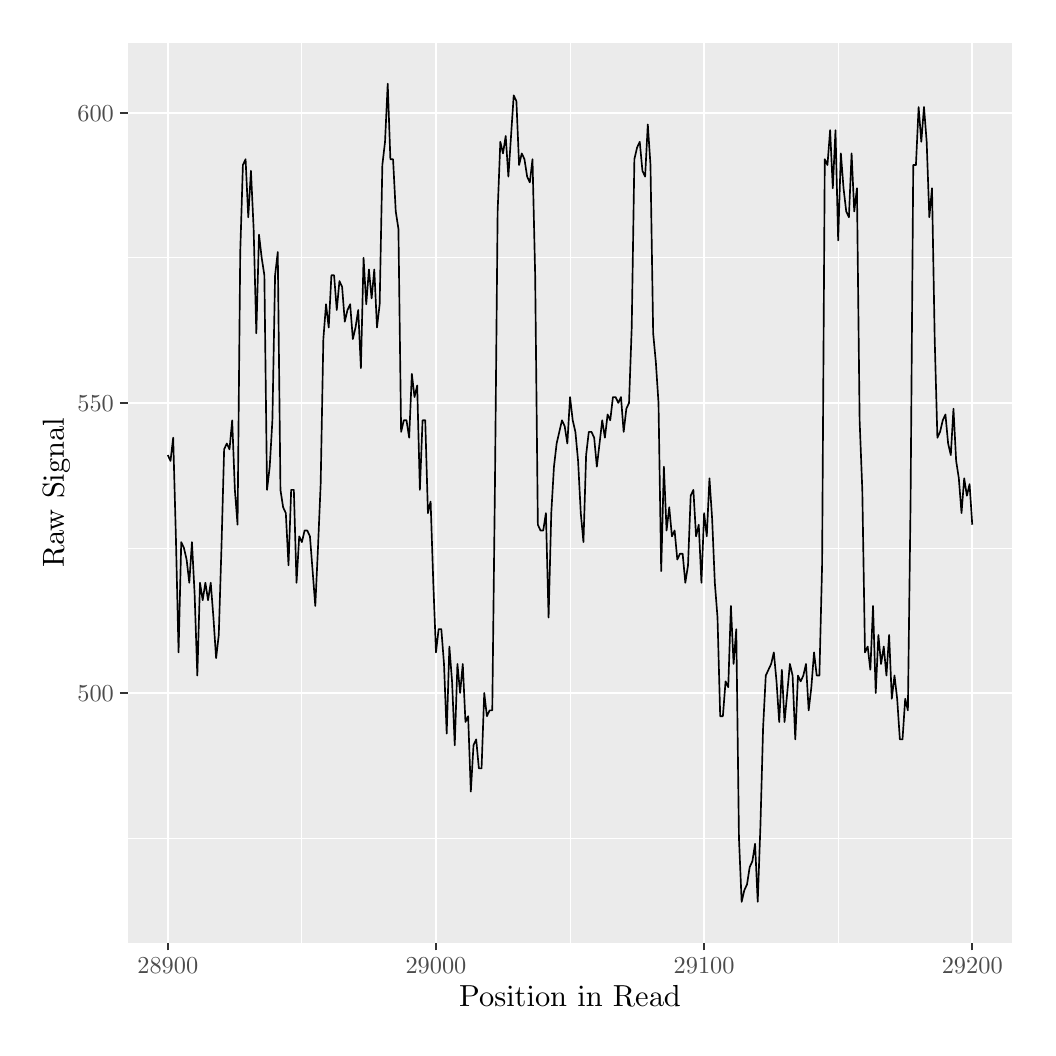
\begin{tikzpicture}[x=1pt,y=1pt]
\definecolor{fillColor}{RGB}{255,255,255}
\path[use as bounding box,fill=fillColor,fill opacity=0.00] (0,0) rectangle (361.35,361.35);
\begin{scope}
\path[clip] (  0.00,  0.00) rectangle (361.35,361.35);
\definecolor{drawColor}{RGB}{255,255,255}
\definecolor{fillColor}{RGB}{255,255,255}

\path[draw=drawColor,line width= 0.6pt,line join=round,line cap=round,fill=fillColor] (  0.00,  0.00) rectangle (361.35,361.35);
\end{scope}
\begin{scope}
\path[clip] ( 36.11, 30.69) rectangle (355.85,355.85);
\definecolor{fillColor}{gray}{0.92}

\path[fill=fillColor] ( 36.11, 30.69) rectangle (355.85,355.85);
\definecolor{drawColor}{RGB}{255,255,255}

\path[draw=drawColor,line width= 0.3pt,line join=round] ( 36.11, 68.53) --
	(355.85, 68.53);

\path[draw=drawColor,line width= 0.3pt,line join=round] ( 36.11,173.35) --
	(355.85,173.35);

\path[draw=drawColor,line width= 0.3pt,line join=round] ( 36.11,278.18) --
	(355.85,278.18);

\path[draw=drawColor,line width= 0.3pt,line join=round] ( 99.09, 30.69) --
	( 99.09,355.85);

\path[draw=drawColor,line width= 0.3pt,line join=round] (195.98, 30.69) --
	(195.98,355.85);

\path[draw=drawColor,line width= 0.3pt,line join=round] (292.87, 30.69) --
	(292.87,355.85);

\path[draw=drawColor,line width= 0.6pt,line join=round] ( 36.11,120.94) --
	(355.85,120.94);

\path[draw=drawColor,line width= 0.6pt,line join=round] ( 36.11,225.76) --
	(355.85,225.76);

\path[draw=drawColor,line width= 0.6pt,line join=round] ( 36.11,330.59) --
	(355.85,330.59);

\path[draw=drawColor,line width= 0.6pt,line join=round] ( 50.64, 30.69) --
	( 50.64,355.85);

\path[draw=drawColor,line width= 0.6pt,line join=round] (147.54, 30.69) --
	(147.54,355.85);

\path[draw=drawColor,line width= 0.6pt,line join=round] (244.43, 30.69) --
	(244.43,355.85);

\path[draw=drawColor,line width= 0.6pt,line join=round] (341.32, 30.69) --
	(341.32,355.85);
\definecolor{drawColor}{RGB}{0,0,0}

\path[draw=drawColor,line width= 0.6pt,line join=round] ( 50.64,206.90) --
	( 51.61,204.80) --
	( 52.58,213.18) --
	( 53.55,177.54) --
	( 54.52,135.61) --
	( 55.49,175.45) --
	( 56.46,173.35) --
	( 57.43,169.16) --
	( 58.40,160.77) --
	( 59.36,175.45) --
	( 60.33,156.58) --
	( 61.30,127.23) --
	( 62.27,160.77) --
	( 63.24,154.48) --
	( 64.21,160.77) --
	( 65.18,154.48) --
	( 66.15,160.77) --
	( 67.12,148.19) --
	( 68.09,133.52) --
	( 69.05,141.90) --
	( 70.02,173.35) --
	( 70.99,208.99) --
	( 71.96,211.09) --
	( 72.93,208.99) --
	( 73.90,219.47) --
	( 74.87,194.32) --
	( 75.84,181.74) --
	( 76.81,280.27) --
	( 77.77,311.72) --
	( 78.74,313.82) --
	( 79.71,292.85) --
	( 80.68,309.62) --
	( 81.65,288.66) --
	( 82.62,250.92) --
	( 83.59,286.56) --
	( 84.56,278.18) --
	( 85.53,271.89) --
	( 86.49,194.32) --
	( 87.46,202.70) --
	( 88.43,219.47) --
	( 89.40,271.89) --
	( 90.37,280.27) --
	( 91.34,194.32) --
	( 92.31,188.03) --
	( 93.28,185.93) --
	( 94.25,167.06) --
	( 95.21,194.32) --
	( 96.18,194.32) --
	( 97.15,160.77) --
	( 98.12,177.54) --
	( 99.09,175.45) --
	(100.06,179.64) --
	(101.03,179.64) --
	(102.00,177.54) --
	(102.97,164.97) --
	(103.93,152.39) --
	(104.90,173.35) --
	(105.87,196.41) --
	(106.84,248.82) --
	(107.81,261.40) --
	(108.78,253.02) --
	(109.75,271.89) --
	(110.72,271.89) --
	(111.69,259.31) --
	(112.65,269.79) --
	(113.62,267.69) --
	(114.59,255.11) --
	(115.56,259.31) --
	(116.53,261.40) --
	(117.50,248.82) --
	(118.47,253.02) --
	(119.44,259.31) --
	(120.41,238.34) --
	(121.37,278.18) --
	(122.34,261.40) --
	(123.31,273.98) --
	(124.28,263.50) --
	(125.25,273.98) --
	(126.22,253.02) --
	(127.19,261.40) --
	(128.16,311.72) --
	(129.13,320.11) --
	(130.10,341.07) --
	(131.06,313.82) --
	(132.03,313.82) --
	(133.00,294.95) --
	(133.97,288.66) --
	(134.94,215.28) --
	(135.91,219.47) --
	(136.88,219.47) --
	(137.85,213.18) --
	(138.82,236.25) --
	(139.78,227.86) --
	(140.75,232.05) --
	(141.72,194.32) --
	(142.69,219.47) --
	(143.66,219.47) --
	(144.63,185.93) --
	(145.60,190.12) --
	(146.57,160.77) --
	(147.54,135.61) --
	(148.50,144.00) --
	(149.47,144.00) --
	(150.44,131.42) --
	(151.41,106.26) --
	(152.38,137.71) --
	(153.35,125.13) --
	(154.32,102.07) --
	(155.29,131.42) --
	(156.26,120.94) --
	(157.22,131.42) --
	(158.19,110.46) --
	(159.16,112.55) --
	(160.13, 85.30) --
	(161.10,102.07) --
	(162.07,104.17) --
	(163.04, 93.69) --
	(164.01, 93.69) --
	(164.98,120.94) --
	(165.94,112.55) --
	(166.91,114.65) --
	(167.88,114.65) --
	(168.85,196.41) --
	(169.82,294.95) --
	(170.79,320.11) --
	(171.76,315.91) --
	(172.73,322.20) --
	(173.70,307.53) --
	(174.66,322.20) --
	(175.63,336.88) --
	(176.60,334.78) --
	(177.57,311.72) --
	(178.54,315.91) --
	(179.51,313.82) --
	(180.48,307.53) --
	(181.45,305.43) --
	(182.42,313.82) --
	(183.38,271.89) --
	(184.35,181.74) --
	(185.32,179.64) --
	(186.29,179.64) --
	(187.26,185.93) --
	(188.23,148.19) --
	(189.20,185.93) --
	(190.17,202.70) --
	(191.14,211.09) --
	(192.10,215.28) --
	(193.07,219.47) --
	(194.04,217.38) --
	(195.01,211.09) --
	(195.98,227.86) --
	(196.95,219.47) --
	(197.92,215.28) --
	(198.89,204.80) --
	(199.86,185.93) --
	(200.83,175.45) --
	(201.79,206.90) --
	(202.76,215.28) --
	(203.73,215.28) --
	(204.70,213.18) --
	(205.67,202.70) --
	(206.64,211.09) --
	(207.61,219.47) --
	(208.58,213.18) --
	(209.55,221.57) --
	(210.51,219.47) --
	(211.48,227.86) --
	(212.45,227.86) --
	(213.42,225.76) --
	(214.39,227.86) --
	(215.36,215.28) --
	(216.33,223.67) --
	(217.30,225.76) --
	(218.27,253.02) --
	(219.23,313.82) --
	(220.20,318.01) --
	(221.17,320.11) --
	(222.14,309.62) --
	(223.11,307.53) --
	(224.08,326.39) --
	(225.05,311.72) --
	(226.02,250.92) --
	(226.99,240.44) --
	(227.95,225.76) --
	(228.92,164.97) --
	(229.89,202.70) --
	(230.86,179.64) --
	(231.83,188.03) --
	(232.80,177.54) --
	(233.77,179.64) --
	(234.74,169.16) --
	(235.71,171.25) --
	(236.67,171.25) --
	(237.64,160.77) --
	(238.61,167.06) --
	(239.58,192.22) --
	(240.55,194.32) --
	(241.52,177.54) --
	(242.49,181.74) --
	(243.46,160.77) --
	(244.43,185.93) --
	(245.39,177.54) --
	(246.36,198.51) --
	(247.33,183.83) --
	(248.30,160.77) --
	(249.27,148.19) --
	(250.24,112.55) --
	(251.21,112.55) --
	(252.18,125.13) --
	(253.15,123.04) --
	(254.11,152.39) --
	(255.08,131.42) --
	(256.05,144.00) --
	(257.02, 68.53) --
	(257.99, 45.47) --
	(258.96, 49.66) --
	(259.93, 51.76) --
	(260.90, 58.04) --
	(261.87, 60.14) --
	(262.84, 66.43) --
	(263.80, 45.47) --
	(264.77, 72.72) --
	(265.74,108.36) --
	(266.71,127.23) --
	(267.68,129.33) --
	(268.65,131.42) --
	(269.62,135.61) --
	(270.59,125.13) --
	(271.56,110.46) --
	(272.52,129.33) --
	(273.49,110.46) --
	(274.46,120.94) --
	(275.43,131.42) --
	(276.40,127.23) --
	(277.37,104.17) --
	(278.34,127.23) --
	(279.31,125.13) --
	(280.28,127.23) --
	(281.24,131.42) --
	(282.21,114.65) --
	(283.18,123.04) --
	(284.15,135.61) --
	(285.12,127.23) --
	(286.09,127.23) --
	(287.06,167.06) --
	(288.03,313.82) --
	(289.00,311.72) --
	(289.96,324.30) --
	(290.93,303.33) --
	(291.90,324.30) --
	(292.87,284.46) --
	(293.84,315.91) --
	(294.81,303.33) --
	(295.78,294.95) --
	(296.75,292.85) --
	(297.72,315.91) --
	(298.68,294.95) --
	(299.65,303.33) --
	(300.62,219.47) --
	(301.59,194.32) --
	(302.56,135.61) --
	(303.53,137.71) --
	(304.50,129.33) --
	(305.47,152.39) --
	(306.44,120.94) --
	(307.40,141.90) --
	(308.37,131.42) --
	(309.34,137.71) --
	(310.31,127.23) --
	(311.28,141.90) --
	(312.25,118.84) --
	(313.22,127.23) --
	(314.19,118.84) --
	(315.16,104.17) --
	(316.12,104.17) --
	(317.09,118.84) --
	(318.06,114.65) --
	(319.03,190.12) --
	(320.00,311.72) --
	(320.97,311.72) --
	(321.94,332.68) --
	(322.91,320.11) --
	(323.88,332.68) --
	(324.85,320.11) --
	(325.81,292.85) --
	(326.78,303.33) --
	(327.75,248.82) --
	(328.72,213.18) --
	(329.69,215.28) --
	(330.66,219.47) --
	(331.63,221.57) --
	(332.60,211.09) --
	(333.57,206.90) --
	(334.53,223.67) --
	(335.50,204.80) --
	(336.47,198.51) --
	(337.44,185.93) --
	(338.41,198.51) --
	(339.38,192.22) --
	(340.35,196.41) --
	(341.32,181.74);
\end{scope}
\begin{scope}
\path[clip] (  0.00,  0.00) rectangle (361.35,361.35);
\definecolor{drawColor}{gray}{0.30}

\node[text=drawColor,anchor=base east,inner sep=0pt, outer sep=0pt, scale=  0.88] at ( 31.16,117.91) {500};

\node[text=drawColor,anchor=base east,inner sep=0pt, outer sep=0pt, scale=  0.88] at ( 31.16,222.73) {550};

\node[text=drawColor,anchor=base east,inner sep=0pt, outer sep=0pt, scale=  0.88] at ( 31.16,327.56) {600};
\end{scope}
\begin{scope}
\path[clip] (  0.00,  0.00) rectangle (361.35,361.35);
\definecolor{drawColor}{gray}{0.20}

\path[draw=drawColor,line width= 0.6pt,line join=round] ( 33.36,120.94) --
	( 36.11,120.94);

\path[draw=drawColor,line width= 0.6pt,line join=round] ( 33.36,225.76) --
	( 36.11,225.76);

\path[draw=drawColor,line width= 0.6pt,line join=round] ( 33.36,330.59) --
	( 36.11,330.59);
\end{scope}
\begin{scope}
\path[clip] (  0.00,  0.00) rectangle (361.35,361.35);
\definecolor{drawColor}{gray}{0.20}

\path[draw=drawColor,line width= 0.6pt,line join=round] ( 50.64, 27.94) --
	( 50.64, 30.69);

\path[draw=drawColor,line width= 0.6pt,line join=round] (147.54, 27.94) --
	(147.54, 30.69);

\path[draw=drawColor,line width= 0.6pt,line join=round] (244.43, 27.94) --
	(244.43, 30.69);

\path[draw=drawColor,line width= 0.6pt,line join=round] (341.32, 27.94) --
	(341.32, 30.69);
\end{scope}
\begin{scope}
\path[clip] (  0.00,  0.00) rectangle (361.35,361.35);
\definecolor{drawColor}{gray}{0.30}

\node[text=drawColor,anchor=base,inner sep=0pt, outer sep=0pt, scale=  0.88] at ( 50.64, 19.68) {28900};

\node[text=drawColor,anchor=base,inner sep=0pt, outer sep=0pt, scale=  0.88] at (147.54, 19.68) {29000};

\node[text=drawColor,anchor=base,inner sep=0pt, outer sep=0pt, scale=  0.88] at (244.43, 19.68) {29100};

\node[text=drawColor,anchor=base,inner sep=0pt, outer sep=0pt, scale=  0.88] at (341.32, 19.68) {29200};
\end{scope}
\begin{scope}
\path[clip] (  0.00,  0.00) rectangle (361.35,361.35);
\definecolor{drawColor}{RGB}{0,0,0}

\node[text=drawColor,anchor=base,inner sep=0pt, outer sep=0pt, scale=  1.10] at (195.98,  7.64) {Position in Read};
\end{scope}
\begin{scope}
\path[clip] (  0.00,  0.00) rectangle (361.35,361.35);
\definecolor{drawColor}{RGB}{0,0,0}

\node[text=drawColor,rotate= 90.00,anchor=base,inner sep=0pt, outer sep=0pt, scale=  1.10] at ( 13.08,193.27) {Raw Signal};
\end{scope}
\end{tikzpicture}

\caption{\label{fig:dna300-section}An example of 300 data points from a DNA
	section in the read with ID e9f08690-171f-476f-9119-5330d0290126. Notice
	the sudden transitions up and down (jumps and falls) between
	low-variance sections (flats).}
\end{figure}


The large majority of the data consists of DNA sections so any gains in
compression discovered by understanding this type of section should
result in the largest compression gains overall. Recall that the DNA sections of
nanopore signal data are characterised by many low-variance subsequences of 10--100
data points with steep transitions between them. See Figure
\ref{fig:dna300-section} for an example.

The problem with compressing the DNA sections is that there are a lot of
apparent irregularities as is expected with information saturated sensor data.
Furthermore, the zig-zag delta transformation is quite fast and produces a lower
entropy distribution which is readily compressible making it difficult to outperform.

\subsubsection{Separating the Jumps, Falls and Flats}

However, since we expect many low-variance sections with steep transitions
between them we can separate these two types of sections and compress each
separately. We will name the low-variance sections \textit{flats} and the
steep transitions up and down; \textit{jumps} and \textit{falls} respectively.
Since flats oscillate around some level, they should have small zig-zag deltas.
On the other hand, jumps and flats should have larger absolute deltas.

%Another useful observation is that the signal in a DNA
%section doesn't tend to stray far from its median -- that is, if it moves
%upwards it is more likely to move downwards next. This is clear if we refer back
%to the distribution of deltas (Figure \ref{fig:delta-hist}) which is symmetric
%except at the tails.

%However, we can take direct advantage of the signal's tendency to jump and fall
%between flatter sections.

For this reason, consider separating the read into two distributions: the
zig-zag deltas of flats, and the absolute deltas of jumps and falls. This should
benefit compression since each distribution will have its own unique properties
which benefit from different compression strategies. However, storing the
metadata necessary for the reconstruction of the read from each distribution may
be too high of a cost to incur any space saving.

Let's define a jump or fall as
\begin{itemize}
	\item a sequence of length $m\ge 2$ which is
	\item strictly increasing or decreasing respectively ($\forall i$ $\delta_i>0$ or $\forall i$ $\delta_i < 0$) with
	\item at least one absolute delta greater than some $\epsilon$ ($\exists i$ $s.t.$ $|\delta_i|>\epsilon$).
\end{itemize}

The idea with the third restriction is to actually capture sudden movements
rather than slowly increasing or decreasing sections, without which all non-zero
deltas would be labelled part of a jump or fall. The choice of which $\epsilon$
depends on the data and how much separation between flats and jumps/falls one
desires. For example, consider Figure \ref{fig:epsilon}. Here, each jump and fall
is coloured by the maximum epsilon for which it is still considered a jump or
fall. In other words, it is coloured by its largest absolute delta
($\max_i\{|\delta_i|\}$). Furthermore, it is labelled by this maximum if it is
greater than 20. From visual observation it appears that setting $\epsilon=24$
may define the jumps and falls as is expected. Figure \ref{fig:epsilon-25}
highlights the jumps and falls for $\epsilon=24$.

\begin{figure}
\centering
% Created by tikzDevice version 0.12.3.1 on 2022-10-19 16:29:31
% !TEX encoding = UTF-8 Unicode
\begin{tikzpicture}[x=1pt,y=1pt]
\definecolor{fillColor}{RGB}{255,255,255}
\path[use as bounding box,fill=fillColor,fill opacity=0.00] (0,0) rectangle (433.62,361.35);
\begin{scope}
\path[clip] (  0.00,  0.00) rectangle (433.62,361.35);
\definecolor{drawColor}{RGB}{255,255,255}
\definecolor{fillColor}{RGB}{255,255,255}

\path[draw=drawColor,line width= 0.6pt,line join=round,line cap=round,fill=fillColor] (  0.00,  0.00) rectangle (433.62,361.35);
\end{scope}
\begin{scope}
\path[clip] ( 36.11, 30.69) rectangle (357.55,355.85);
\definecolor{fillColor}{gray}{0.92}

\path[fill=fillColor] ( 36.11, 30.69) rectangle (357.55,355.85);
\definecolor{drawColor}{RGB}{255,255,255}

\path[draw=drawColor,line width= 0.3pt,line join=round] ( 36.11, 68.53) --
	(357.55, 68.53);

\path[draw=drawColor,line width= 0.3pt,line join=round] ( 36.11,173.35) --
	(357.55,173.35);

\path[draw=drawColor,line width= 0.3pt,line join=round] ( 36.11,278.18) --
	(357.55,278.18);

\path[draw=drawColor,line width= 0.3pt,line join=round] ( 99.42, 30.69) --
	( 99.42,355.85);

\path[draw=drawColor,line width= 0.3pt,line join=round] (196.83, 30.69) --
	(196.83,355.85);

\path[draw=drawColor,line width= 0.3pt,line join=round] (294.23, 30.69) --
	(294.23,355.85);

\path[draw=drawColor,line width= 0.6pt,line join=round] ( 36.11,120.94) --
	(357.55,120.94);

\path[draw=drawColor,line width= 0.6pt,line join=round] ( 36.11,225.76) --
	(357.55,225.76);

\path[draw=drawColor,line width= 0.6pt,line join=round] ( 36.11,330.59) --
	(357.55,330.59);

\path[draw=drawColor,line width= 0.6pt,line join=round] ( 50.72, 30.69) --
	( 50.72,355.85);

\path[draw=drawColor,line width= 0.6pt,line join=round] (148.13, 30.69) --
	(148.13,355.85);

\path[draw=drawColor,line width= 0.6pt,line join=round] (245.53, 30.69) --
	(245.53,355.85);

\path[draw=drawColor,line width= 0.6pt,line join=round] (342.94, 30.69) --
	(342.94,355.85);
\definecolor{drawColor}{RGB}{68,1,84}

\path[draw=drawColor,line width= 0.6pt,line join=round] ( 50.72,206.90) -- ( 51.70,204.80);
\definecolor{drawColor}{RGB}{69,21,95}

\path[draw=drawColor,line width= 0.6pt,line join=round] ( 51.70,204.80) -- ( 52.67,213.18);
\definecolor{drawColor}{RGB}{61,88,138}

\path[draw=drawColor,line width= 0.6pt,line join=round] ( 52.67,213.18) -- ( 53.64,177.54);

\path[draw=drawColor,line width= 0.6pt,line join=round] ( 53.64,177.54) -- ( 54.62,135.61);
\definecolor{drawColor}{RGB}{62,84,137}

\path[draw=drawColor,line width= 0.6pt,line join=round] ( 54.62,135.61) -- ( 55.59,175.45);
\definecolor{drawColor}{RGB}{69,21,95}

\path[draw=drawColor,line width= 0.6pt,line join=round] ( 55.59,175.45) -- ( 56.57,173.35);

\path[draw=drawColor,line width= 0.6pt,line join=round] ( 56.57,173.35) -- ( 57.54,169.16);

\path[draw=drawColor,line width= 0.6pt,line join=round] ( 57.54,169.16) -- ( 58.51,160.77);
\definecolor{drawColor}{RGB}{70,36,106}

\path[draw=drawColor,line width= 0.6pt,line join=round] ( 58.51,160.77) -- ( 59.49,175.45);
\definecolor{drawColor}{RGB}{66,65,132}

\path[draw=drawColor,line width= 0.6pt,line join=round] ( 59.49,175.45) -- ( 60.46,156.58);

\path[draw=drawColor,line width= 0.6pt,line join=round] ( 60.46,156.58) -- ( 61.44,127.23);
\definecolor{drawColor}{RGB}{64,73,136}

\path[draw=drawColor,line width= 0.6pt,line join=round] ( 61.44,127.23) -- ( 62.41,160.77);
\definecolor{drawColor}{RGB}{69,15,91}

\path[draw=drawColor,line width= 0.6pt,line join=round] ( 62.41,160.77) -- ( 63.38,154.48);

\path[draw=drawColor,line width= 0.6pt,line join=round] ( 63.38,154.48) -- ( 64.36,160.77);

\path[draw=drawColor,line width= 0.6pt,line join=round] ( 64.36,160.77) -- ( 65.33,154.48);

\path[draw=drawColor,line width= 0.6pt,line join=round] ( 65.33,154.48) -- ( 66.31,160.77);
\definecolor{drawColor}{RGB}{70,36,106}

\path[draw=drawColor,line width= 0.6pt,line join=round] ( 66.31,160.77) -- ( 67.28,148.19);

\path[draw=drawColor,line width= 0.6pt,line join=round] ( 67.28,148.19) -- ( 68.25,133.52);
\definecolor{drawColor}{RGB}{64,77,136}

\path[draw=drawColor,line width= 0.6pt,line join=round] ( 68.25,133.52) -- ( 69.23,141.90);

\path[draw=drawColor,line width= 0.6pt,line join=round] ( 69.23,141.90) -- ( 70.20,173.35);

\path[draw=drawColor,line width= 0.6pt,line join=round] ( 70.20,173.35) -- ( 71.18,208.99);

\path[draw=drawColor,line width= 0.6pt,line join=round] ( 71.18,208.99) -- ( 72.15,211.09);
\definecolor{drawColor}{RGB}{68,1,84}

\path[draw=drawColor,line width= 0.6pt,line join=round] ( 72.15,211.09) -- ( 73.13,208.99);
\definecolor{drawColor}{RGB}{70,27,98}

\path[draw=drawColor,line width= 0.6pt,line join=round] ( 73.13,208.99) -- ( 74.10,219.47);
\definecolor{drawColor}{RGB}{68,57,124}

\path[draw=drawColor,line width= 0.6pt,line join=round] ( 74.10,219.47) -- ( 75.07,194.32);

\path[draw=drawColor,line width= 0.6pt,line join=round] ( 75.07,194.32) -- ( 76.05,181.74);
\definecolor{drawColor}{RGB}{76,181,117}

\path[draw=drawColor,line width= 0.6pt,line join=round] ( 76.05,181.74) -- ( 77.02,280.27);

\path[draw=drawColor,line width= 0.6pt,line join=round] ( 77.02,280.27) -- ( 78.00,311.72);

\path[draw=drawColor,line width= 0.6pt,line join=round] ( 78.00,311.72) -- ( 78.97,313.82);
\definecolor{drawColor}{RGB}{69,49,117}

\path[draw=drawColor,line width= 0.6pt,line join=round] ( 78.97,313.82) -- ( 79.94,292.85);
\definecolor{drawColor}{RGB}{70,40,109}

\path[draw=drawColor,line width= 0.6pt,line join=round] ( 79.94,292.85) -- ( 80.92,309.62);
\definecolor{drawColor}{RGB}{63,80,137}

\path[draw=drawColor,line width= 0.6pt,line join=round] ( 80.92,309.62) -- ( 81.89,288.66);

\path[draw=drawColor,line width= 0.6pt,line join=round] ( 81.89,288.66) -- ( 82.87,250.92);
\definecolor{drawColor}{RGB}{64,77,136}

\path[draw=drawColor,line width= 0.6pt,line join=round] ( 82.87,250.92) -- ( 83.84,286.56);
\definecolor{drawColor}{RGB}{42,149,136}

\path[draw=drawColor,line width= 0.6pt,line join=round] ( 83.84,286.56) -- ( 84.81,278.18);

\path[draw=drawColor,line width= 0.6pt,line join=round] ( 84.81,278.18) -- ( 85.79,271.89);

\path[draw=drawColor,line width= 0.6pt,line join=round] ( 85.79,271.89) -- ( 86.76,194.32);
\definecolor{drawColor}{RGB}{53,107,140}

\path[draw=drawColor,line width= 0.6pt,line join=round] ( 86.76,194.32) -- ( 87.74,202.70);

\path[draw=drawColor,line width= 0.6pt,line join=round] ( 87.74,202.70) -- ( 88.71,219.47);

\path[draw=drawColor,line width= 0.6pt,line join=round] ( 88.71,219.47) -- ( 89.68,271.89);

\path[draw=drawColor,line width= 0.6pt,line join=round] ( 89.68,271.89) -- ( 90.66,280.27);
\definecolor{drawColor}{RGB}{37,163,133}

\path[draw=drawColor,line width= 0.6pt,line join=round] ( 90.66,280.27) -- ( 91.63,194.32);

\path[draw=drawColor,line width= 0.6pt,line join=round] ( 91.63,194.32) -- ( 92.61,188.03);

\path[draw=drawColor,line width= 0.6pt,line join=round] ( 92.61,188.03) -- ( 93.58,185.93);

\path[draw=drawColor,line width= 0.6pt,line join=round] ( 93.58,185.93) -- ( 94.55,167.06);
\definecolor{drawColor}{RGB}{67,61,128}

\path[draw=drawColor,line width= 0.6pt,line join=round] ( 94.55,167.06) -- ( 95.53,194.32);

\path[draw=drawColor,line width= 0.6pt,line join=round] ( 95.53,194.32) -- ( 96.50,194.32);
\definecolor{drawColor}{RGB}{64,73,136}

\path[draw=drawColor,line width= 0.6pt,line join=round] ( 96.50,194.32) -- ( 97.48,160.77);
\definecolor{drawColor}{RGB}{70,40,109}

\path[draw=drawColor,line width= 0.6pt,line join=round] ( 97.48,160.77) -- ( 98.45,177.54);
\definecolor{drawColor}{RGB}{68,1,84}

\path[draw=drawColor,line width= 0.6pt,line join=round] ( 98.45,177.54) -- ( 99.42,175.45);
\definecolor{drawColor}{RGB}{69,8,88}

\path[draw=drawColor,line width= 0.6pt,line join=round] ( 99.42,175.45) -- (100.40,179.64);

\path[draw=drawColor,line width= 0.6pt,line join=round] (100.40,179.64) -- (101.37,179.64);
\definecolor{drawColor}{RGB}{70,31,102}

\path[draw=drawColor,line width= 0.6pt,line join=round] (101.37,179.64) -- (102.35,177.54);

\path[draw=drawColor,line width= 0.6pt,line join=round] (102.35,177.54) -- (103.32,164.97);

\path[draw=drawColor,line width= 0.6pt,line join=round] (103.32,164.97) -- (104.29,152.39);
\definecolor{drawColor}{RGB}{53,107,140}

\path[draw=drawColor,line width= 0.6pt,line join=round] (104.29,152.39) -- (105.27,173.35);

\path[draw=drawColor,line width= 0.6pt,line join=round] (105.27,173.35) -- (106.24,196.41);

\path[draw=drawColor,line width= 0.6pt,line join=round] (106.24,196.41) -- (107.22,248.82);

\path[draw=drawColor,line width= 0.6pt,line join=round] (107.22,248.82) -- (108.19,261.40);
\definecolor{drawColor}{RGB}{69,21,95}

\path[draw=drawColor,line width= 0.6pt,line join=round] (108.19,261.40) -- (109.17,253.02);
\definecolor{drawColor}{RGB}{69,45,113}

\path[draw=drawColor,line width= 0.6pt,line join=round] (109.17,253.02) -- (110.14,271.89);

\path[draw=drawColor,line width= 0.6pt,line join=round] (110.14,271.89) -- (111.11,271.89);
\definecolor{drawColor}{RGB}{70,31,102}

\path[draw=drawColor,line width= 0.6pt,line join=round] (111.11,271.89) -- (112.09,259.31);
\definecolor{drawColor}{RGB}{70,27,98}

\path[draw=drawColor,line width= 0.6pt,line join=round] (112.09,259.31) -- (113.06,269.79);
\definecolor{drawColor}{RGB}{70,31,102}

\path[draw=drawColor,line width= 0.6pt,line join=round] (113.06,269.79) -- (114.04,267.69);

\path[draw=drawColor,line width= 0.6pt,line join=round] (114.04,267.69) -- (115.01,255.11);
\definecolor{drawColor}{RGB}{69,8,88}

\path[draw=drawColor,line width= 0.6pt,line join=round] (115.01,255.11) -- (115.98,259.31);

\path[draw=drawColor,line width= 0.6pt,line join=round] (115.98,259.31) -- (116.96,261.40);
\definecolor{drawColor}{RGB}{70,31,102}

\path[draw=drawColor,line width= 0.6pt,line join=round] (116.96,261.40) -- (117.93,248.82);
\definecolor{drawColor}{RGB}{69,15,91}

\path[draw=drawColor,line width= 0.6pt,line join=round] (117.93,248.82) -- (118.91,253.02);

\path[draw=drawColor,line width= 0.6pt,line join=round] (118.91,253.02) -- (119.88,259.31);
\definecolor{drawColor}{RGB}{69,49,117}

\path[draw=drawColor,line width= 0.6pt,line join=round] (119.88,259.31) -- (120.85,238.34);
\definecolor{drawColor}{RGB}{62,84,137}

\path[draw=drawColor,line width= 0.6pt,line join=round] (120.85,238.34) -- (121.83,278.18);
\definecolor{drawColor}{RGB}{70,40,109}

\path[draw=drawColor,line width= 0.6pt,line join=round] (121.83,278.18) -- (122.80,261.40);
\definecolor{drawColor}{RGB}{70,31,102}

\path[draw=drawColor,line width= 0.6pt,line join=round] (122.80,261.40) -- (123.78,273.98);
\definecolor{drawColor}{RGB}{70,27,98}

\path[draw=drawColor,line width= 0.6pt,line join=round] (123.78,273.98) -- (124.75,263.50);

\path[draw=drawColor,line width= 0.6pt,line join=round] (124.75,263.50) -- (125.72,273.98);
\definecolor{drawColor}{RGB}{69,49,117}

\path[draw=drawColor,line width= 0.6pt,line join=round] (125.72,273.98) -- (126.70,253.02);
\definecolor{drawColor}{RGB}{55,103,140}

\path[draw=drawColor,line width= 0.6pt,line join=round] (126.70,253.02) -- (127.67,261.40);

\path[draw=drawColor,line width= 0.6pt,line join=round] (127.67,261.40) -- (128.65,311.72);

\path[draw=drawColor,line width= 0.6pt,line join=round] (128.65,311.72) -- (129.62,320.11);

\path[draw=drawColor,line width= 0.6pt,line join=round] (129.62,320.11) -- (130.59,341.07);
\definecolor{drawColor}{RGB}{67,61,128}

\path[draw=drawColor,line width= 0.6pt,line join=round] (130.59,341.07) -- (131.57,313.82);

\path[draw=drawColor,line width= 0.6pt,line join=round] (131.57,313.82) -- (132.54,313.82);
\definecolor{drawColor}{RGB}{43,142,138}

\path[draw=drawColor,line width= 0.6pt,line join=round] (132.54,313.82) -- (133.52,294.95);

\path[draw=drawColor,line width= 0.6pt,line join=round] (133.52,294.95) -- (134.49,288.66);

\path[draw=drawColor,line width= 0.6pt,line join=round] (134.49,288.66) -- (135.46,215.28);
\definecolor{drawColor}{RGB}{69,8,88}

\path[draw=drawColor,line width= 0.6pt,line join=round] (135.46,215.28) -- (136.44,219.47);

\path[draw=drawColor,line width= 0.6pt,line join=round] (136.44,219.47) -- (137.41,219.47);
\definecolor{drawColor}{RGB}{69,15,91}

\path[draw=drawColor,line width= 0.6pt,line join=round] (137.41,219.47) -- (138.39,213.18);
\definecolor{drawColor}{RGB}{68,53,121}

\path[draw=drawColor,line width= 0.6pt,line join=round] (138.39,213.18) -- (139.36,236.25);
\definecolor{drawColor}{RGB}{69,21,95}

\path[draw=drawColor,line width= 0.6pt,line join=round] (139.36,236.25) -- (140.33,227.86);
\definecolor{drawColor}{RGB}{69,8,88}

\path[draw=drawColor,line width= 0.6pt,line join=round] (140.33,227.86) -- (141.31,232.05);
\definecolor{drawColor}{RGB}{63,80,137}

\path[draw=drawColor,line width= 0.6pt,line join=round] (141.31,232.05) -- (142.28,194.32);
\definecolor{drawColor}{RGB}{68,57,124}

\path[draw=drawColor,line width= 0.6pt,line join=round] (142.28,194.32) -- (143.26,219.47);

\path[draw=drawColor,line width= 0.6pt,line join=round] (143.26,219.47) -- (144.23,219.47);
\definecolor{drawColor}{RGB}{64,73,136}

\path[draw=drawColor,line width= 0.6pt,line join=round] (144.23,219.47) -- (145.20,185.93);
\definecolor{drawColor}{RGB}{69,8,88}

\path[draw=drawColor,line width= 0.6pt,line join=round] (145.20,185.93) -- (146.18,190.12);
\definecolor{drawColor}{RGB}{66,65,132}

\path[draw=drawColor,line width= 0.6pt,line join=round] (146.18,190.12) -- (147.15,160.77);

\path[draw=drawColor,line width= 0.6pt,line join=round] (147.15,160.77) -- (148.13,135.61);
\definecolor{drawColor}{RGB}{69,21,95}

\path[draw=drawColor,line width= 0.6pt,line join=round] (148.13,135.61) -- (149.10,144.00);

\path[draw=drawColor,line width= 0.6pt,line join=round] (149.10,144.00) -- (150.08,144.00);
\definecolor{drawColor}{RGB}{68,57,124}

\path[draw=drawColor,line width= 0.6pt,line join=round] (150.08,144.00) -- (151.05,131.42);

\path[draw=drawColor,line width= 0.6pt,line join=round] (151.05,131.42) -- (152.02,106.26);
\definecolor{drawColor}{RGB}{65,69,135}

\path[draw=drawColor,line width= 0.6pt,line join=round] (152.02,106.26) -- (153.00,137.71);
\definecolor{drawColor}{RGB}{68,53,121}

\path[draw=drawColor,line width= 0.6pt,line join=round] (153.00,137.71) -- (153.97,125.13);

\path[draw=drawColor,line width= 0.6pt,line join=round] (153.97,125.13) -- (154.95,102.07);
\definecolor{drawColor}{RGB}{66,65,132}

\path[draw=drawColor,line width= 0.6pt,line join=round] (154.95,102.07) -- (155.92,131.42);
\definecolor{drawColor}{RGB}{70,27,98}

\path[draw=drawColor,line width= 0.6pt,line join=round] (155.92,131.42) -- (156.89,120.94);

\path[draw=drawColor,line width= 0.6pt,line join=round] (156.89,120.94) -- (157.87,131.42);
\definecolor{drawColor}{RGB}{69,49,117}

\path[draw=drawColor,line width= 0.6pt,line join=round] (157.87,131.42) -- (158.84,110.46);
\definecolor{drawColor}{RGB}{68,1,84}

\path[draw=drawColor,line width= 0.6pt,line join=round] (158.84,110.46) -- (159.82,112.55);
\definecolor{drawColor}{RGB}{67,61,128}

\path[draw=drawColor,line width= 0.6pt,line join=round] (159.82,112.55) -- (160.79, 85.30);
\definecolor{drawColor}{RGB}{70,40,109}

\path[draw=drawColor,line width= 0.6pt,line join=round] (160.79, 85.30) -- (161.76,102.07);

\path[draw=drawColor,line width= 0.6pt,line join=round] (161.76,102.07) -- (162.74,104.17);
\definecolor{drawColor}{RGB}{70,27,98}

\path[draw=drawColor,line width= 0.6pt,line join=round] (162.74,104.17) -- (163.71, 93.69);

\path[draw=drawColor,line width= 0.6pt,line join=round] (163.71, 93.69) -- (164.69, 93.69);
\definecolor{drawColor}{RGB}{67,61,128}

\path[draw=drawColor,line width= 0.6pt,line join=round] (164.69, 93.69) -- (165.66,120.94);
\definecolor{drawColor}{RGB}{69,21,95}

\path[draw=drawColor,line width= 0.6pt,line join=round] (165.66,120.94) -- (166.63,112.55);
\definecolor{drawColor}{RGB}{68,1,84}

\path[draw=drawColor,line width= 0.6pt,line join=round] (166.63,112.55) -- (167.61,114.65);

\path[draw=drawColor,line width= 0.6pt,line join=round] (167.61,114.65) -- (168.58,114.65);
\definecolor{drawColor}{RGB}{76,181,117}

\path[draw=drawColor,line width= 0.6pt,line join=round] (168.58,114.65) -- (169.56,196.41);

\path[draw=drawColor,line width= 0.6pt,line join=round] (169.56,196.41) -- (170.53,294.95);

\path[draw=drawColor,line width= 0.6pt,line join=round] (170.53,294.95) -- (171.50,320.11);
\definecolor{drawColor}{RGB}{69,8,88}

\path[draw=drawColor,line width= 0.6pt,line join=round] (171.50,320.11) -- (172.48,315.91);
\definecolor{drawColor}{RGB}{69,15,91}

\path[draw=drawColor,line width= 0.6pt,line join=round] (172.48,315.91) -- (173.45,322.20);
\definecolor{drawColor}{RGB}{70,36,106}

\path[draw=drawColor,line width= 0.6pt,line join=round] (173.45,322.20) -- (174.43,307.53);

\path[draw=drawColor,line width= 0.6pt,line join=round] (174.43,307.53) -- (175.40,322.20);

\path[draw=drawColor,line width= 0.6pt,line join=round] (175.40,322.20) -- (176.37,336.88);
\definecolor{drawColor}{RGB}{68,53,121}

\path[draw=drawColor,line width= 0.6pt,line join=round] (176.37,336.88) -- (177.35,334.78);

\path[draw=drawColor,line width= 0.6pt,line join=round] (177.35,334.78) -- (178.32,311.72);
\definecolor{drawColor}{RGB}{69,8,88}

\path[draw=drawColor,line width= 0.6pt,line join=round] (178.32,311.72) -- (179.30,315.91);
\definecolor{drawColor}{RGB}{69,15,91}

\path[draw=drawColor,line width= 0.6pt,line join=round] (179.30,315.91) -- (180.27,313.82);

\path[draw=drawColor,line width= 0.6pt,line join=round] (180.27,313.82) -- (181.24,307.53);

\path[draw=drawColor,line width= 0.6pt,line join=round] (181.24,307.53) -- (182.22,305.43);
\definecolor{drawColor}{RGB}{69,21,95}

\path[draw=drawColor,line width= 0.6pt,line join=round] (182.22,305.43) -- (183.19,313.82);
\definecolor{drawColor}{RGB}{42,170,130}

\path[draw=drawColor,line width= 0.6pt,line join=round] (183.19,313.82) -- (184.17,271.89);

\path[draw=drawColor,line width= 0.6pt,line join=round] (184.17,271.89) -- (185.14,181.74);

\path[draw=drawColor,line width= 0.6pt,line join=round] (185.14,181.74) -- (186.12,179.64);

\path[draw=drawColor,line width= 0.6pt,line join=round] (186.12,179.64) -- (187.09,179.64);
\definecolor{drawColor}{RGB}{69,15,91}

\path[draw=drawColor,line width= 0.6pt,line join=round] (187.09,179.64) -- (188.06,185.93);
\definecolor{drawColor}{RGB}{63,80,137}

\path[draw=drawColor,line width= 0.6pt,line join=round] (188.06,185.93) -- (189.04,148.19);

\path[draw=drawColor,line width= 0.6pt,line join=round] (189.04,148.19) -- (190.01,185.93);

\path[draw=drawColor,line width= 0.6pt,line join=round] (190.01,185.93) -- (190.99,202.70);

\path[draw=drawColor,line width= 0.6pt,line join=round] (190.99,202.70) -- (191.96,211.09);

\path[draw=drawColor,line width= 0.6pt,line join=round] (191.96,211.09) -- (192.93,215.28);

\path[draw=drawColor,line width= 0.6pt,line join=round] (192.93,215.28) -- (193.91,219.47);
\definecolor{drawColor}{RGB}{69,15,91}

\path[draw=drawColor,line width= 0.6pt,line join=round] (193.91,219.47) -- (194.88,217.38);

\path[draw=drawColor,line width= 0.6pt,line join=round] (194.88,217.38) -- (195.86,211.09);
\definecolor{drawColor}{RGB}{70,40,109}

\path[draw=drawColor,line width= 0.6pt,line join=round] (195.86,211.09) -- (196.83,227.86);
\definecolor{drawColor}{RGB}{69,45,113}

\path[draw=drawColor,line width= 0.6pt,line join=round] (196.83,227.86) -- (197.80,219.47);

\path[draw=drawColor,line width= 0.6pt,line join=round] (197.80,219.47) -- (198.78,215.28);

\path[draw=drawColor,line width= 0.6pt,line join=round] (198.78,215.28) -- (199.75,204.80);

\path[draw=drawColor,line width= 0.6pt,line join=round] (199.75,204.80) -- (200.73,185.93);

\path[draw=drawColor,line width= 0.6pt,line join=round] (200.73,185.93) -- (201.70,175.45);
\definecolor{drawColor}{RGB}{65,69,135}

\path[draw=drawColor,line width= 0.6pt,line join=round] (201.70,175.45) -- (202.67,206.90);

\path[draw=drawColor,line width= 0.6pt,line join=round] (202.67,206.90) -- (203.65,215.28);

\path[draw=drawColor,line width= 0.6pt,line join=round] (203.65,215.28) -- (204.62,215.28);
\definecolor{drawColor}{RGB}{70,27,98}

\path[draw=drawColor,line width= 0.6pt,line join=round] (204.62,215.28) -- (205.60,213.18);

\path[draw=drawColor,line width= 0.6pt,line join=round] (205.60,213.18) -- (206.57,202.70);
\definecolor{drawColor}{RGB}{69,21,95}

\path[draw=drawColor,line width= 0.6pt,line join=round] (206.57,202.70) -- (207.54,211.09);

\path[draw=drawColor,line width= 0.6pt,line join=round] (207.54,211.09) -- (208.52,219.47);
\definecolor{drawColor}{RGB}{69,15,91}

\path[draw=drawColor,line width= 0.6pt,line join=round] (208.52,219.47) -- (209.49,213.18);
\definecolor{drawColor}{RGB}{69,21,95}

\path[draw=drawColor,line width= 0.6pt,line join=round] (209.49,213.18) -- (210.47,221.57);
\definecolor{drawColor}{RGB}{68,1,84}

\path[draw=drawColor,line width= 0.6pt,line join=round] (210.47,221.57) -- (211.44,219.47);
\definecolor{drawColor}{RGB}{69,21,95}

\path[draw=drawColor,line width= 0.6pt,line join=round] (211.44,219.47) -- (212.41,227.86);

\path[draw=drawColor,line width= 0.6pt,line join=round] (212.41,227.86) -- (213.39,227.86);
\definecolor{drawColor}{RGB}{68,1,84}

\path[draw=drawColor,line width= 0.6pt,line join=round] (213.39,227.86) -- (214.36,225.76);

\path[draw=drawColor,line width= 0.6pt,line join=round] (214.36,225.76) -- (215.34,227.86);
\definecolor{drawColor}{RGB}{70,31,102}

\path[draw=drawColor,line width= 0.6pt,line join=round] (215.34,227.86) -- (216.31,215.28);
\definecolor{drawColor}{RGB}{42,121,142}

\path[draw=drawColor,line width= 0.6pt,line join=round] (216.31,215.28) -- (217.28,223.67);

\path[draw=drawColor,line width= 0.6pt,line join=round] (217.28,223.67) -- (218.26,225.76);

\path[draw=drawColor,line width= 0.6pt,line join=round] (218.26,225.76) -- (219.23,253.02);

\path[draw=drawColor,line width= 0.6pt,line join=round] (219.23,253.02) -- (220.21,313.82);

\path[draw=drawColor,line width= 0.6pt,line join=round] (220.21,313.82) -- (221.18,318.01);

\path[draw=drawColor,line width= 0.6pt,line join=round] (221.18,318.01) -- (222.16,320.11);
\definecolor{drawColor}{RGB}{70,27,98}

\path[draw=drawColor,line width= 0.6pt,line join=round] (222.16,320.11) -- (223.13,309.62);

\path[draw=drawColor,line width= 0.6pt,line join=round] (223.13,309.62) -- (224.10,307.53);
\definecolor{drawColor}{RGB}{69,45,113}

\path[draw=drawColor,line width= 0.6pt,line join=round] (224.10,307.53) -- (225.08,326.39);
\definecolor{drawColor}{RGB}{42,121,142}

\path[draw=drawColor,line width= 0.6pt,line join=round] (225.08,326.39) -- (226.05,311.72);

\path[draw=drawColor,line width= 0.6pt,line join=round] (226.05,311.72) -- (227.03,250.92);

\path[draw=drawColor,line width= 0.6pt,line join=round] (227.03,250.92) -- (228.00,240.44);

\path[draw=drawColor,line width= 0.6pt,line join=round] (228.00,240.44) -- (228.97,225.76);

\path[draw=drawColor,line width= 0.6pt,line join=round] (228.97,225.76) -- (229.95,164.97);
\definecolor{drawColor}{RGB}{63,80,137}

\path[draw=drawColor,line width= 0.6pt,line join=round] (229.95,164.97) -- (230.92,202.70);
\definecolor{drawColor}{RGB}{68,53,121}

\path[draw=drawColor,line width= 0.6pt,line join=round] (230.92,202.70) -- (231.90,179.64);
\definecolor{drawColor}{RGB}{69,21,95}

\path[draw=drawColor,line width= 0.6pt,line join=round] (231.90,179.64) -- (232.87,188.03);
\definecolor{drawColor}{RGB}{70,27,98}

\path[draw=drawColor,line width= 0.6pt,line join=round] (232.87,188.03) -- (233.84,177.54);
\definecolor{drawColor}{RGB}{68,1,84}

\path[draw=drawColor,line width= 0.6pt,line join=round] (233.84,177.54) -- (234.82,179.64);
\definecolor{drawColor}{RGB}{70,27,98}

\path[draw=drawColor,line width= 0.6pt,line join=round] (234.82,179.64) -- (235.79,169.16);
\definecolor{drawColor}{RGB}{68,1,84}

\path[draw=drawColor,line width= 0.6pt,line join=round] (235.79,169.16) -- (236.77,171.25);

\path[draw=drawColor,line width= 0.6pt,line join=round] (236.77,171.25) -- (237.74,171.25);
\definecolor{drawColor}{RGB}{70,27,98}

\path[draw=drawColor,line width= 0.6pt,line join=round] (237.74,171.25) -- (238.71,160.77);
\definecolor{drawColor}{RGB}{68,57,124}

\path[draw=drawColor,line width= 0.6pt,line join=round] (238.71,160.77) -- (239.69,167.06);

\path[draw=drawColor,line width= 0.6pt,line join=round] (239.69,167.06) -- (240.66,192.22);

\path[draw=drawColor,line width= 0.6pt,line join=round] (240.66,192.22) -- (241.64,194.32);
\definecolor{drawColor}{RGB}{70,40,109}

\path[draw=drawColor,line width= 0.6pt,line join=round] (241.64,194.32) -- (242.61,177.54);
\definecolor{drawColor}{RGB}{69,8,88}

\path[draw=drawColor,line width= 0.6pt,line join=round] (242.61,177.54) -- (243.58,181.74);
\definecolor{drawColor}{RGB}{69,49,117}

\path[draw=drawColor,line width= 0.6pt,line join=round] (243.58,181.74) -- (244.56,160.77);
\definecolor{drawColor}{RGB}{68,57,124}

\path[draw=drawColor,line width= 0.6pt,line join=round] (244.56,160.77) -- (245.53,185.93);
\definecolor{drawColor}{RGB}{69,21,95}

\path[draw=drawColor,line width= 0.6pt,line join=round] (245.53,185.93) -- (246.51,177.54);
\definecolor{drawColor}{RGB}{69,49,117}

\path[draw=drawColor,line width= 0.6pt,line join=round] (246.51,177.54) -- (247.48,198.51);
\definecolor{drawColor}{RGB}{64,77,136}

\path[draw=drawColor,line width= 0.6pt,line join=round] (247.48,198.51) -- (248.45,183.83);

\path[draw=drawColor,line width= 0.6pt,line join=round] (248.45,183.83) -- (249.43,160.77);

\path[draw=drawColor,line width= 0.6pt,line join=round] (249.43,160.77) -- (250.40,148.19);

\path[draw=drawColor,line width= 0.6pt,line join=round] (250.40,148.19) -- (251.38,112.55);

\path[draw=drawColor,line width= 0.6pt,line join=round] (251.38,112.55) -- (252.35,112.55);
\definecolor{drawColor}{RGB}{70,31,102}

\path[draw=drawColor,line width= 0.6pt,line join=round] (252.35,112.55) -- (253.32,125.13);
\definecolor{drawColor}{RGB}{68,1,84}

\path[draw=drawColor,line width= 0.6pt,line join=round] (253.32,125.13) -- (254.30,123.04);
\definecolor{drawColor}{RGB}{66,65,132}

\path[draw=drawColor,line width= 0.6pt,line join=round] (254.30,123.04) -- (255.27,152.39);
\definecolor{drawColor}{RGB}{69,49,117}

\path[draw=drawColor,line width= 0.6pt,line join=round] (255.27,152.39) -- (256.25,131.42);
\definecolor{drawColor}{RGB}{70,31,102}

\path[draw=drawColor,line width= 0.6pt,line join=round] (256.25,131.42) -- (257.22,144.00);
\definecolor{drawColor}{RGB}{43,145,137}

\path[draw=drawColor,line width= 0.6pt,line join=round] (257.22,144.00) -- (258.19, 68.53);

\path[draw=drawColor,line width= 0.6pt,line join=round] (258.19, 68.53) -- (259.17, 45.47);
\definecolor{drawColor}{RGB}{69,15,91}

\path[draw=drawColor,line width= 0.6pt,line join=round] (259.17, 45.47) -- (260.14, 49.66);

\path[draw=drawColor,line width= 0.6pt,line join=round] (260.14, 49.66) -- (261.12, 51.76);

\path[draw=drawColor,line width= 0.6pt,line join=round] (261.12, 51.76) -- (262.09, 58.04);

\path[draw=drawColor,line width= 0.6pt,line join=round] (262.09, 58.04) -- (263.07, 60.14);

\path[draw=drawColor,line width= 0.6pt,line join=round] (263.07, 60.14) -- (264.04, 66.43);
\definecolor{drawColor}{RGB}{69,49,117}

\path[draw=drawColor,line width= 0.6pt,line join=round] (264.04, 66.43) -- (265.01, 45.47);
\definecolor{drawColor}{RGB}{64,77,136}

\path[draw=drawColor,line width= 0.6pt,line join=round] (265.01, 45.47) -- (265.99, 72.72);

\path[draw=drawColor,line width= 0.6pt,line join=round] (265.99, 72.72) -- (266.96,108.36);

\path[draw=drawColor,line width= 0.6pt,line join=round] (266.96,108.36) -- (267.94,127.23);

\path[draw=drawColor,line width= 0.6pt,line join=round] (267.94,127.23) -- (268.91,129.33);

\path[draw=drawColor,line width= 0.6pt,line join=round] (268.91,129.33) -- (269.88,131.42);

\path[draw=drawColor,line width= 0.6pt,line join=round] (269.88,131.42) -- (270.86,135.61);
\definecolor{drawColor}{RGB}{70,36,106}

\path[draw=drawColor,line width= 0.6pt,line join=round] (270.86,135.61) -- (271.83,125.13);

\path[draw=drawColor,line width= 0.6pt,line join=round] (271.83,125.13) -- (272.81,110.46);
\definecolor{drawColor}{RGB}{69,45,113}

\path[draw=drawColor,line width= 0.6pt,line join=round] (272.81,110.46) -- (273.78,129.33);

\path[draw=drawColor,line width= 0.6pt,line join=round] (273.78,129.33) -- (274.75,110.46);
\definecolor{drawColor}{RGB}{70,27,98}

\path[draw=drawColor,line width= 0.6pt,line join=round] (274.75,110.46) -- (275.73,120.94);

\path[draw=drawColor,line width= 0.6pt,line join=round] (275.73,120.94) -- (276.70,131.42);
\definecolor{drawColor}{RGB}{68,53,121}

\path[draw=drawColor,line width= 0.6pt,line join=round] (276.70,131.42) -- (277.68,127.23);

\path[draw=drawColor,line width= 0.6pt,line join=round] (277.68,127.23) -- (278.65,104.17);

\path[draw=drawColor,line width= 0.6pt,line join=round] (278.65,104.17) -- (279.62,127.23);
\definecolor{drawColor}{RGB}{68,1,84}

\path[draw=drawColor,line width= 0.6pt,line join=round] (279.62,127.23) -- (280.60,125.13);
\definecolor{drawColor}{RGB}{69,8,88}

\path[draw=drawColor,line width= 0.6pt,line join=round] (280.60,125.13) -- (281.57,127.23);

\path[draw=drawColor,line width= 0.6pt,line join=round] (281.57,127.23) -- (282.55,131.42);
\definecolor{drawColor}{RGB}{70,40,109}

\path[draw=drawColor,line width= 0.6pt,line join=round] (282.55,131.42) -- (283.52,114.65);
\definecolor{drawColor}{RGB}{70,31,102}

\path[draw=drawColor,line width= 0.6pt,line join=round] (283.52,114.65) -- (284.49,123.04);

\path[draw=drawColor,line width= 0.6pt,line join=round] (284.49,123.04) -- (285.47,135.61);
\definecolor{drawColor}{RGB}{69,21,95}

\path[draw=drawColor,line width= 0.6pt,line join=round] (285.47,135.61) -- (286.44,127.23);

\path[draw=drawColor,line width= 0.6pt,line join=round] (286.44,127.23) -- (287.42,127.23);
\definecolor{drawColor}{RGB}{253,231,37}

\path[draw=drawColor,line width= 0.6pt,line join=round] (287.42,127.23) -- (288.39,167.06);

\path[draw=drawColor,line width= 0.6pt,line join=round] (288.39,167.06) -- (289.36,313.82);
\definecolor{drawColor}{RGB}{68,1,84}

\path[draw=drawColor,line width= 0.6pt,line join=round] (289.36,313.82) -- (290.34,311.72);
\definecolor{drawColor}{RGB}{70,31,102}

\path[draw=drawColor,line width= 0.6pt,line join=round] (290.34,311.72) -- (291.31,324.30);
\definecolor{drawColor}{RGB}{69,49,117}

\path[draw=drawColor,line width= 0.6pt,line join=round] (291.31,324.30) -- (292.29,303.33);

\path[draw=drawColor,line width= 0.6pt,line join=round] (292.29,303.33) -- (293.26,324.30);
\definecolor{drawColor}{RGB}{62,84,137}

\path[draw=drawColor,line width= 0.6pt,line join=round] (293.26,324.30) -- (294.23,284.46);
\definecolor{drawColor}{RGB}{65,69,135}

\path[draw=drawColor,line width= 0.6pt,line join=round] (294.23,284.46) -- (295.21,315.91);
\definecolor{drawColor}{RGB}{70,31,102}

\path[draw=drawColor,line width= 0.6pt,line join=round] (295.21,315.91) -- (296.18,303.33);

\path[draw=drawColor,line width= 0.6pt,line join=round] (296.18,303.33) -- (297.16,294.95);

\path[draw=drawColor,line width= 0.6pt,line join=round] (297.16,294.95) -- (298.13,292.85);
\definecolor{drawColor}{RGB}{68,53,121}

\path[draw=drawColor,line width= 0.6pt,line join=round] (298.13,292.85) -- (299.11,315.91);
\definecolor{drawColor}{RGB}{69,49,117}

\path[draw=drawColor,line width= 0.6pt,line join=round] (299.11,315.91) -- (300.08,294.95);
\definecolor{drawColor}{RGB}{69,21,95}

\path[draw=drawColor,line width= 0.6pt,line join=round] (300.08,294.95) -- (301.05,303.33);
\definecolor{drawColor}{RGB}{39,160,134}

\path[draw=drawColor,line width= 0.6pt,line join=round] (301.05,303.33) -- (302.03,219.47);

\path[draw=drawColor,line width= 0.6pt,line join=round] (302.03,219.47) -- (303.00,194.32);

\path[draw=drawColor,line width= 0.6pt,line join=round] (303.00,194.32) -- (303.98,135.61);
\definecolor{drawColor}{RGB}{68,1,84}

\path[draw=drawColor,line width= 0.6pt,line join=round] (303.98,135.61) -- (304.95,137.71);
\definecolor{drawColor}{RGB}{69,21,95}

\path[draw=drawColor,line width= 0.6pt,line join=round] (304.95,137.71) -- (305.92,129.33);
\definecolor{drawColor}{RGB}{68,53,121}

\path[draw=drawColor,line width= 0.6pt,line join=round] (305.92,129.33) -- (306.90,152.39);
\definecolor{drawColor}{RGB}{65,69,135}

\path[draw=drawColor,line width= 0.6pt,line join=round] (306.90,152.39) -- (307.87,120.94);
\definecolor{drawColor}{RGB}{69,49,117}

\path[draw=drawColor,line width= 0.6pt,line join=round] (307.87,120.94) -- (308.85,141.90);
\definecolor{drawColor}{RGB}{70,27,98}

\path[draw=drawColor,line width= 0.6pt,line join=round] (308.85,141.90) -- (309.82,131.42);
\definecolor{drawColor}{RGB}{69,15,91}

\path[draw=drawColor,line width= 0.6pt,line join=round] (309.82,131.42) -- (310.79,137.71);
\definecolor{drawColor}{RGB}{70,27,98}

\path[draw=drawColor,line width= 0.6pt,line join=round] (310.79,137.71) -- (311.77,127.23);
\definecolor{drawColor}{RGB}{70,36,106}

\path[draw=drawColor,line width= 0.6pt,line join=round] (311.77,127.23) -- (312.74,141.90);
\definecolor{drawColor}{RGB}{68,53,121}

\path[draw=drawColor,line width= 0.6pt,line join=round] (312.74,141.90) -- (313.72,118.84);
\definecolor{drawColor}{RGB}{69,21,95}

\path[draw=drawColor,line width= 0.6pt,line join=round] (313.72,118.84) -- (314.69,127.23);
\definecolor{drawColor}{RGB}{70,36,106}

\path[draw=drawColor,line width= 0.6pt,line join=round] (314.69,127.23) -- (315.66,118.84);

\path[draw=drawColor,line width= 0.6pt,line join=round] (315.66,118.84) -- (316.64,104.17);

\path[draw=drawColor,line width= 0.6pt,line join=round] (316.64,104.17) -- (317.61,104.17);

\path[draw=drawColor,line width= 0.6pt,line join=round] (317.61,104.17) -- (318.59,118.84);
\definecolor{drawColor}{RGB}{69,8,88}

\path[draw=drawColor,line width= 0.6pt,line join=round] (318.59,118.84) -- (319.56,114.65);
\definecolor{drawColor}{RGB}{142,212,77}

\path[draw=drawColor,line width= 0.6pt,line join=round] (319.56,114.65) -- (320.53,190.12);

\path[draw=drawColor,line width= 0.6pt,line join=round] (320.53,190.12) -- (321.51,311.72);

\path[draw=drawColor,line width= 0.6pt,line join=round] (321.51,311.72) -- (322.48,311.72);
\definecolor{drawColor}{RGB}{69,49,117}

\path[draw=drawColor,line width= 0.6pt,line join=round] (322.48,311.72) -- (323.46,332.68);
\definecolor{drawColor}{RGB}{70,31,102}

\path[draw=drawColor,line width= 0.6pt,line join=round] (323.46,332.68) -- (324.43,320.11);

\path[draw=drawColor,line width= 0.6pt,line join=round] (324.43,320.11) -- (325.40,332.68);
\definecolor{drawColor}{RGB}{67,61,128}

\path[draw=drawColor,line width= 0.6pt,line join=round] (325.40,332.68) -- (326.38,320.11);

\path[draw=drawColor,line width= 0.6pt,line join=round] (326.38,320.11) -- (327.35,292.85);
\definecolor{drawColor}{RGB}{70,27,98}

\path[draw=drawColor,line width= 0.6pt,line join=round] (327.35,292.85) -- (328.33,303.33);
\definecolor{drawColor}{RGB}{50,110,141}

\path[draw=drawColor,line width= 0.6pt,line join=round] (328.33,303.33) -- (329.30,248.82);

\path[draw=drawColor,line width= 0.6pt,line join=round] (329.30,248.82) -- (330.27,213.18);
\definecolor{drawColor}{RGB}{69,8,88}

\path[draw=drawColor,line width= 0.6pt,line join=round] (330.27,213.18) -- (331.25,215.28);

\path[draw=drawColor,line width= 0.6pt,line join=round] (331.25,215.28) -- (332.22,219.47);

\path[draw=drawColor,line width= 0.6pt,line join=round] (332.22,219.47) -- (333.20,221.57);
\definecolor{drawColor}{RGB}{70,27,98}

\path[draw=drawColor,line width= 0.6pt,line join=round] (333.20,221.57) -- (334.17,211.09);

\path[draw=drawColor,line width= 0.6pt,line join=round] (334.17,211.09) -- (335.15,206.90);
\definecolor{drawColor}{RGB}{70,40,109}

\path[draw=drawColor,line width= 0.6pt,line join=round] (335.15,206.90) -- (336.12,223.67);
\definecolor{drawColor}{RGB}{69,45,113}

\path[draw=drawColor,line width= 0.6pt,line join=round] (336.12,223.67) -- (337.09,204.80);

\path[draw=drawColor,line width= 0.6pt,line join=round] (337.09,204.80) -- (338.07,198.51);

\path[draw=drawColor,line width= 0.6pt,line join=round] (338.07,198.51) -- (339.04,185.93);
\definecolor{drawColor}{RGB}{70,31,102}

\path[draw=drawColor,line width= 0.6pt,line join=round] (339.04,185.93) -- (340.02,198.51);
\definecolor{drawColor}{RGB}{69,15,91}

\path[draw=drawColor,line width= 0.6pt,line join=round] (340.02,198.51) -- (340.99,192.22);

\path[draw=drawColor,line width= 0.6pt,line join=round] (340.99,192.22) -- (341.96,196.41);
\definecolor{drawColor}{RGB}{70,36,106}

\path[draw=drawColor,line width= 0.6pt,line join=round] (341.96,196.41) -- (342.94,181.74);
\definecolor{drawColor}{RGB}{68,1,84}
\definecolor{fillColor}{RGB}{68,1,84}

\path[draw=drawColor,line width= 0.4pt,line join=round,line cap=round,fill=fillColor] ( 50.72,206.90) circle (  1.43);
\definecolor{drawColor}{RGB}{69,21,95}
\definecolor{fillColor}{RGB}{69,21,95}

\path[draw=drawColor,line width= 0.4pt,line join=round,line cap=round,fill=fillColor] ( 51.70,204.80) circle (  1.43);
\definecolor{drawColor}{RGB}{61,88,138}
\definecolor{fillColor}{RGB}{61,88,138}

\path[draw=drawColor,line width= 0.4pt,line join=round,line cap=round,fill=fillColor] ( 52.67,213.18) circle (  1.43);

\path[draw=drawColor,line width= 0.4pt,line join=round,line cap=round,fill=fillColor] ( 53.64,177.54) circle (  1.43);
\definecolor{drawColor}{RGB}{62,84,137}
\definecolor{fillColor}{RGB}{62,84,137}

\path[draw=drawColor,line width= 0.4pt,line join=round,line cap=round,fill=fillColor] ( 54.62,135.61) circle (  1.43);
\definecolor{drawColor}{RGB}{69,21,95}
\definecolor{fillColor}{RGB}{69,21,95}

\path[draw=drawColor,line width= 0.4pt,line join=round,line cap=round,fill=fillColor] ( 55.59,175.45) circle (  1.43);

\path[draw=drawColor,line width= 0.4pt,line join=round,line cap=round,fill=fillColor] ( 56.57,173.35) circle (  1.43);

\path[draw=drawColor,line width= 0.4pt,line join=round,line cap=round,fill=fillColor] ( 57.54,169.16) circle (  1.43);
\definecolor{drawColor}{RGB}{70,36,106}
\definecolor{fillColor}{RGB}{70,36,106}

\path[draw=drawColor,line width= 0.4pt,line join=round,line cap=round,fill=fillColor] ( 58.51,160.77) circle (  1.43);
\definecolor{drawColor}{RGB}{66,65,132}
\definecolor{fillColor}{RGB}{66,65,132}

\path[draw=drawColor,line width= 0.4pt,line join=round,line cap=round,fill=fillColor] ( 59.49,175.45) circle (  1.43);

\path[draw=drawColor,line width= 0.4pt,line join=round,line cap=round,fill=fillColor] ( 60.46,156.58) circle (  1.43);
\definecolor{drawColor}{RGB}{64,73,136}
\definecolor{fillColor}{RGB}{64,73,136}

\path[draw=drawColor,line width= 0.4pt,line join=round,line cap=round,fill=fillColor] ( 61.44,127.23) circle (  1.43);
\definecolor{drawColor}{RGB}{69,15,91}
\definecolor{fillColor}{RGB}{69,15,91}

\path[draw=drawColor,line width= 0.4pt,line join=round,line cap=round,fill=fillColor] ( 62.41,160.77) circle (  1.43);

\path[draw=drawColor,line width= 0.4pt,line join=round,line cap=round,fill=fillColor] ( 63.38,154.48) circle (  1.43);

\path[draw=drawColor,line width= 0.4pt,line join=round,line cap=round,fill=fillColor] ( 64.36,160.77) circle (  1.43);

\path[draw=drawColor,line width= 0.4pt,line join=round,line cap=round,fill=fillColor] ( 65.33,154.48) circle (  1.43);
\definecolor{drawColor}{RGB}{70,36,106}
\definecolor{fillColor}{RGB}{70,36,106}

\path[draw=drawColor,line width= 0.4pt,line join=round,line cap=round,fill=fillColor] ( 66.31,160.77) circle (  1.43);

\path[draw=drawColor,line width= 0.4pt,line join=round,line cap=round,fill=fillColor] ( 67.28,148.19) circle (  1.43);
\definecolor{drawColor}{RGB}{64,77,136}
\definecolor{fillColor}{RGB}{64,77,136}

\path[draw=drawColor,line width= 0.4pt,line join=round,line cap=round,fill=fillColor] ( 68.25,133.52) circle (  1.43);

\path[draw=drawColor,line width= 0.4pt,line join=round,line cap=round,fill=fillColor] ( 69.23,141.90) circle (  1.43);

\path[draw=drawColor,line width= 0.4pt,line join=round,line cap=round,fill=fillColor] ( 70.20,173.35) circle (  1.43);

\path[draw=drawColor,line width= 0.4pt,line join=round,line cap=round,fill=fillColor] ( 71.18,208.99) circle (  1.43);
\definecolor{drawColor}{RGB}{68,1,84}
\definecolor{fillColor}{RGB}{68,1,84}

\path[draw=drawColor,line width= 0.4pt,line join=round,line cap=round,fill=fillColor] ( 72.15,211.09) circle (  1.43);
\definecolor{drawColor}{RGB}{70,27,98}
\definecolor{fillColor}{RGB}{70,27,98}

\path[draw=drawColor,line width= 0.4pt,line join=round,line cap=round,fill=fillColor] ( 73.13,208.99) circle (  1.43);
\definecolor{drawColor}{RGB}{68,57,124}
\definecolor{fillColor}{RGB}{68,57,124}

\path[draw=drawColor,line width= 0.4pt,line join=round,line cap=round,fill=fillColor] ( 74.10,219.47) circle (  1.43);

\path[draw=drawColor,line width= 0.4pt,line join=round,line cap=round,fill=fillColor] ( 75.07,194.32) circle (  1.43);
\definecolor{drawColor}{RGB}{76,181,117}
\definecolor{fillColor}{RGB}{76,181,117}

\path[draw=drawColor,line width= 0.4pt,line join=round,line cap=round,fill=fillColor] ( 76.05,181.74) circle (  1.43);

\path[draw=drawColor,line width= 0.4pt,line join=round,line cap=round,fill=fillColor] ( 77.02,280.27) circle (  1.43);

\path[draw=drawColor,line width= 0.4pt,line join=round,line cap=round,fill=fillColor] ( 78.00,311.72) circle (  1.43);
\definecolor{drawColor}{RGB}{69,49,117}
\definecolor{fillColor}{RGB}{69,49,117}

\path[draw=drawColor,line width= 0.4pt,line join=round,line cap=round,fill=fillColor] ( 78.97,313.82) circle (  1.43);
\definecolor{drawColor}{RGB}{70,40,109}
\definecolor{fillColor}{RGB}{70,40,109}

\path[draw=drawColor,line width= 0.4pt,line join=round,line cap=round,fill=fillColor] ( 79.94,292.85) circle (  1.43);
\definecolor{drawColor}{RGB}{63,80,137}
\definecolor{fillColor}{RGB}{63,80,137}

\path[draw=drawColor,line width= 0.4pt,line join=round,line cap=round,fill=fillColor] ( 80.92,309.62) circle (  1.43);

\path[draw=drawColor,line width= 0.4pt,line join=round,line cap=round,fill=fillColor] ( 81.89,288.66) circle (  1.43);
\definecolor{drawColor}{RGB}{64,77,136}
\definecolor{fillColor}{RGB}{64,77,136}

\path[draw=drawColor,line width= 0.4pt,line join=round,line cap=round,fill=fillColor] ( 82.87,250.92) circle (  1.43);
\definecolor{drawColor}{RGB}{42,149,136}
\definecolor{fillColor}{RGB}{42,149,136}

\path[draw=drawColor,line width= 0.4pt,line join=round,line cap=round,fill=fillColor] ( 83.84,286.56) circle (  1.43);

\path[draw=drawColor,line width= 0.4pt,line join=round,line cap=round,fill=fillColor] ( 84.81,278.18) circle (  1.43);

\path[draw=drawColor,line width= 0.4pt,line join=round,line cap=round,fill=fillColor] ( 85.79,271.89) circle (  1.43);
\definecolor{drawColor}{RGB}{53,107,140}
\definecolor{fillColor}{RGB}{53,107,140}

\path[draw=drawColor,line width= 0.4pt,line join=round,line cap=round,fill=fillColor] ( 86.76,194.32) circle (  1.43);

\path[draw=drawColor,line width= 0.4pt,line join=round,line cap=round,fill=fillColor] ( 87.74,202.70) circle (  1.43);

\path[draw=drawColor,line width= 0.4pt,line join=round,line cap=round,fill=fillColor] ( 88.71,219.47) circle (  1.43);

\path[draw=drawColor,line width= 0.4pt,line join=round,line cap=round,fill=fillColor] ( 89.68,271.89) circle (  1.43);
\definecolor{drawColor}{RGB}{37,163,133}
\definecolor{fillColor}{RGB}{37,163,133}

\path[draw=drawColor,line width= 0.4pt,line join=round,line cap=round,fill=fillColor] ( 90.66,280.27) circle (  1.43);

\path[draw=drawColor,line width= 0.4pt,line join=round,line cap=round,fill=fillColor] ( 91.63,194.32) circle (  1.43);

\path[draw=drawColor,line width= 0.4pt,line join=round,line cap=round,fill=fillColor] ( 92.61,188.03) circle (  1.43);

\path[draw=drawColor,line width= 0.4pt,line join=round,line cap=round,fill=fillColor] ( 93.58,185.93) circle (  1.43);
\definecolor{drawColor}{RGB}{67,61,128}
\definecolor{fillColor}{RGB}{67,61,128}

\path[draw=drawColor,line width= 0.4pt,line join=round,line cap=round,fill=fillColor] ( 94.55,167.06) circle (  1.43);

\path[draw=drawColor,line width= 0.4pt,line join=round,line cap=round,fill=fillColor] ( 95.53,194.32) circle (  1.43);
\definecolor{drawColor}{RGB}{64,73,136}
\definecolor{fillColor}{RGB}{64,73,136}

\path[draw=drawColor,line width= 0.4pt,line join=round,line cap=round,fill=fillColor] ( 96.50,194.32) circle (  1.43);
\definecolor{drawColor}{RGB}{70,40,109}
\definecolor{fillColor}{RGB}{70,40,109}

\path[draw=drawColor,line width= 0.4pt,line join=round,line cap=round,fill=fillColor] ( 97.48,160.77) circle (  1.43);
\definecolor{drawColor}{RGB}{68,1,84}
\definecolor{fillColor}{RGB}{68,1,84}

\path[draw=drawColor,line width= 0.4pt,line join=round,line cap=round,fill=fillColor] ( 98.45,177.54) circle (  1.43);
\definecolor{drawColor}{RGB}{69,8,88}
\definecolor{fillColor}{RGB}{69,8,88}

\path[draw=drawColor,line width= 0.4pt,line join=round,line cap=round,fill=fillColor] ( 99.42,175.45) circle (  1.43);

\path[draw=drawColor,line width= 0.4pt,line join=round,line cap=round,fill=fillColor] (100.40,179.64) circle (  1.43);
\definecolor{drawColor}{RGB}{70,31,102}
\definecolor{fillColor}{RGB}{70,31,102}

\path[draw=drawColor,line width= 0.4pt,line join=round,line cap=round,fill=fillColor] (101.37,179.64) circle (  1.43);

\path[draw=drawColor,line width= 0.4pt,line join=round,line cap=round,fill=fillColor] (102.35,177.54) circle (  1.43);

\path[draw=drawColor,line width= 0.4pt,line join=round,line cap=round,fill=fillColor] (103.32,164.97) circle (  1.43);
\definecolor{drawColor}{RGB}{53,107,140}
\definecolor{fillColor}{RGB}{53,107,140}

\path[draw=drawColor,line width= 0.4pt,line join=round,line cap=round,fill=fillColor] (104.29,152.39) circle (  1.43);

\path[draw=drawColor,line width= 0.4pt,line join=round,line cap=round,fill=fillColor] (105.27,173.35) circle (  1.43);

\path[draw=drawColor,line width= 0.4pt,line join=round,line cap=round,fill=fillColor] (106.24,196.41) circle (  1.43);

\path[draw=drawColor,line width= 0.4pt,line join=round,line cap=round,fill=fillColor] (107.22,248.82) circle (  1.43);
\definecolor{drawColor}{RGB}{69,21,95}
\definecolor{fillColor}{RGB}{69,21,95}

\path[draw=drawColor,line width= 0.4pt,line join=round,line cap=round,fill=fillColor] (108.19,261.40) circle (  1.43);
\definecolor{drawColor}{RGB}{69,45,113}
\definecolor{fillColor}{RGB}{69,45,113}

\path[draw=drawColor,line width= 0.4pt,line join=round,line cap=round,fill=fillColor] (109.17,253.02) circle (  1.43);

\path[draw=drawColor,line width= 0.4pt,line join=round,line cap=round,fill=fillColor] (110.14,271.89) circle (  1.43);
\definecolor{drawColor}{RGB}{70,31,102}
\definecolor{fillColor}{RGB}{70,31,102}

\path[draw=drawColor,line width= 0.4pt,line join=round,line cap=round,fill=fillColor] (111.11,271.89) circle (  1.43);
\definecolor{drawColor}{RGB}{70,27,98}
\definecolor{fillColor}{RGB}{70,27,98}

\path[draw=drawColor,line width= 0.4pt,line join=round,line cap=round,fill=fillColor] (112.09,259.31) circle (  1.43);
\definecolor{drawColor}{RGB}{70,31,102}
\definecolor{fillColor}{RGB}{70,31,102}

\path[draw=drawColor,line width= 0.4pt,line join=round,line cap=round,fill=fillColor] (113.06,269.79) circle (  1.43);

\path[draw=drawColor,line width= 0.4pt,line join=round,line cap=round,fill=fillColor] (114.04,267.69) circle (  1.43);
\definecolor{drawColor}{RGB}{69,8,88}
\definecolor{fillColor}{RGB}{69,8,88}

\path[draw=drawColor,line width= 0.4pt,line join=round,line cap=round,fill=fillColor] (115.01,255.11) circle (  1.43);

\path[draw=drawColor,line width= 0.4pt,line join=round,line cap=round,fill=fillColor] (115.98,259.31) circle (  1.43);
\definecolor{drawColor}{RGB}{70,31,102}
\definecolor{fillColor}{RGB}{70,31,102}

\path[draw=drawColor,line width= 0.4pt,line join=round,line cap=round,fill=fillColor] (116.96,261.40) circle (  1.43);
\definecolor{drawColor}{RGB}{69,15,91}
\definecolor{fillColor}{RGB}{69,15,91}

\path[draw=drawColor,line width= 0.4pt,line join=round,line cap=round,fill=fillColor] (117.93,248.82) circle (  1.43);

\path[draw=drawColor,line width= 0.4pt,line join=round,line cap=round,fill=fillColor] (118.91,253.02) circle (  1.43);
\definecolor{drawColor}{RGB}{69,49,117}
\definecolor{fillColor}{RGB}{69,49,117}

\path[draw=drawColor,line width= 0.4pt,line join=round,line cap=round,fill=fillColor] (119.88,259.31) circle (  1.43);
\definecolor{drawColor}{RGB}{62,84,137}
\definecolor{fillColor}{RGB}{62,84,137}

\path[draw=drawColor,line width= 0.4pt,line join=round,line cap=round,fill=fillColor] (120.85,238.34) circle (  1.43);
\definecolor{drawColor}{RGB}{70,40,109}
\definecolor{fillColor}{RGB}{70,40,109}

\path[draw=drawColor,line width= 0.4pt,line join=round,line cap=round,fill=fillColor] (121.83,278.18) circle (  1.43);
\definecolor{drawColor}{RGB}{70,31,102}
\definecolor{fillColor}{RGB}{70,31,102}

\path[draw=drawColor,line width= 0.4pt,line join=round,line cap=round,fill=fillColor] (122.80,261.40) circle (  1.43);
\definecolor{drawColor}{RGB}{70,27,98}
\definecolor{fillColor}{RGB}{70,27,98}

\path[draw=drawColor,line width= 0.4pt,line join=round,line cap=round,fill=fillColor] (123.78,273.98) circle (  1.43);

\path[draw=drawColor,line width= 0.4pt,line join=round,line cap=round,fill=fillColor] (124.75,263.50) circle (  1.43);
\definecolor{drawColor}{RGB}{69,49,117}
\definecolor{fillColor}{RGB}{69,49,117}

\path[draw=drawColor,line width= 0.4pt,line join=round,line cap=round,fill=fillColor] (125.72,273.98) circle (  1.43);
\definecolor{drawColor}{RGB}{55,103,140}
\definecolor{fillColor}{RGB}{55,103,140}

\path[draw=drawColor,line width= 0.4pt,line join=round,line cap=round,fill=fillColor] (126.70,253.02) circle (  1.43);

\path[draw=drawColor,line width= 0.4pt,line join=round,line cap=round,fill=fillColor] (127.67,261.40) circle (  1.43);

\path[draw=drawColor,line width= 0.4pt,line join=round,line cap=round,fill=fillColor] (128.65,311.72) circle (  1.43);

\path[draw=drawColor,line width= 0.4pt,line join=round,line cap=round,fill=fillColor] (129.62,320.11) circle (  1.43);
\definecolor{drawColor}{RGB}{67,61,128}
\definecolor{fillColor}{RGB}{67,61,128}

\path[draw=drawColor,line width= 0.4pt,line join=round,line cap=round,fill=fillColor] (130.59,341.07) circle (  1.43);

\path[draw=drawColor,line width= 0.4pt,line join=round,line cap=round,fill=fillColor] (131.57,313.82) circle (  1.43);
\definecolor{drawColor}{RGB}{43,142,138}
\definecolor{fillColor}{RGB}{43,142,138}

\path[draw=drawColor,line width= 0.4pt,line join=round,line cap=round,fill=fillColor] (132.54,313.82) circle (  1.43);

\path[draw=drawColor,line width= 0.4pt,line join=round,line cap=round,fill=fillColor] (133.52,294.95) circle (  1.43);

\path[draw=drawColor,line width= 0.4pt,line join=round,line cap=round,fill=fillColor] (134.49,288.66) circle (  1.43);
\definecolor{drawColor}{RGB}{69,8,88}
\definecolor{fillColor}{RGB}{69,8,88}

\path[draw=drawColor,line width= 0.4pt,line join=round,line cap=round,fill=fillColor] (135.46,215.28) circle (  1.43);

\path[draw=drawColor,line width= 0.4pt,line join=round,line cap=round,fill=fillColor] (136.44,219.47) circle (  1.43);
\definecolor{drawColor}{RGB}{69,15,91}
\definecolor{fillColor}{RGB}{69,15,91}

\path[draw=drawColor,line width= 0.4pt,line join=round,line cap=round,fill=fillColor] (137.41,219.47) circle (  1.43);
\definecolor{drawColor}{RGB}{68,53,121}
\definecolor{fillColor}{RGB}{68,53,121}

\path[draw=drawColor,line width= 0.4pt,line join=round,line cap=round,fill=fillColor] (138.39,213.18) circle (  1.43);
\definecolor{drawColor}{RGB}{69,21,95}
\definecolor{fillColor}{RGB}{69,21,95}

\path[draw=drawColor,line width= 0.4pt,line join=round,line cap=round,fill=fillColor] (139.36,236.25) circle (  1.43);
\definecolor{drawColor}{RGB}{69,8,88}
\definecolor{fillColor}{RGB}{69,8,88}

\path[draw=drawColor,line width= 0.4pt,line join=round,line cap=round,fill=fillColor] (140.33,227.86) circle (  1.43);
\definecolor{drawColor}{RGB}{63,80,137}
\definecolor{fillColor}{RGB}{63,80,137}

\path[draw=drawColor,line width= 0.4pt,line join=round,line cap=round,fill=fillColor] (141.31,232.05) circle (  1.43);
\definecolor{drawColor}{RGB}{68,57,124}
\definecolor{fillColor}{RGB}{68,57,124}

\path[draw=drawColor,line width= 0.4pt,line join=round,line cap=round,fill=fillColor] (142.28,194.32) circle (  1.43);

\path[draw=drawColor,line width= 0.4pt,line join=round,line cap=round,fill=fillColor] (143.26,219.47) circle (  1.43);
\definecolor{drawColor}{RGB}{64,73,136}
\definecolor{fillColor}{RGB}{64,73,136}

\path[draw=drawColor,line width= 0.4pt,line join=round,line cap=round,fill=fillColor] (144.23,219.47) circle (  1.43);
\definecolor{drawColor}{RGB}{69,8,88}
\definecolor{fillColor}{RGB}{69,8,88}

\path[draw=drawColor,line width= 0.4pt,line join=round,line cap=round,fill=fillColor] (145.20,185.93) circle (  1.43);
\definecolor{drawColor}{RGB}{66,65,132}
\definecolor{fillColor}{RGB}{66,65,132}

\path[draw=drawColor,line width= 0.4pt,line join=round,line cap=round,fill=fillColor] (146.18,190.12) circle (  1.43);

\path[draw=drawColor,line width= 0.4pt,line join=round,line cap=round,fill=fillColor] (147.15,160.77) circle (  1.43);
\definecolor{drawColor}{RGB}{69,21,95}
\definecolor{fillColor}{RGB}{69,21,95}

\path[draw=drawColor,line width= 0.4pt,line join=round,line cap=round,fill=fillColor] (148.13,135.61) circle (  1.43);

\path[draw=drawColor,line width= 0.4pt,line join=round,line cap=round,fill=fillColor] (149.10,144.00) circle (  1.43);
\definecolor{drawColor}{RGB}{68,57,124}
\definecolor{fillColor}{RGB}{68,57,124}

\path[draw=drawColor,line width= 0.4pt,line join=round,line cap=round,fill=fillColor] (150.08,144.00) circle (  1.43);

\path[draw=drawColor,line width= 0.4pt,line join=round,line cap=round,fill=fillColor] (151.05,131.42) circle (  1.43);
\definecolor{drawColor}{RGB}{65,69,135}
\definecolor{fillColor}{RGB}{65,69,135}

\path[draw=drawColor,line width= 0.4pt,line join=round,line cap=round,fill=fillColor] (152.02,106.26) circle (  1.43);
\definecolor{drawColor}{RGB}{68,53,121}
\definecolor{fillColor}{RGB}{68,53,121}

\path[draw=drawColor,line width= 0.4pt,line join=round,line cap=round,fill=fillColor] (153.00,137.71) circle (  1.43);

\path[draw=drawColor,line width= 0.4pt,line join=round,line cap=round,fill=fillColor] (153.97,125.13) circle (  1.43);
\definecolor{drawColor}{RGB}{66,65,132}
\definecolor{fillColor}{RGB}{66,65,132}

\path[draw=drawColor,line width= 0.4pt,line join=round,line cap=round,fill=fillColor] (154.95,102.07) circle (  1.43);
\definecolor{drawColor}{RGB}{70,27,98}
\definecolor{fillColor}{RGB}{70,27,98}

\path[draw=drawColor,line width= 0.4pt,line join=round,line cap=round,fill=fillColor] (155.92,131.42) circle (  1.43);

\path[draw=drawColor,line width= 0.4pt,line join=round,line cap=round,fill=fillColor] (156.89,120.94) circle (  1.43);
\definecolor{drawColor}{RGB}{69,49,117}
\definecolor{fillColor}{RGB}{69,49,117}

\path[draw=drawColor,line width= 0.4pt,line join=round,line cap=round,fill=fillColor] (157.87,131.42) circle (  1.43);
\definecolor{drawColor}{RGB}{68,1,84}
\definecolor{fillColor}{RGB}{68,1,84}

\path[draw=drawColor,line width= 0.4pt,line join=round,line cap=round,fill=fillColor] (158.84,110.46) circle (  1.43);
\definecolor{drawColor}{RGB}{67,61,128}
\definecolor{fillColor}{RGB}{67,61,128}

\path[draw=drawColor,line width= 0.4pt,line join=round,line cap=round,fill=fillColor] (159.82,112.55) circle (  1.43);
\definecolor{drawColor}{RGB}{70,40,109}
\definecolor{fillColor}{RGB}{70,40,109}

\path[draw=drawColor,line width= 0.4pt,line join=round,line cap=round,fill=fillColor] (160.79, 85.30) circle (  1.43);

\path[draw=drawColor,line width= 0.4pt,line join=round,line cap=round,fill=fillColor] (161.76,102.07) circle (  1.43);
\definecolor{drawColor}{RGB}{70,27,98}
\definecolor{fillColor}{RGB}{70,27,98}

\path[draw=drawColor,line width= 0.4pt,line join=round,line cap=round,fill=fillColor] (162.74,104.17) circle (  1.43);

\path[draw=drawColor,line width= 0.4pt,line join=round,line cap=round,fill=fillColor] (163.71, 93.69) circle (  1.43);
\definecolor{drawColor}{RGB}{67,61,128}
\definecolor{fillColor}{RGB}{67,61,128}

\path[draw=drawColor,line width= 0.4pt,line join=round,line cap=round,fill=fillColor] (164.69, 93.69) circle (  1.43);
\definecolor{drawColor}{RGB}{69,21,95}
\definecolor{fillColor}{RGB}{69,21,95}

\path[draw=drawColor,line width= 0.4pt,line join=round,line cap=round,fill=fillColor] (165.66,120.94) circle (  1.43);
\definecolor{drawColor}{RGB}{68,1,84}
\definecolor{fillColor}{RGB}{68,1,84}

\path[draw=drawColor,line width= 0.4pt,line join=round,line cap=round,fill=fillColor] (166.63,112.55) circle (  1.43);

\path[draw=drawColor,line width= 0.4pt,line join=round,line cap=round,fill=fillColor] (167.61,114.65) circle (  1.43);
\definecolor{drawColor}{RGB}{76,181,117}
\definecolor{fillColor}{RGB}{76,181,117}

\path[draw=drawColor,line width= 0.4pt,line join=round,line cap=round,fill=fillColor] (168.58,114.65) circle (  1.43);

\path[draw=drawColor,line width= 0.4pt,line join=round,line cap=round,fill=fillColor] (169.56,196.41) circle (  1.43);

\path[draw=drawColor,line width= 0.4pt,line join=round,line cap=round,fill=fillColor] (170.53,294.95) circle (  1.43);
\definecolor{drawColor}{RGB}{69,8,88}
\definecolor{fillColor}{RGB}{69,8,88}

\path[draw=drawColor,line width= 0.4pt,line join=round,line cap=round,fill=fillColor] (171.50,320.11) circle (  1.43);
\definecolor{drawColor}{RGB}{69,15,91}
\definecolor{fillColor}{RGB}{69,15,91}

\path[draw=drawColor,line width= 0.4pt,line join=round,line cap=round,fill=fillColor] (172.48,315.91) circle (  1.43);
\definecolor{drawColor}{RGB}{70,36,106}
\definecolor{fillColor}{RGB}{70,36,106}

\path[draw=drawColor,line width= 0.4pt,line join=round,line cap=round,fill=fillColor] (173.45,322.20) circle (  1.43);

\path[draw=drawColor,line width= 0.4pt,line join=round,line cap=round,fill=fillColor] (174.43,307.53) circle (  1.43);

\path[draw=drawColor,line width= 0.4pt,line join=round,line cap=round,fill=fillColor] (175.40,322.20) circle (  1.43);
\definecolor{drawColor}{RGB}{68,53,121}
\definecolor{fillColor}{RGB}{68,53,121}

\path[draw=drawColor,line width= 0.4pt,line join=round,line cap=round,fill=fillColor] (176.37,336.88) circle (  1.43);

\path[draw=drawColor,line width= 0.4pt,line join=round,line cap=round,fill=fillColor] (177.35,334.78) circle (  1.43);
\definecolor{drawColor}{RGB}{69,8,88}
\definecolor{fillColor}{RGB}{69,8,88}

\path[draw=drawColor,line width= 0.4pt,line join=round,line cap=round,fill=fillColor] (178.32,311.72) circle (  1.43);
\definecolor{drawColor}{RGB}{69,15,91}
\definecolor{fillColor}{RGB}{69,15,91}

\path[draw=drawColor,line width= 0.4pt,line join=round,line cap=round,fill=fillColor] (179.30,315.91) circle (  1.43);

\path[draw=drawColor,line width= 0.4pt,line join=round,line cap=round,fill=fillColor] (180.27,313.82) circle (  1.43);

\path[draw=drawColor,line width= 0.4pt,line join=round,line cap=round,fill=fillColor] (181.24,307.53) circle (  1.43);
\definecolor{drawColor}{RGB}{69,21,95}
\definecolor{fillColor}{RGB}{69,21,95}

\path[draw=drawColor,line width= 0.4pt,line join=round,line cap=round,fill=fillColor] (182.22,305.43) circle (  1.43);
\definecolor{drawColor}{RGB}{42,170,130}
\definecolor{fillColor}{RGB}{42,170,130}

\path[draw=drawColor,line width= 0.4pt,line join=round,line cap=round,fill=fillColor] (183.19,313.82) circle (  1.43);

\path[draw=drawColor,line width= 0.4pt,line join=round,line cap=round,fill=fillColor] (184.17,271.89) circle (  1.43);

\path[draw=drawColor,line width= 0.4pt,line join=round,line cap=round,fill=fillColor] (185.14,181.74) circle (  1.43);

\path[draw=drawColor,line width= 0.4pt,line join=round,line cap=round,fill=fillColor] (186.12,179.64) circle (  1.43);
\definecolor{drawColor}{RGB}{69,15,91}
\definecolor{fillColor}{RGB}{69,15,91}

\path[draw=drawColor,line width= 0.4pt,line join=round,line cap=round,fill=fillColor] (187.09,179.64) circle (  1.43);
\definecolor{drawColor}{RGB}{63,80,137}
\definecolor{fillColor}{RGB}{63,80,137}

\path[draw=drawColor,line width= 0.4pt,line join=round,line cap=round,fill=fillColor] (188.06,185.93) circle (  1.43);

\path[draw=drawColor,line width= 0.4pt,line join=round,line cap=round,fill=fillColor] (189.04,148.19) circle (  1.43);

\path[draw=drawColor,line width= 0.4pt,line join=round,line cap=round,fill=fillColor] (190.01,185.93) circle (  1.43);

\path[draw=drawColor,line width= 0.4pt,line join=round,line cap=round,fill=fillColor] (190.99,202.70) circle (  1.43);

\path[draw=drawColor,line width= 0.4pt,line join=round,line cap=round,fill=fillColor] (191.96,211.09) circle (  1.43);

\path[draw=drawColor,line width= 0.4pt,line join=round,line cap=round,fill=fillColor] (192.93,215.28) circle (  1.43);
\definecolor{drawColor}{RGB}{69,15,91}
\definecolor{fillColor}{RGB}{69,15,91}

\path[draw=drawColor,line width= 0.4pt,line join=round,line cap=round,fill=fillColor] (193.91,219.47) circle (  1.43);

\path[draw=drawColor,line width= 0.4pt,line join=round,line cap=round,fill=fillColor] (194.88,217.38) circle (  1.43);
\definecolor{drawColor}{RGB}{70,40,109}
\definecolor{fillColor}{RGB}{70,40,109}

\path[draw=drawColor,line width= 0.4pt,line join=round,line cap=round,fill=fillColor] (195.86,211.09) circle (  1.43);
\definecolor{drawColor}{RGB}{69,45,113}
\definecolor{fillColor}{RGB}{69,45,113}

\path[draw=drawColor,line width= 0.4pt,line join=round,line cap=round,fill=fillColor] (196.83,227.86) circle (  1.43);

\path[draw=drawColor,line width= 0.4pt,line join=round,line cap=round,fill=fillColor] (197.80,219.47) circle (  1.43);

\path[draw=drawColor,line width= 0.4pt,line join=round,line cap=round,fill=fillColor] (198.78,215.28) circle (  1.43);

\path[draw=drawColor,line width= 0.4pt,line join=round,line cap=round,fill=fillColor] (199.75,204.80) circle (  1.43);

\path[draw=drawColor,line width= 0.4pt,line join=round,line cap=round,fill=fillColor] (200.73,185.93) circle (  1.43);
\definecolor{drawColor}{RGB}{65,69,135}
\definecolor{fillColor}{RGB}{65,69,135}

\path[draw=drawColor,line width= 0.4pt,line join=round,line cap=round,fill=fillColor] (201.70,175.45) circle (  1.43);

\path[draw=drawColor,line width= 0.4pt,line join=round,line cap=round,fill=fillColor] (202.67,206.90) circle (  1.43);

\path[draw=drawColor,line width= 0.4pt,line join=round,line cap=round,fill=fillColor] (203.65,215.28) circle (  1.43);
\definecolor{drawColor}{RGB}{70,27,98}
\definecolor{fillColor}{RGB}{70,27,98}

\path[draw=drawColor,line width= 0.4pt,line join=round,line cap=round,fill=fillColor] (204.62,215.28) circle (  1.43);

\path[draw=drawColor,line width= 0.4pt,line join=round,line cap=round,fill=fillColor] (205.60,213.18) circle (  1.43);
\definecolor{drawColor}{RGB}{69,21,95}
\definecolor{fillColor}{RGB}{69,21,95}

\path[draw=drawColor,line width= 0.4pt,line join=round,line cap=round,fill=fillColor] (206.57,202.70) circle (  1.43);

\path[draw=drawColor,line width= 0.4pt,line join=round,line cap=round,fill=fillColor] (207.54,211.09) circle (  1.43);
\definecolor{drawColor}{RGB}{69,15,91}
\definecolor{fillColor}{RGB}{69,15,91}

\path[draw=drawColor,line width= 0.4pt,line join=round,line cap=round,fill=fillColor] (208.52,219.47) circle (  1.43);
\definecolor{drawColor}{RGB}{69,21,95}
\definecolor{fillColor}{RGB}{69,21,95}

\path[draw=drawColor,line width= 0.4pt,line join=round,line cap=round,fill=fillColor] (209.49,213.18) circle (  1.43);
\definecolor{drawColor}{RGB}{68,1,84}
\definecolor{fillColor}{RGB}{68,1,84}

\path[draw=drawColor,line width= 0.4pt,line join=round,line cap=round,fill=fillColor] (210.47,221.57) circle (  1.43);
\definecolor{drawColor}{RGB}{69,21,95}
\definecolor{fillColor}{RGB}{69,21,95}

\path[draw=drawColor,line width= 0.4pt,line join=round,line cap=round,fill=fillColor] (211.44,219.47) circle (  1.43);

\path[draw=drawColor,line width= 0.4pt,line join=round,line cap=round,fill=fillColor] (212.41,227.86) circle (  1.43);
\definecolor{drawColor}{RGB}{68,1,84}
\definecolor{fillColor}{RGB}{68,1,84}

\path[draw=drawColor,line width= 0.4pt,line join=round,line cap=round,fill=fillColor] (213.39,227.86) circle (  1.43);

\path[draw=drawColor,line width= 0.4pt,line join=round,line cap=round,fill=fillColor] (214.36,225.76) circle (  1.43);
\definecolor{drawColor}{RGB}{70,31,102}
\definecolor{fillColor}{RGB}{70,31,102}

\path[draw=drawColor,line width= 0.4pt,line join=round,line cap=round,fill=fillColor] (215.34,227.86) circle (  1.43);
\definecolor{drawColor}{RGB}{42,121,142}
\definecolor{fillColor}{RGB}{42,121,142}

\path[draw=drawColor,line width= 0.4pt,line join=round,line cap=round,fill=fillColor] (216.31,215.28) circle (  1.43);

\path[draw=drawColor,line width= 0.4pt,line join=round,line cap=round,fill=fillColor] (217.28,223.67) circle (  1.43);

\path[draw=drawColor,line width= 0.4pt,line join=round,line cap=round,fill=fillColor] (218.26,225.76) circle (  1.43);

\path[draw=drawColor,line width= 0.4pt,line join=round,line cap=round,fill=fillColor] (219.23,253.02) circle (  1.43);

\path[draw=drawColor,line width= 0.4pt,line join=round,line cap=round,fill=fillColor] (220.21,313.82) circle (  1.43);

\path[draw=drawColor,line width= 0.4pt,line join=round,line cap=round,fill=fillColor] (221.18,318.01) circle (  1.43);
\definecolor{drawColor}{RGB}{70,27,98}
\definecolor{fillColor}{RGB}{70,27,98}

\path[draw=drawColor,line width= 0.4pt,line join=round,line cap=round,fill=fillColor] (222.16,320.11) circle (  1.43);

\path[draw=drawColor,line width= 0.4pt,line join=round,line cap=round,fill=fillColor] (223.13,309.62) circle (  1.43);
\definecolor{drawColor}{RGB}{69,45,113}
\definecolor{fillColor}{RGB}{69,45,113}

\path[draw=drawColor,line width= 0.4pt,line join=round,line cap=round,fill=fillColor] (224.10,307.53) circle (  1.43);
\definecolor{drawColor}{RGB}{42,121,142}
\definecolor{fillColor}{RGB}{42,121,142}

\path[draw=drawColor,line width= 0.4pt,line join=round,line cap=round,fill=fillColor] (225.08,326.39) circle (  1.43);

\path[draw=drawColor,line width= 0.4pt,line join=round,line cap=round,fill=fillColor] (226.05,311.72) circle (  1.43);

\path[draw=drawColor,line width= 0.4pt,line join=round,line cap=round,fill=fillColor] (227.03,250.92) circle (  1.43);

\path[draw=drawColor,line width= 0.4pt,line join=round,line cap=round,fill=fillColor] (228.00,240.44) circle (  1.43);

\path[draw=drawColor,line width= 0.4pt,line join=round,line cap=round,fill=fillColor] (228.97,225.76) circle (  1.43);
\definecolor{drawColor}{RGB}{63,80,137}
\definecolor{fillColor}{RGB}{63,80,137}

\path[draw=drawColor,line width= 0.4pt,line join=round,line cap=round,fill=fillColor] (229.95,164.97) circle (  1.43);
\definecolor{drawColor}{RGB}{68,53,121}
\definecolor{fillColor}{RGB}{68,53,121}

\path[draw=drawColor,line width= 0.4pt,line join=round,line cap=round,fill=fillColor] (230.92,202.70) circle (  1.43);
\definecolor{drawColor}{RGB}{69,21,95}
\definecolor{fillColor}{RGB}{69,21,95}

\path[draw=drawColor,line width= 0.4pt,line join=round,line cap=round,fill=fillColor] (231.90,179.64) circle (  1.43);
\definecolor{drawColor}{RGB}{70,27,98}
\definecolor{fillColor}{RGB}{70,27,98}

\path[draw=drawColor,line width= 0.4pt,line join=round,line cap=round,fill=fillColor] (232.87,188.03) circle (  1.43);
\definecolor{drawColor}{RGB}{68,1,84}
\definecolor{fillColor}{RGB}{68,1,84}

\path[draw=drawColor,line width= 0.4pt,line join=round,line cap=round,fill=fillColor] (233.84,177.54) circle (  1.43);
\definecolor{drawColor}{RGB}{70,27,98}
\definecolor{fillColor}{RGB}{70,27,98}

\path[draw=drawColor,line width= 0.4pt,line join=round,line cap=round,fill=fillColor] (234.82,179.64) circle (  1.43);
\definecolor{drawColor}{RGB}{68,1,84}
\definecolor{fillColor}{RGB}{68,1,84}

\path[draw=drawColor,line width= 0.4pt,line join=round,line cap=round,fill=fillColor] (235.79,169.16) circle (  1.43);

\path[draw=drawColor,line width= 0.4pt,line join=round,line cap=round,fill=fillColor] (236.77,171.25) circle (  1.43);
\definecolor{drawColor}{RGB}{70,27,98}
\definecolor{fillColor}{RGB}{70,27,98}

\path[draw=drawColor,line width= 0.4pt,line join=round,line cap=round,fill=fillColor] (237.74,171.25) circle (  1.43);
\definecolor{drawColor}{RGB}{68,57,124}
\definecolor{fillColor}{RGB}{68,57,124}

\path[draw=drawColor,line width= 0.4pt,line join=round,line cap=round,fill=fillColor] (238.71,160.77) circle (  1.43);

\path[draw=drawColor,line width= 0.4pt,line join=round,line cap=round,fill=fillColor] (239.69,167.06) circle (  1.43);

\path[draw=drawColor,line width= 0.4pt,line join=round,line cap=round,fill=fillColor] (240.66,192.22) circle (  1.43);
\definecolor{drawColor}{RGB}{70,40,109}
\definecolor{fillColor}{RGB}{70,40,109}

\path[draw=drawColor,line width= 0.4pt,line join=round,line cap=round,fill=fillColor] (241.64,194.32) circle (  1.43);
\definecolor{drawColor}{RGB}{69,8,88}
\definecolor{fillColor}{RGB}{69,8,88}

\path[draw=drawColor,line width= 0.4pt,line join=round,line cap=round,fill=fillColor] (242.61,177.54) circle (  1.43);
\definecolor{drawColor}{RGB}{69,49,117}
\definecolor{fillColor}{RGB}{69,49,117}

\path[draw=drawColor,line width= 0.4pt,line join=round,line cap=round,fill=fillColor] (243.58,181.74) circle (  1.43);
\definecolor{drawColor}{RGB}{68,57,124}
\definecolor{fillColor}{RGB}{68,57,124}

\path[draw=drawColor,line width= 0.4pt,line join=round,line cap=round,fill=fillColor] (244.56,160.77) circle (  1.43);
\definecolor{drawColor}{RGB}{69,21,95}
\definecolor{fillColor}{RGB}{69,21,95}

\path[draw=drawColor,line width= 0.4pt,line join=round,line cap=round,fill=fillColor] (245.53,185.93) circle (  1.43);
\definecolor{drawColor}{RGB}{69,49,117}
\definecolor{fillColor}{RGB}{69,49,117}

\path[draw=drawColor,line width= 0.4pt,line join=round,line cap=round,fill=fillColor] (246.51,177.54) circle (  1.43);
\definecolor{drawColor}{RGB}{64,77,136}
\definecolor{fillColor}{RGB}{64,77,136}

\path[draw=drawColor,line width= 0.4pt,line join=round,line cap=round,fill=fillColor] (247.48,198.51) circle (  1.43);

\path[draw=drawColor,line width= 0.4pt,line join=round,line cap=round,fill=fillColor] (248.45,183.83) circle (  1.43);

\path[draw=drawColor,line width= 0.4pt,line join=round,line cap=round,fill=fillColor] (249.43,160.77) circle (  1.43);

\path[draw=drawColor,line width= 0.4pt,line join=round,line cap=round,fill=fillColor] (250.40,148.19) circle (  1.43);

\path[draw=drawColor,line width= 0.4pt,line join=round,line cap=round,fill=fillColor] (251.38,112.55) circle (  1.43);
\definecolor{drawColor}{RGB}{70,31,102}
\definecolor{fillColor}{RGB}{70,31,102}

\path[draw=drawColor,line width= 0.4pt,line join=round,line cap=round,fill=fillColor] (252.35,112.55) circle (  1.43);
\definecolor{drawColor}{RGB}{68,1,84}
\definecolor{fillColor}{RGB}{68,1,84}

\path[draw=drawColor,line width= 0.4pt,line join=round,line cap=round,fill=fillColor] (253.32,125.13) circle (  1.43);
\definecolor{drawColor}{RGB}{66,65,132}
\definecolor{fillColor}{RGB}{66,65,132}

\path[draw=drawColor,line width= 0.4pt,line join=round,line cap=round,fill=fillColor] (254.30,123.04) circle (  1.43);
\definecolor{drawColor}{RGB}{69,49,117}
\definecolor{fillColor}{RGB}{69,49,117}

\path[draw=drawColor,line width= 0.4pt,line join=round,line cap=round,fill=fillColor] (255.27,152.39) circle (  1.43);
\definecolor{drawColor}{RGB}{70,31,102}
\definecolor{fillColor}{RGB}{70,31,102}

\path[draw=drawColor,line width= 0.4pt,line join=round,line cap=round,fill=fillColor] (256.25,131.42) circle (  1.43);
\definecolor{drawColor}{RGB}{43,145,137}
\definecolor{fillColor}{RGB}{43,145,137}

\path[draw=drawColor,line width= 0.4pt,line join=round,line cap=round,fill=fillColor] (257.22,144.00) circle (  1.43);

\path[draw=drawColor,line width= 0.4pt,line join=round,line cap=round,fill=fillColor] (258.19, 68.53) circle (  1.43);
\definecolor{drawColor}{RGB}{69,15,91}
\definecolor{fillColor}{RGB}{69,15,91}

\path[draw=drawColor,line width= 0.4pt,line join=round,line cap=round,fill=fillColor] (259.17, 45.47) circle (  1.43);

\path[draw=drawColor,line width= 0.4pt,line join=round,line cap=round,fill=fillColor] (260.14, 49.66) circle (  1.43);

\path[draw=drawColor,line width= 0.4pt,line join=round,line cap=round,fill=fillColor] (261.12, 51.76) circle (  1.43);

\path[draw=drawColor,line width= 0.4pt,line join=round,line cap=round,fill=fillColor] (262.09, 58.04) circle (  1.43);

\path[draw=drawColor,line width= 0.4pt,line join=round,line cap=round,fill=fillColor] (263.07, 60.14) circle (  1.43);
\definecolor{drawColor}{RGB}{69,49,117}
\definecolor{fillColor}{RGB}{69,49,117}

\path[draw=drawColor,line width= 0.4pt,line join=round,line cap=round,fill=fillColor] (264.04, 66.43) circle (  1.43);
\definecolor{drawColor}{RGB}{64,77,136}
\definecolor{fillColor}{RGB}{64,77,136}

\path[draw=drawColor,line width= 0.4pt,line join=round,line cap=round,fill=fillColor] (265.01, 45.47) circle (  1.43);

\path[draw=drawColor,line width= 0.4pt,line join=round,line cap=round,fill=fillColor] (265.99, 72.72) circle (  1.43);

\path[draw=drawColor,line width= 0.4pt,line join=round,line cap=round,fill=fillColor] (266.96,108.36) circle (  1.43);

\path[draw=drawColor,line width= 0.4pt,line join=round,line cap=round,fill=fillColor] (267.94,127.23) circle (  1.43);

\path[draw=drawColor,line width= 0.4pt,line join=round,line cap=round,fill=fillColor] (268.91,129.33) circle (  1.43);

\path[draw=drawColor,line width= 0.4pt,line join=round,line cap=round,fill=fillColor] (269.88,131.42) circle (  1.43);
\definecolor{drawColor}{RGB}{70,36,106}
\definecolor{fillColor}{RGB}{70,36,106}

\path[draw=drawColor,line width= 0.4pt,line join=round,line cap=round,fill=fillColor] (270.86,135.61) circle (  1.43);

\path[draw=drawColor,line width= 0.4pt,line join=round,line cap=round,fill=fillColor] (271.83,125.13) circle (  1.43);
\definecolor{drawColor}{RGB}{69,45,113}
\definecolor{fillColor}{RGB}{69,45,113}

\path[draw=drawColor,line width= 0.4pt,line join=round,line cap=round,fill=fillColor] (272.81,110.46) circle (  1.43);

\path[draw=drawColor,line width= 0.4pt,line join=round,line cap=round,fill=fillColor] (273.78,129.33) circle (  1.43);
\definecolor{drawColor}{RGB}{70,27,98}
\definecolor{fillColor}{RGB}{70,27,98}

\path[draw=drawColor,line width= 0.4pt,line join=round,line cap=round,fill=fillColor] (274.75,110.46) circle (  1.43);

\path[draw=drawColor,line width= 0.4pt,line join=round,line cap=round,fill=fillColor] (275.73,120.94) circle (  1.43);
\definecolor{drawColor}{RGB}{68,53,121}
\definecolor{fillColor}{RGB}{68,53,121}

\path[draw=drawColor,line width= 0.4pt,line join=round,line cap=round,fill=fillColor] (276.70,131.42) circle (  1.43);

\path[draw=drawColor,line width= 0.4pt,line join=round,line cap=round,fill=fillColor] (277.68,127.23) circle (  1.43);

\path[draw=drawColor,line width= 0.4pt,line join=round,line cap=round,fill=fillColor] (278.65,104.17) circle (  1.43);
\definecolor{drawColor}{RGB}{68,1,84}
\definecolor{fillColor}{RGB}{68,1,84}

\path[draw=drawColor,line width= 0.4pt,line join=round,line cap=round,fill=fillColor] (279.62,127.23) circle (  1.43);
\definecolor{drawColor}{RGB}{69,8,88}
\definecolor{fillColor}{RGB}{69,8,88}

\path[draw=drawColor,line width= 0.4pt,line join=round,line cap=round,fill=fillColor] (280.60,125.13) circle (  1.43);

\path[draw=drawColor,line width= 0.4pt,line join=round,line cap=round,fill=fillColor] (281.57,127.23) circle (  1.43);
\definecolor{drawColor}{RGB}{70,40,109}
\definecolor{fillColor}{RGB}{70,40,109}

\path[draw=drawColor,line width= 0.4pt,line join=round,line cap=round,fill=fillColor] (282.55,131.42) circle (  1.43);
\definecolor{drawColor}{RGB}{70,31,102}
\definecolor{fillColor}{RGB}{70,31,102}

\path[draw=drawColor,line width= 0.4pt,line join=round,line cap=round,fill=fillColor] (283.52,114.65) circle (  1.43);

\path[draw=drawColor,line width= 0.4pt,line join=round,line cap=round,fill=fillColor] (284.49,123.04) circle (  1.43);
\definecolor{drawColor}{RGB}{69,21,95}
\definecolor{fillColor}{RGB}{69,21,95}

\path[draw=drawColor,line width= 0.4pt,line join=round,line cap=round,fill=fillColor] (285.47,135.61) circle (  1.43);

\path[draw=drawColor,line width= 0.4pt,line join=round,line cap=round,fill=fillColor] (286.44,127.23) circle (  1.43);
\definecolor{drawColor}{RGB}{253,231,37}
\definecolor{fillColor}{RGB}{253,231,37}

\path[draw=drawColor,line width= 0.4pt,line join=round,line cap=round,fill=fillColor] (287.42,127.23) circle (  1.43);

\path[draw=drawColor,line width= 0.4pt,line join=round,line cap=round,fill=fillColor] (288.39,167.06) circle (  1.43);
\definecolor{drawColor}{RGB}{68,1,84}
\definecolor{fillColor}{RGB}{68,1,84}

\path[draw=drawColor,line width= 0.4pt,line join=round,line cap=round,fill=fillColor] (289.36,313.82) circle (  1.43);
\definecolor{drawColor}{RGB}{70,31,102}
\definecolor{fillColor}{RGB}{70,31,102}

\path[draw=drawColor,line width= 0.4pt,line join=round,line cap=round,fill=fillColor] (290.34,311.72) circle (  1.43);
\definecolor{drawColor}{RGB}{69,49,117}
\definecolor{fillColor}{RGB}{69,49,117}

\path[draw=drawColor,line width= 0.4pt,line join=round,line cap=round,fill=fillColor] (291.31,324.30) circle (  1.43);

\path[draw=drawColor,line width= 0.4pt,line join=round,line cap=round,fill=fillColor] (292.29,303.33) circle (  1.43);
\definecolor{drawColor}{RGB}{62,84,137}
\definecolor{fillColor}{RGB}{62,84,137}

\path[draw=drawColor,line width= 0.4pt,line join=round,line cap=round,fill=fillColor] (293.26,324.30) circle (  1.43);
\definecolor{drawColor}{RGB}{65,69,135}
\definecolor{fillColor}{RGB}{65,69,135}

\path[draw=drawColor,line width= 0.4pt,line join=round,line cap=round,fill=fillColor] (294.23,284.46) circle (  1.43);
\definecolor{drawColor}{RGB}{70,31,102}
\definecolor{fillColor}{RGB}{70,31,102}

\path[draw=drawColor,line width= 0.4pt,line join=round,line cap=round,fill=fillColor] (295.21,315.91) circle (  1.43);

\path[draw=drawColor,line width= 0.4pt,line join=round,line cap=round,fill=fillColor] (296.18,303.33) circle (  1.43);

\path[draw=drawColor,line width= 0.4pt,line join=round,line cap=round,fill=fillColor] (297.16,294.95) circle (  1.43);
\definecolor{drawColor}{RGB}{68,53,121}
\definecolor{fillColor}{RGB}{68,53,121}

\path[draw=drawColor,line width= 0.4pt,line join=round,line cap=round,fill=fillColor] (298.13,292.85) circle (  1.43);
\definecolor{drawColor}{RGB}{69,49,117}
\definecolor{fillColor}{RGB}{69,49,117}

\path[draw=drawColor,line width= 0.4pt,line join=round,line cap=round,fill=fillColor] (299.11,315.91) circle (  1.43);
\definecolor{drawColor}{RGB}{69,21,95}
\definecolor{fillColor}{RGB}{69,21,95}

\path[draw=drawColor,line width= 0.4pt,line join=round,line cap=round,fill=fillColor] (300.08,294.95) circle (  1.43);
\definecolor{drawColor}{RGB}{39,160,134}
\definecolor{fillColor}{RGB}{39,160,134}

\path[draw=drawColor,line width= 0.4pt,line join=round,line cap=round,fill=fillColor] (301.05,303.33) circle (  1.43);

\path[draw=drawColor,line width= 0.4pt,line join=round,line cap=round,fill=fillColor] (302.03,219.47) circle (  1.43);

\path[draw=drawColor,line width= 0.4pt,line join=round,line cap=round,fill=fillColor] (303.00,194.32) circle (  1.43);
\definecolor{drawColor}{RGB}{68,1,84}
\definecolor{fillColor}{RGB}{68,1,84}

\path[draw=drawColor,line width= 0.4pt,line join=round,line cap=round,fill=fillColor] (303.98,135.61) circle (  1.43);
\definecolor{drawColor}{RGB}{69,21,95}
\definecolor{fillColor}{RGB}{69,21,95}

\path[draw=drawColor,line width= 0.4pt,line join=round,line cap=round,fill=fillColor] (304.95,137.71) circle (  1.43);
\definecolor{drawColor}{RGB}{68,53,121}
\definecolor{fillColor}{RGB}{68,53,121}

\path[draw=drawColor,line width= 0.4pt,line join=round,line cap=round,fill=fillColor] (305.92,129.33) circle (  1.43);
\definecolor{drawColor}{RGB}{65,69,135}
\definecolor{fillColor}{RGB}{65,69,135}

\path[draw=drawColor,line width= 0.4pt,line join=round,line cap=round,fill=fillColor] (306.90,152.39) circle (  1.43);
\definecolor{drawColor}{RGB}{69,49,117}
\definecolor{fillColor}{RGB}{69,49,117}

\path[draw=drawColor,line width= 0.4pt,line join=round,line cap=round,fill=fillColor] (307.87,120.94) circle (  1.43);
\definecolor{drawColor}{RGB}{70,27,98}
\definecolor{fillColor}{RGB}{70,27,98}

\path[draw=drawColor,line width= 0.4pt,line join=round,line cap=round,fill=fillColor] (308.85,141.90) circle (  1.43);
\definecolor{drawColor}{RGB}{69,15,91}
\definecolor{fillColor}{RGB}{69,15,91}

\path[draw=drawColor,line width= 0.4pt,line join=round,line cap=round,fill=fillColor] (309.82,131.42) circle (  1.43);
\definecolor{drawColor}{RGB}{70,27,98}
\definecolor{fillColor}{RGB}{70,27,98}

\path[draw=drawColor,line width= 0.4pt,line join=round,line cap=round,fill=fillColor] (310.79,137.71) circle (  1.43);
\definecolor{drawColor}{RGB}{70,36,106}
\definecolor{fillColor}{RGB}{70,36,106}

\path[draw=drawColor,line width= 0.4pt,line join=round,line cap=round,fill=fillColor] (311.77,127.23) circle (  1.43);
\definecolor{drawColor}{RGB}{68,53,121}
\definecolor{fillColor}{RGB}{68,53,121}

\path[draw=drawColor,line width= 0.4pt,line join=round,line cap=round,fill=fillColor] (312.74,141.90) circle (  1.43);
\definecolor{drawColor}{RGB}{69,21,95}
\definecolor{fillColor}{RGB}{69,21,95}

\path[draw=drawColor,line width= 0.4pt,line join=round,line cap=round,fill=fillColor] (313.72,118.84) circle (  1.43);
\definecolor{drawColor}{RGB}{70,36,106}
\definecolor{fillColor}{RGB}{70,36,106}

\path[draw=drawColor,line width= 0.4pt,line join=round,line cap=round,fill=fillColor] (314.69,127.23) circle (  1.43);

\path[draw=drawColor,line width= 0.4pt,line join=round,line cap=round,fill=fillColor] (315.66,118.84) circle (  1.43);

\path[draw=drawColor,line width= 0.4pt,line join=round,line cap=round,fill=fillColor] (316.64,104.17) circle (  1.43);

\path[draw=drawColor,line width= 0.4pt,line join=round,line cap=round,fill=fillColor] (317.61,104.17) circle (  1.43);
\definecolor{drawColor}{RGB}{69,8,88}
\definecolor{fillColor}{RGB}{69,8,88}

\path[draw=drawColor,line width= 0.4pt,line join=round,line cap=round,fill=fillColor] (318.59,118.84) circle (  1.43);
\definecolor{drawColor}{RGB}{142,212,77}
\definecolor{fillColor}{RGB}{142,212,77}

\path[draw=drawColor,line width= 0.4pt,line join=round,line cap=round,fill=fillColor] (319.56,114.65) circle (  1.43);

\path[draw=drawColor,line width= 0.4pt,line join=round,line cap=round,fill=fillColor] (320.53,190.12) circle (  1.43);

\path[draw=drawColor,line width= 0.4pt,line join=round,line cap=round,fill=fillColor] (321.51,311.72) circle (  1.43);
\definecolor{drawColor}{RGB}{69,49,117}
\definecolor{fillColor}{RGB}{69,49,117}

\path[draw=drawColor,line width= 0.4pt,line join=round,line cap=round,fill=fillColor] (322.48,311.72) circle (  1.43);
\definecolor{drawColor}{RGB}{70,31,102}
\definecolor{fillColor}{RGB}{70,31,102}

\path[draw=drawColor,line width= 0.4pt,line join=round,line cap=round,fill=fillColor] (323.46,332.68) circle (  1.43);

\path[draw=drawColor,line width= 0.4pt,line join=round,line cap=round,fill=fillColor] (324.43,320.11) circle (  1.43);
\definecolor{drawColor}{RGB}{67,61,128}
\definecolor{fillColor}{RGB}{67,61,128}

\path[draw=drawColor,line width= 0.4pt,line join=round,line cap=round,fill=fillColor] (325.40,332.68) circle (  1.43);

\path[draw=drawColor,line width= 0.4pt,line join=round,line cap=round,fill=fillColor] (326.38,320.11) circle (  1.43);
\definecolor{drawColor}{RGB}{70,27,98}
\definecolor{fillColor}{RGB}{70,27,98}

\path[draw=drawColor,line width= 0.4pt,line join=round,line cap=round,fill=fillColor] (327.35,292.85) circle (  1.43);
\definecolor{drawColor}{RGB}{50,110,141}
\definecolor{fillColor}{RGB}{50,110,141}

\path[draw=drawColor,line width= 0.4pt,line join=round,line cap=round,fill=fillColor] (328.33,303.33) circle (  1.43);

\path[draw=drawColor,line width= 0.4pt,line join=round,line cap=round,fill=fillColor] (329.30,248.82) circle (  1.43);
\definecolor{drawColor}{RGB}{69,8,88}
\definecolor{fillColor}{RGB}{69,8,88}

\path[draw=drawColor,line width= 0.4pt,line join=round,line cap=round,fill=fillColor] (330.27,213.18) circle (  1.43);

\path[draw=drawColor,line width= 0.4pt,line join=round,line cap=round,fill=fillColor] (331.25,215.28) circle (  1.43);

\path[draw=drawColor,line width= 0.4pt,line join=round,line cap=round,fill=fillColor] (332.22,219.47) circle (  1.43);
\definecolor{drawColor}{RGB}{70,27,98}
\definecolor{fillColor}{RGB}{70,27,98}

\path[draw=drawColor,line width= 0.4pt,line join=round,line cap=round,fill=fillColor] (333.20,221.57) circle (  1.43);

\path[draw=drawColor,line width= 0.4pt,line join=round,line cap=round,fill=fillColor] (334.17,211.09) circle (  1.43);
\definecolor{drawColor}{RGB}{70,40,109}
\definecolor{fillColor}{RGB}{70,40,109}

\path[draw=drawColor,line width= 0.4pt,line join=round,line cap=round,fill=fillColor] (335.15,206.90) circle (  1.43);
\definecolor{drawColor}{RGB}{69,45,113}
\definecolor{fillColor}{RGB}{69,45,113}

\path[draw=drawColor,line width= 0.4pt,line join=round,line cap=round,fill=fillColor] (336.12,223.67) circle (  1.43);

\path[draw=drawColor,line width= 0.4pt,line join=round,line cap=round,fill=fillColor] (337.09,204.80) circle (  1.43);

\path[draw=drawColor,line width= 0.4pt,line join=round,line cap=round,fill=fillColor] (338.07,198.51) circle (  1.43);
\definecolor{drawColor}{RGB}{70,31,102}
\definecolor{fillColor}{RGB}{70,31,102}

\path[draw=drawColor,line width= 0.4pt,line join=round,line cap=round,fill=fillColor] (339.04,185.93) circle (  1.43);
\definecolor{drawColor}{RGB}{69,15,91}
\definecolor{fillColor}{RGB}{69,15,91}

\path[draw=drawColor,line width= 0.4pt,line join=round,line cap=round,fill=fillColor] (340.02,198.51) circle (  1.43);

\path[draw=drawColor,line width= 0.4pt,line join=round,line cap=round,fill=fillColor] (340.99,192.22) circle (  1.43);
\definecolor{drawColor}{RGB}{70,36,106}
\definecolor{fillColor}{RGB}{70,36,106}

\path[draw=drawColor,line width= 0.4pt,line join=round,line cap=round,fill=fillColor] (341.96,196.41) circle (  1.43);
\definecolor{drawColor}{gray}{0.50}
\definecolor{fillColor}{gray}{0.50}

\path[draw=drawColor,line width= 0.4pt,line join=round,line cap=round,fill=fillColor] (342.94,181.74) circle (  1.43);
\definecolor{drawColor}{RGB}{76,181,117}

\node[text=drawColor,anchor=base,inner sep=0pt, outer sep=0pt, scale=  1.10] at ( 68.36,170.18) {47};
\definecolor{drawColor}{RGB}{42,149,136}

\node[text=drawColor,anchor=base,inner sep=0pt, outer sep=0pt, scale=  1.10] at ( 76.23,290.48) {37};
\definecolor{drawColor}{RGB}{53,107,140}

\node[text=drawColor,anchor=base,inner sep=0pt, outer sep=0pt, scale=  1.10] at ( 94.46,198.31) {25};
\definecolor{drawColor}{RGB}{37,163,133}

\node[text=drawColor,anchor=base,inner sep=0pt, outer sep=0pt, scale=  1.10] at ( 98.27,268.77) {41};
\definecolor{drawColor}{RGB}{53,107,140}

\node[text=drawColor,anchor=base,inner sep=0pt, outer sep=0pt, scale=  1.10] at ( 96.59,140.79) {25};
\definecolor{drawColor}{RGB}{55,103,140}

\node[text=drawColor,anchor=base,inner sep=0pt, outer sep=0pt, scale=  1.10] at (134.37,257.02) {24};
\definecolor{drawColor}{RGB}{43,142,138}

\node[text=drawColor,anchor=base,inner sep=0pt, outer sep=0pt, scale=  1.10] at (124.91,302.28) {35};
\definecolor{drawColor}{RGB}{76,181,117}

\node[text=drawColor,anchor=base,inner sep=0pt, outer sep=0pt, scale=  1.10] at (161.01,103.14) {47};
\definecolor{drawColor}{RGB}{42,170,130}

\node[text=drawColor,anchor=base,inner sep=0pt, outer sep=0pt, scale=  1.10] at (175.62,302.31) {43};
\definecolor{drawColor}{RGB}{42,121,142}

\node[text=drawColor,anchor=base,inner sep=0pt, outer sep=0pt, scale=  1.10] at (223.98,219.25) {29};

\node[text=drawColor,anchor=base,inner sep=0pt, outer sep=0pt, scale=  1.10] at (217.42,314.87) {29};
\definecolor{drawColor}{RGB}{43,145,137}

\node[text=drawColor,anchor=base,inner sep=0pt, outer sep=0pt, scale=  1.10] at (249.61,132.50) {36};
\definecolor{drawColor}{RGB}{253,231,37}

\node[text=drawColor,anchor=base,inner sep=0pt, outer sep=0pt, scale=  1.10] at (295.08,131.20) {70};
\definecolor{drawColor}{RGB}{39,160,134}

\node[text=drawColor,anchor=base,inner sep=0pt, outer sep=0pt, scale=  1.10] at (293.41,291.75) {40};
\definecolor{drawColor}{RGB}{142,212,77}

\node[text=drawColor,anchor=base,inner sep=0pt, outer sep=0pt, scale=  1.10] at (311.90,103.14) {58};
\definecolor{drawColor}{RGB}{50,110,141}

\node[text=drawColor,anchor=base,inner sep=0pt, outer sep=0pt, scale=  1.10] at (335.95,307.27) {26};
\end{scope}
\begin{scope}
\path[clip] (  0.00,  0.00) rectangle (433.62,361.35);
\definecolor{drawColor}{gray}{0.30}

\node[text=drawColor,anchor=base east,inner sep=0pt, outer sep=0pt, scale=  0.88] at ( 31.16,117.91) {500};

\node[text=drawColor,anchor=base east,inner sep=0pt, outer sep=0pt, scale=  0.88] at ( 31.16,222.73) {550};

\node[text=drawColor,anchor=base east,inner sep=0pt, outer sep=0pt, scale=  0.88] at ( 31.16,327.56) {600};
\end{scope}
\begin{scope}
\path[clip] (  0.00,  0.00) rectangle (433.62,361.35);
\definecolor{drawColor}{gray}{0.20}

\path[draw=drawColor,line width= 0.6pt,line join=round] ( 33.36,120.94) --
	( 36.11,120.94);

\path[draw=drawColor,line width= 0.6pt,line join=round] ( 33.36,225.76) --
	( 36.11,225.76);

\path[draw=drawColor,line width= 0.6pt,line join=round] ( 33.36,330.59) --
	( 36.11,330.59);
\end{scope}
\begin{scope}
\path[clip] (  0.00,  0.00) rectangle (433.62,361.35);
\definecolor{drawColor}{gray}{0.20}

\path[draw=drawColor,line width= 0.6pt,line join=round] ( 50.72, 27.94) --
	( 50.72, 30.69);

\path[draw=drawColor,line width= 0.6pt,line join=round] (148.13, 27.94) --
	(148.13, 30.69);

\path[draw=drawColor,line width= 0.6pt,line join=round] (245.53, 27.94) --
	(245.53, 30.69);

\path[draw=drawColor,line width= 0.6pt,line join=round] (342.94, 27.94) --
	(342.94, 30.69);
\end{scope}
\begin{scope}
\path[clip] (  0.00,  0.00) rectangle (433.62,361.35);
\definecolor{drawColor}{gray}{0.30}

\node[text=drawColor,anchor=base,inner sep=0pt, outer sep=0pt, scale=  0.88] at ( 50.72, 19.68) {28900};

\node[text=drawColor,anchor=base,inner sep=0pt, outer sep=0pt, scale=  0.88] at (148.13, 19.68) {29000};

\node[text=drawColor,anchor=base,inner sep=0pt, outer sep=0pt, scale=  0.88] at (245.53, 19.68) {29100};

\node[text=drawColor,anchor=base,inner sep=0pt, outer sep=0pt, scale=  0.88] at (342.94, 19.68) {29200};
\end{scope}
\begin{scope}
\path[clip] (  0.00,  0.00) rectangle (433.62,361.35);
\definecolor{drawColor}{RGB}{0,0,0}

\node[text=drawColor,anchor=base,inner sep=0pt, outer sep=0pt, scale=  1.10] at (196.83,  7.64) {Position in Read};
\end{scope}
\begin{scope}
\path[clip] (  0.00,  0.00) rectangle (433.62,361.35);
\definecolor{drawColor}{RGB}{0,0,0}

\node[text=drawColor,rotate= 90.00,anchor=base,inner sep=0pt, outer sep=0pt, scale=  1.10] at ( 13.08,193.27) {Raw Signal};
\end{scope}
\begin{scope}
\path[clip] (  0.00,  0.00) rectangle (433.62,361.35);
\definecolor{fillColor}{RGB}{255,255,255}

\path[fill=fillColor] (368.55,132.15) rectangle (428.12,254.39);
\end{scope}
\begin{scope}
\path[clip] (  0.00,  0.00) rectangle (433.62,361.35);
\node[inner sep=0pt,outer sep=0pt,anchor=south west,rotate=  0.00] at (374.05, 137.65) {
	
\includegraphics[width= 14.45pt,height= 72.27pt,interpolate=true]{plots/reads.e9f08690-171f-476f-9119-5330d0290126.raw.jumps.epsilon_ras1.png}};
\end{scope}
\begin{scope}
\path[clip] (  0.00,  0.00) rectangle (433.62,361.35);
\definecolor{drawColor}{RGB}{0,0,0}

\node[text=drawColor,anchor=base west,inner sep=0pt, outer sep=0pt, scale=  0.88] at (394.00,154.57) {20};

\node[text=drawColor,anchor=base west,inner sep=0pt, outer sep=0pt, scale=  0.88] at (394.00,175.45) {40};

\node[text=drawColor,anchor=base west,inner sep=0pt, outer sep=0pt, scale=  0.88] at (394.00,196.33) {60};
\end{scope}
\begin{scope}
\path[clip] (  0.00,  0.00) rectangle (433.62,361.35);
\definecolor{drawColor}{RGB}{0,0,0}

\node[text=drawColor,anchor=base west,inner sep=0pt, outer sep=0pt, scale=  1.10] at (374.05,240.24) {Maximum};

\node[text=drawColor,anchor=base west,inner sep=0pt, outer sep=0pt, scale=  1.10] at (374.05,228.36) {Absolute};

\node[text=drawColor,anchor=base west,inner sep=0pt, outer sep=0pt, scale=  1.10] at (374.05,216.48) {Delta};
\end{scope}
\begin{scope}
\path[clip] (  0.00,  0.00) rectangle (433.62,361.35);
\definecolor{drawColor}{RGB}{255,255,255}

\path[draw=drawColor,line width= 0.2pt,line join=round] (374.05,157.60) -- (376.94,157.60);

\path[draw=drawColor,line width= 0.2pt,line join=round] (374.05,178.48) -- (376.94,178.48);

\path[draw=drawColor,line width= 0.2pt,line join=round] (374.05,199.36) -- (376.94,199.36);

\path[draw=drawColor,line width= 0.2pt,line join=round] (385.61,157.60) -- (388.50,157.60);

\path[draw=drawColor,line width= 0.2pt,line join=round] (385.61,178.48) -- (388.50,178.48);

\path[draw=drawColor,line width= 0.2pt,line join=round] (385.61,199.36) -- (388.50,199.36);
\end{scope}
\end{tikzpicture}

\caption{\label{fig:epsilon}300 data points from a DNA section in the read with ID e9f08690-171f-476f-9119-5330d0290126. The strictly increasing and decreasing sequences are coloured by their maximum absolute delta. Those with a maximum absolute delta greater than 20 are labelled by this value.}
\end{figure}

\begin{figure}
\centering
% Created by tikzDevice version 0.12.3.1 on 2022-10-19 16:32:32
% !TEX encoding = UTF-8 Unicode
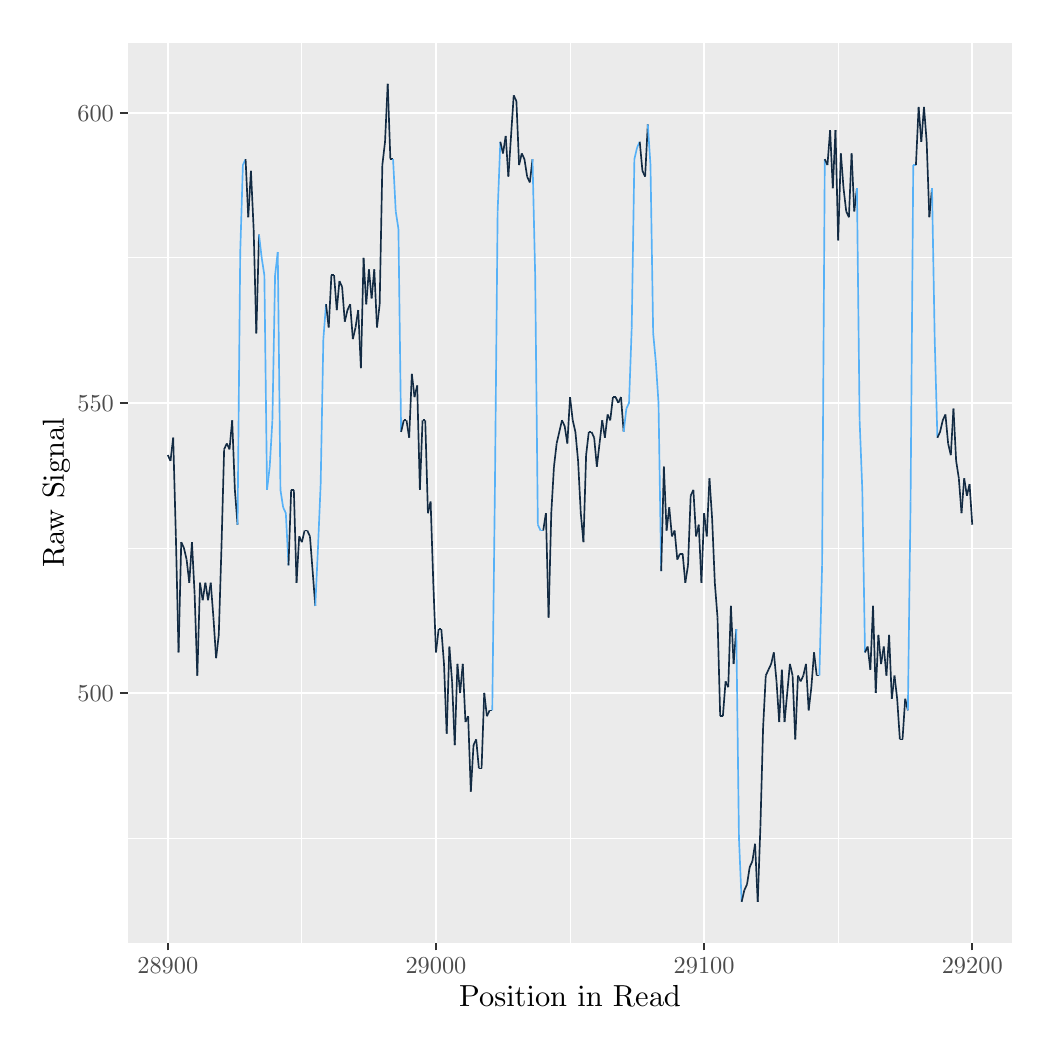
\begin{tikzpicture}[x=1pt,y=1pt]
\definecolor{fillColor}{RGB}{255,255,255}
\path[use as bounding box,fill=fillColor,fill opacity=0.00] (0,0) rectangle (361.35,361.35);
\begin{scope}
\path[clip] (  0.00,  0.00) rectangle (361.35,361.35);
\definecolor{drawColor}{RGB}{255,255,255}
\definecolor{fillColor}{RGB}{255,255,255}

\path[draw=drawColor,line width= 0.6pt,line join=round,line cap=round,fill=fillColor] (  0.00,  0.00) rectangle (361.35,361.35);
\end{scope}
\begin{scope}
\path[clip] ( 36.11, 30.69) rectangle (355.85,355.85);
\definecolor{fillColor}{gray}{0.92}

\path[fill=fillColor] ( 36.11, 30.69) rectangle (355.85,355.85);
\definecolor{drawColor}{RGB}{255,255,255}

\path[draw=drawColor,line width= 0.3pt,line join=round] ( 36.11, 68.53) --
	(355.85, 68.53);

\path[draw=drawColor,line width= 0.3pt,line join=round] ( 36.11,173.35) --
	(355.85,173.35);

\path[draw=drawColor,line width= 0.3pt,line join=round] ( 36.11,278.18) --
	(355.85,278.18);

\path[draw=drawColor,line width= 0.3pt,line join=round] ( 99.09, 30.69) --
	( 99.09,355.85);

\path[draw=drawColor,line width= 0.3pt,line join=round] (195.98, 30.69) --
	(195.98,355.85);

\path[draw=drawColor,line width= 0.3pt,line join=round] (292.87, 30.69) --
	(292.87,355.85);

\path[draw=drawColor,line width= 0.6pt,line join=round] ( 36.11,120.94) --
	(355.85,120.94);

\path[draw=drawColor,line width= 0.6pt,line join=round] ( 36.11,225.76) --
	(355.85,225.76);

\path[draw=drawColor,line width= 0.6pt,line join=round] ( 36.11,330.59) --
	(355.85,330.59);

\path[draw=drawColor,line width= 0.6pt,line join=round] ( 50.64, 30.69) --
	( 50.64,355.85);

\path[draw=drawColor,line width= 0.6pt,line join=round] (147.54, 30.69) --
	(147.54,355.85);

\path[draw=drawColor,line width= 0.6pt,line join=round] (244.43, 30.69) --
	(244.43,355.85);

\path[draw=drawColor,line width= 0.6pt,line join=round] (341.32, 30.69) --
	(341.32,355.85);
\definecolor{drawColor}{RGB}{19,43,67}

\path[draw=drawColor,line width= 0.6pt,line join=round] ( 50.64,206.90) -- ( 51.61,204.80);

\path[draw=drawColor,line width= 0.6pt,line join=round] ( 51.61,204.80) -- ( 52.58,213.18);

\path[draw=drawColor,line width= 0.6pt,line join=round] ( 52.58,213.18) -- ( 53.55,177.54);

\path[draw=drawColor,line width= 0.6pt,line join=round] ( 53.55,177.54) -- ( 54.52,135.61);

\path[draw=drawColor,line width= 0.6pt,line join=round] ( 54.52,135.61) -- ( 55.49,175.45);

\path[draw=drawColor,line width= 0.6pt,line join=round] ( 55.49,175.45) -- ( 56.46,173.35);

\path[draw=drawColor,line width= 0.6pt,line join=round] ( 56.46,173.35) -- ( 57.43,169.16);

\path[draw=drawColor,line width= 0.6pt,line join=round] ( 57.43,169.16) -- ( 58.40,160.77);

\path[draw=drawColor,line width= 0.6pt,line join=round] ( 58.40,160.77) -- ( 59.36,175.45);

\path[draw=drawColor,line width= 0.6pt,line join=round] ( 59.36,175.45) -- ( 60.33,156.58);

\path[draw=drawColor,line width= 0.6pt,line join=round] ( 60.33,156.58) -- ( 61.30,127.23);

\path[draw=drawColor,line width= 0.6pt,line join=round] ( 61.30,127.23) -- ( 62.27,160.77);

\path[draw=drawColor,line width= 0.6pt,line join=round] ( 62.27,160.77) -- ( 63.24,154.48);

\path[draw=drawColor,line width= 0.6pt,line join=round] ( 63.24,154.48) -- ( 64.21,160.77);

\path[draw=drawColor,line width= 0.6pt,line join=round] ( 64.21,160.77) -- ( 65.18,154.48);

\path[draw=drawColor,line width= 0.6pt,line join=round] ( 65.18,154.48) -- ( 66.15,160.77);

\path[draw=drawColor,line width= 0.6pt,line join=round] ( 66.15,160.77) -- ( 67.12,148.19);

\path[draw=drawColor,line width= 0.6pt,line join=round] ( 67.12,148.19) -- ( 68.09,133.52);

\path[draw=drawColor,line width= 0.6pt,line join=round] ( 68.09,133.52) -- ( 69.05,141.90);

\path[draw=drawColor,line width= 0.6pt,line join=round] ( 69.05,141.90) -- ( 70.02,173.35);

\path[draw=drawColor,line width= 0.6pt,line join=round] ( 70.02,173.35) -- ( 70.99,208.99);

\path[draw=drawColor,line width= 0.6pt,line join=round] ( 70.99,208.99) -- ( 71.96,211.09);

\path[draw=drawColor,line width= 0.6pt,line join=round] ( 71.96,211.09) -- ( 72.93,208.99);

\path[draw=drawColor,line width= 0.6pt,line join=round] ( 72.93,208.99) -- ( 73.90,219.47);

\path[draw=drawColor,line width= 0.6pt,line join=round] ( 73.90,219.47) -- ( 74.87,194.32);

\path[draw=drawColor,line width= 0.6pt,line join=round] ( 74.87,194.32) -- ( 75.84,181.74);
\definecolor{drawColor}{RGB}{86,177,247}

\path[draw=drawColor,line width= 0.6pt,line join=round] ( 75.84,181.74) -- ( 76.81,280.27);

\path[draw=drawColor,line width= 0.6pt,line join=round] ( 76.81,280.27) -- ( 77.77,311.72);

\path[draw=drawColor,line width= 0.6pt,line join=round] ( 77.77,311.72) -- ( 78.74,313.82);
\definecolor{drawColor}{RGB}{19,43,67}

\path[draw=drawColor,line width= 0.6pt,line join=round] ( 78.74,313.82) -- ( 79.71,292.85);

\path[draw=drawColor,line width= 0.6pt,line join=round] ( 79.71,292.85) -- ( 80.68,309.62);

\path[draw=drawColor,line width= 0.6pt,line join=round] ( 80.68,309.62) -- ( 81.65,288.66);

\path[draw=drawColor,line width= 0.6pt,line join=round] ( 81.65,288.66) -- ( 82.62,250.92);

\path[draw=drawColor,line width= 0.6pt,line join=round] ( 82.62,250.92) -- ( 83.59,286.56);
\definecolor{drawColor}{RGB}{86,177,247}

\path[draw=drawColor,line width= 0.6pt,line join=round] ( 83.59,286.56) -- ( 84.56,278.18);

\path[draw=drawColor,line width= 0.6pt,line join=round] ( 84.56,278.18) -- ( 85.53,271.89);

\path[draw=drawColor,line width= 0.6pt,line join=round] ( 85.53,271.89) -- ( 86.49,194.32);

\path[draw=drawColor,line width= 0.6pt,line join=round] ( 86.49,194.32) -- ( 87.46,202.70);

\path[draw=drawColor,line width= 0.6pt,line join=round] ( 87.46,202.70) -- ( 88.43,219.47);

\path[draw=drawColor,line width= 0.6pt,line join=round] ( 88.43,219.47) -- ( 89.40,271.89);

\path[draw=drawColor,line width= 0.6pt,line join=round] ( 89.40,271.89) -- ( 90.37,280.27);

\path[draw=drawColor,line width= 0.6pt,line join=round] ( 90.37,280.27) -- ( 91.34,194.32);

\path[draw=drawColor,line width= 0.6pt,line join=round] ( 91.34,194.32) -- ( 92.31,188.03);

\path[draw=drawColor,line width= 0.6pt,line join=round] ( 92.31,188.03) -- ( 93.28,185.93);

\path[draw=drawColor,line width= 0.6pt,line join=round] ( 93.28,185.93) -- ( 94.25,167.06);
\definecolor{drawColor}{RGB}{19,43,67}

\path[draw=drawColor,line width= 0.6pt,line join=round] ( 94.25,167.06) -- ( 95.21,194.32);

\path[draw=drawColor,line width= 0.6pt,line join=round] ( 95.21,194.32) -- ( 96.18,194.32);

\path[draw=drawColor,line width= 0.6pt,line join=round] ( 96.18,194.32) -- ( 97.15,160.77);

\path[draw=drawColor,line width= 0.6pt,line join=round] ( 97.15,160.77) -- ( 98.12,177.54);

\path[draw=drawColor,line width= 0.6pt,line join=round] ( 98.12,177.54) -- ( 99.09,175.45);

\path[draw=drawColor,line width= 0.6pt,line join=round] ( 99.09,175.45) -- (100.06,179.64);

\path[draw=drawColor,line width= 0.6pt,line join=round] (100.06,179.64) -- (101.03,179.64);

\path[draw=drawColor,line width= 0.6pt,line join=round] (101.03,179.64) -- (102.00,177.54);

\path[draw=drawColor,line width= 0.6pt,line join=round] (102.00,177.54) -- (102.97,164.97);

\path[draw=drawColor,line width= 0.6pt,line join=round] (102.97,164.97) -- (103.93,152.39);
\definecolor{drawColor}{RGB}{86,177,247}

\path[draw=drawColor,line width= 0.6pt,line join=round] (103.93,152.39) -- (104.90,173.35);

\path[draw=drawColor,line width= 0.6pt,line join=round] (104.90,173.35) -- (105.87,196.41);

\path[draw=drawColor,line width= 0.6pt,line join=round] (105.87,196.41) -- (106.84,248.82);

\path[draw=drawColor,line width= 0.6pt,line join=round] (106.84,248.82) -- (107.81,261.40);
\definecolor{drawColor}{RGB}{19,43,67}

\path[draw=drawColor,line width= 0.6pt,line join=round] (107.81,261.40) -- (108.78,253.02);

\path[draw=drawColor,line width= 0.6pt,line join=round] (108.78,253.02) -- (109.75,271.89);

\path[draw=drawColor,line width= 0.6pt,line join=round] (109.75,271.89) -- (110.72,271.89);

\path[draw=drawColor,line width= 0.6pt,line join=round] (110.72,271.89) -- (111.69,259.31);

\path[draw=drawColor,line width= 0.6pt,line join=round] (111.69,259.31) -- (112.65,269.79);

\path[draw=drawColor,line width= 0.6pt,line join=round] (112.65,269.79) -- (113.62,267.69);

\path[draw=drawColor,line width= 0.6pt,line join=round] (113.62,267.69) -- (114.59,255.11);

\path[draw=drawColor,line width= 0.6pt,line join=round] (114.59,255.11) -- (115.56,259.31);

\path[draw=drawColor,line width= 0.6pt,line join=round] (115.56,259.31) -- (116.53,261.40);

\path[draw=drawColor,line width= 0.6pt,line join=round] (116.53,261.40) -- (117.50,248.82);

\path[draw=drawColor,line width= 0.6pt,line join=round] (117.50,248.82) -- (118.47,253.02);

\path[draw=drawColor,line width= 0.6pt,line join=round] (118.47,253.02) -- (119.44,259.31);

\path[draw=drawColor,line width= 0.6pt,line join=round] (119.44,259.31) -- (120.41,238.34);

\path[draw=drawColor,line width= 0.6pt,line join=round] (120.41,238.34) -- (121.37,278.18);

\path[draw=drawColor,line width= 0.6pt,line join=round] (121.37,278.18) -- (122.34,261.40);

\path[draw=drawColor,line width= 0.6pt,line join=round] (122.34,261.40) -- (123.31,273.98);

\path[draw=drawColor,line width= 0.6pt,line join=round] (123.31,273.98) -- (124.28,263.50);

\path[draw=drawColor,line width= 0.6pt,line join=round] (124.28,263.50) -- (125.25,273.98);

\path[draw=drawColor,line width= 0.6pt,line join=round] (125.25,273.98) -- (126.22,253.02);

\path[draw=drawColor,line width= 0.6pt,line join=round] (126.22,253.02) -- (127.19,261.40);

\path[draw=drawColor,line width= 0.6pt,line join=round] (127.19,261.40) -- (128.16,311.72);

\path[draw=drawColor,line width= 0.6pt,line join=round] (128.16,311.72) -- (129.13,320.11);

\path[draw=drawColor,line width= 0.6pt,line join=round] (129.13,320.11) -- (130.10,341.07);

\path[draw=drawColor,line width= 0.6pt,line join=round] (130.10,341.07) -- (131.06,313.82);

\path[draw=drawColor,line width= 0.6pt,line join=round] (131.06,313.82) -- (132.03,313.82);
\definecolor{drawColor}{RGB}{86,177,247}

\path[draw=drawColor,line width= 0.6pt,line join=round] (132.03,313.82) -- (133.00,294.95);

\path[draw=drawColor,line width= 0.6pt,line join=round] (133.00,294.95) -- (133.97,288.66);

\path[draw=drawColor,line width= 0.6pt,line join=round] (133.97,288.66) -- (134.94,215.28);
\definecolor{drawColor}{RGB}{19,43,67}

\path[draw=drawColor,line width= 0.6pt,line join=round] (134.94,215.28) -- (135.91,219.47);

\path[draw=drawColor,line width= 0.6pt,line join=round] (135.91,219.47) -- (136.88,219.47);

\path[draw=drawColor,line width= 0.6pt,line join=round] (136.88,219.47) -- (137.85,213.18);

\path[draw=drawColor,line width= 0.6pt,line join=round] (137.85,213.18) -- (138.82,236.25);

\path[draw=drawColor,line width= 0.6pt,line join=round] (138.82,236.25) -- (139.78,227.86);

\path[draw=drawColor,line width= 0.6pt,line join=round] (139.78,227.86) -- (140.75,232.05);

\path[draw=drawColor,line width= 0.6pt,line join=round] (140.75,232.05) -- (141.72,194.32);

\path[draw=drawColor,line width= 0.6pt,line join=round] (141.72,194.32) -- (142.69,219.47);

\path[draw=drawColor,line width= 0.6pt,line join=round] (142.69,219.47) -- (143.66,219.47);

\path[draw=drawColor,line width= 0.6pt,line join=round] (143.66,219.47) -- (144.63,185.93);

\path[draw=drawColor,line width= 0.6pt,line join=round] (144.63,185.93) -- (145.60,190.12);

\path[draw=drawColor,line width= 0.6pt,line join=round] (145.60,190.12) -- (146.57,160.77);

\path[draw=drawColor,line width= 0.6pt,line join=round] (146.57,160.77) -- (147.54,135.61);

\path[draw=drawColor,line width= 0.6pt,line join=round] (147.54,135.61) -- (148.50,144.00);

\path[draw=drawColor,line width= 0.6pt,line join=round] (148.50,144.00) -- (149.47,144.00);

\path[draw=drawColor,line width= 0.6pt,line join=round] (149.47,144.00) -- (150.44,131.42);

\path[draw=drawColor,line width= 0.6pt,line join=round] (150.44,131.42) -- (151.41,106.26);

\path[draw=drawColor,line width= 0.6pt,line join=round] (151.41,106.26) -- (152.38,137.71);

\path[draw=drawColor,line width= 0.6pt,line join=round] (152.38,137.71) -- (153.35,125.13);

\path[draw=drawColor,line width= 0.6pt,line join=round] (153.35,125.13) -- (154.32,102.07);

\path[draw=drawColor,line width= 0.6pt,line join=round] (154.32,102.07) -- (155.29,131.42);

\path[draw=drawColor,line width= 0.6pt,line join=round] (155.29,131.42) -- (156.26,120.94);

\path[draw=drawColor,line width= 0.6pt,line join=round] (156.26,120.94) -- (157.22,131.42);

\path[draw=drawColor,line width= 0.6pt,line join=round] (157.22,131.42) -- (158.19,110.46);

\path[draw=drawColor,line width= 0.6pt,line join=round] (158.19,110.46) -- (159.16,112.55);

\path[draw=drawColor,line width= 0.6pt,line join=round] (159.16,112.55) -- (160.13, 85.30);

\path[draw=drawColor,line width= 0.6pt,line join=round] (160.13, 85.30) -- (161.10,102.07);

\path[draw=drawColor,line width= 0.6pt,line join=round] (161.10,102.07) -- (162.07,104.17);

\path[draw=drawColor,line width= 0.6pt,line join=round] (162.07,104.17) -- (163.04, 93.69);

\path[draw=drawColor,line width= 0.6pt,line join=round] (163.04, 93.69) -- (164.01, 93.69);

\path[draw=drawColor,line width= 0.6pt,line join=round] (164.01, 93.69) -- (164.98,120.94);

\path[draw=drawColor,line width= 0.6pt,line join=round] (164.98,120.94) -- (165.94,112.55);

\path[draw=drawColor,line width= 0.6pt,line join=round] (165.94,112.55) -- (166.91,114.65);

\path[draw=drawColor,line width= 0.6pt,line join=round] (166.91,114.65) -- (167.88,114.65);
\definecolor{drawColor}{RGB}{86,177,247}

\path[draw=drawColor,line width= 0.6pt,line join=round] (167.88,114.65) -- (168.85,196.41);

\path[draw=drawColor,line width= 0.6pt,line join=round] (168.85,196.41) -- (169.82,294.95);

\path[draw=drawColor,line width= 0.6pt,line join=round] (169.82,294.95) -- (170.79,320.11);
\definecolor{drawColor}{RGB}{19,43,67}

\path[draw=drawColor,line width= 0.6pt,line join=round] (170.79,320.11) -- (171.76,315.91);

\path[draw=drawColor,line width= 0.6pt,line join=round] (171.76,315.91) -- (172.73,322.20);

\path[draw=drawColor,line width= 0.6pt,line join=round] (172.73,322.20) -- (173.70,307.53);

\path[draw=drawColor,line width= 0.6pt,line join=round] (173.70,307.53) -- (174.66,322.20);

\path[draw=drawColor,line width= 0.6pt,line join=round] (174.66,322.20) -- (175.63,336.88);

\path[draw=drawColor,line width= 0.6pt,line join=round] (175.63,336.88) -- (176.60,334.78);

\path[draw=drawColor,line width= 0.6pt,line join=round] (176.60,334.78) -- (177.57,311.72);

\path[draw=drawColor,line width= 0.6pt,line join=round] (177.57,311.72) -- (178.54,315.91);

\path[draw=drawColor,line width= 0.6pt,line join=round] (178.54,315.91) -- (179.51,313.82);

\path[draw=drawColor,line width= 0.6pt,line join=round] (179.51,313.82) -- (180.48,307.53);

\path[draw=drawColor,line width= 0.6pt,line join=round] (180.48,307.53) -- (181.45,305.43);

\path[draw=drawColor,line width= 0.6pt,line join=round] (181.45,305.43) -- (182.42,313.82);
\definecolor{drawColor}{RGB}{86,177,247}

\path[draw=drawColor,line width= 0.6pt,line join=round] (182.42,313.82) -- (183.38,271.89);

\path[draw=drawColor,line width= 0.6pt,line join=round] (183.38,271.89) -- (184.35,181.74);

\path[draw=drawColor,line width= 0.6pt,line join=round] (184.35,181.74) -- (185.32,179.64);

\path[draw=drawColor,line width= 0.6pt,line join=round] (185.32,179.64) -- (186.29,179.64);
\definecolor{drawColor}{RGB}{19,43,67}

\path[draw=drawColor,line width= 0.6pt,line join=round] (186.29,179.64) -- (187.26,185.93);

\path[draw=drawColor,line width= 0.6pt,line join=round] (187.26,185.93) -- (188.23,148.19);

\path[draw=drawColor,line width= 0.6pt,line join=round] (188.23,148.19) -- (189.20,185.93);

\path[draw=drawColor,line width= 0.6pt,line join=round] (189.20,185.93) -- (190.17,202.70);

\path[draw=drawColor,line width= 0.6pt,line join=round] (190.17,202.70) -- (191.14,211.09);

\path[draw=drawColor,line width= 0.6pt,line join=round] (191.14,211.09) -- (192.10,215.28);

\path[draw=drawColor,line width= 0.6pt,line join=round] (192.10,215.28) -- (193.07,219.47);

\path[draw=drawColor,line width= 0.6pt,line join=round] (193.07,219.47) -- (194.04,217.38);

\path[draw=drawColor,line width= 0.6pt,line join=round] (194.04,217.38) -- (195.01,211.09);

\path[draw=drawColor,line width= 0.6pt,line join=round] (195.01,211.09) -- (195.98,227.86);

\path[draw=drawColor,line width= 0.6pt,line join=round] (195.98,227.86) -- (196.95,219.47);

\path[draw=drawColor,line width= 0.6pt,line join=round] (196.95,219.47) -- (197.92,215.28);

\path[draw=drawColor,line width= 0.6pt,line join=round] (197.92,215.28) -- (198.89,204.80);

\path[draw=drawColor,line width= 0.6pt,line join=round] (198.89,204.80) -- (199.86,185.93);

\path[draw=drawColor,line width= 0.6pt,line join=round] (199.86,185.93) -- (200.83,175.45);

\path[draw=drawColor,line width= 0.6pt,line join=round] (200.83,175.45) -- (201.79,206.90);

\path[draw=drawColor,line width= 0.6pt,line join=round] (201.79,206.90) -- (202.76,215.28);

\path[draw=drawColor,line width= 0.6pt,line join=round] (202.76,215.28) -- (203.73,215.28);

\path[draw=drawColor,line width= 0.6pt,line join=round] (203.73,215.28) -- (204.70,213.18);

\path[draw=drawColor,line width= 0.6pt,line join=round] (204.70,213.18) -- (205.67,202.70);

\path[draw=drawColor,line width= 0.6pt,line join=round] (205.67,202.70) -- (206.64,211.09);

\path[draw=drawColor,line width= 0.6pt,line join=round] (206.64,211.09) -- (207.61,219.47);

\path[draw=drawColor,line width= 0.6pt,line join=round] (207.61,219.47) -- (208.58,213.18);

\path[draw=drawColor,line width= 0.6pt,line join=round] (208.58,213.18) -- (209.55,221.57);

\path[draw=drawColor,line width= 0.6pt,line join=round] (209.55,221.57) -- (210.51,219.47);

\path[draw=drawColor,line width= 0.6pt,line join=round] (210.51,219.47) -- (211.48,227.86);

\path[draw=drawColor,line width= 0.6pt,line join=round] (211.48,227.86) -- (212.45,227.86);

\path[draw=drawColor,line width= 0.6pt,line join=round] (212.45,227.86) -- (213.42,225.76);

\path[draw=drawColor,line width= 0.6pt,line join=round] (213.42,225.76) -- (214.39,227.86);

\path[draw=drawColor,line width= 0.6pt,line join=round] (214.39,227.86) -- (215.36,215.28);
\definecolor{drawColor}{RGB}{86,177,247}

\path[draw=drawColor,line width= 0.6pt,line join=round] (215.36,215.28) -- (216.33,223.67);

\path[draw=drawColor,line width= 0.6pt,line join=round] (216.33,223.67) -- (217.30,225.76);

\path[draw=drawColor,line width= 0.6pt,line join=round] (217.30,225.76) -- (218.27,253.02);

\path[draw=drawColor,line width= 0.6pt,line join=round] (218.27,253.02) -- (219.23,313.82);

\path[draw=drawColor,line width= 0.6pt,line join=round] (219.23,313.82) -- (220.20,318.01);

\path[draw=drawColor,line width= 0.6pt,line join=round] (220.20,318.01) -- (221.17,320.11);
\definecolor{drawColor}{RGB}{19,43,67}

\path[draw=drawColor,line width= 0.6pt,line join=round] (221.17,320.11) -- (222.14,309.62);

\path[draw=drawColor,line width= 0.6pt,line join=round] (222.14,309.62) -- (223.11,307.53);

\path[draw=drawColor,line width= 0.6pt,line join=round] (223.11,307.53) -- (224.08,326.39);
\definecolor{drawColor}{RGB}{86,177,247}

\path[draw=drawColor,line width= 0.6pt,line join=round] (224.08,326.39) -- (225.05,311.72);

\path[draw=drawColor,line width= 0.6pt,line join=round] (225.05,311.72) -- (226.02,250.92);

\path[draw=drawColor,line width= 0.6pt,line join=round] (226.02,250.92) -- (226.99,240.44);

\path[draw=drawColor,line width= 0.6pt,line join=round] (226.99,240.44) -- (227.95,225.76);

\path[draw=drawColor,line width= 0.6pt,line join=round] (227.95,225.76) -- (228.92,164.97);
\definecolor{drawColor}{RGB}{19,43,67}

\path[draw=drawColor,line width= 0.6pt,line join=round] (228.92,164.97) -- (229.89,202.70);

\path[draw=drawColor,line width= 0.6pt,line join=round] (229.89,202.70) -- (230.86,179.64);

\path[draw=drawColor,line width= 0.6pt,line join=round] (230.86,179.64) -- (231.83,188.03);

\path[draw=drawColor,line width= 0.6pt,line join=round] (231.83,188.03) -- (232.80,177.54);

\path[draw=drawColor,line width= 0.6pt,line join=round] (232.80,177.54) -- (233.77,179.64);

\path[draw=drawColor,line width= 0.6pt,line join=round] (233.77,179.64) -- (234.74,169.16);

\path[draw=drawColor,line width= 0.6pt,line join=round] (234.74,169.16) -- (235.71,171.25);

\path[draw=drawColor,line width= 0.6pt,line join=round] (235.71,171.25) -- (236.67,171.25);

\path[draw=drawColor,line width= 0.6pt,line join=round] (236.67,171.25) -- (237.64,160.77);

\path[draw=drawColor,line width= 0.6pt,line join=round] (237.64,160.77) -- (238.61,167.06);

\path[draw=drawColor,line width= 0.6pt,line join=round] (238.61,167.06) -- (239.58,192.22);

\path[draw=drawColor,line width= 0.6pt,line join=round] (239.58,192.22) -- (240.55,194.32);

\path[draw=drawColor,line width= 0.6pt,line join=round] (240.55,194.32) -- (241.52,177.54);

\path[draw=drawColor,line width= 0.6pt,line join=round] (241.52,177.54) -- (242.49,181.74);

\path[draw=drawColor,line width= 0.6pt,line join=round] (242.49,181.74) -- (243.46,160.77);

\path[draw=drawColor,line width= 0.6pt,line join=round] (243.46,160.77) -- (244.43,185.93);

\path[draw=drawColor,line width= 0.6pt,line join=round] (244.43,185.93) -- (245.39,177.54);

\path[draw=drawColor,line width= 0.6pt,line join=round] (245.39,177.54) -- (246.36,198.51);

\path[draw=drawColor,line width= 0.6pt,line join=round] (246.36,198.51) -- (247.33,183.83);

\path[draw=drawColor,line width= 0.6pt,line join=round] (247.33,183.83) -- (248.30,160.77);

\path[draw=drawColor,line width= 0.6pt,line join=round] (248.30,160.77) -- (249.27,148.19);

\path[draw=drawColor,line width= 0.6pt,line join=round] (249.27,148.19) -- (250.24,112.55);

\path[draw=drawColor,line width= 0.6pt,line join=round] (250.24,112.55) -- (251.21,112.55);

\path[draw=drawColor,line width= 0.6pt,line join=round] (251.21,112.55) -- (252.18,125.13);

\path[draw=drawColor,line width= 0.6pt,line join=round] (252.18,125.13) -- (253.15,123.04);

\path[draw=drawColor,line width= 0.6pt,line join=round] (253.15,123.04) -- (254.11,152.39);

\path[draw=drawColor,line width= 0.6pt,line join=round] (254.11,152.39) -- (255.08,131.42);

\path[draw=drawColor,line width= 0.6pt,line join=round] (255.08,131.42) -- (256.05,144.00);
\definecolor{drawColor}{RGB}{86,177,247}

\path[draw=drawColor,line width= 0.6pt,line join=round] (256.05,144.00) -- (257.02, 68.53);

\path[draw=drawColor,line width= 0.6pt,line join=round] (257.02, 68.53) -- (257.99, 45.47);
\definecolor{drawColor}{RGB}{19,43,67}

\path[draw=drawColor,line width= 0.6pt,line join=round] (257.99, 45.47) -- (258.96, 49.66);

\path[draw=drawColor,line width= 0.6pt,line join=round] (258.96, 49.66) -- (259.93, 51.76);

\path[draw=drawColor,line width= 0.6pt,line join=round] (259.93, 51.76) -- (260.90, 58.04);

\path[draw=drawColor,line width= 0.6pt,line join=round] (260.90, 58.04) -- (261.87, 60.14);

\path[draw=drawColor,line width= 0.6pt,line join=round] (261.87, 60.14) -- (262.84, 66.43);

\path[draw=drawColor,line width= 0.6pt,line join=round] (262.84, 66.43) -- (263.80, 45.47);

\path[draw=drawColor,line width= 0.6pt,line join=round] (263.80, 45.47) -- (264.77, 72.72);

\path[draw=drawColor,line width= 0.6pt,line join=round] (264.77, 72.72) -- (265.74,108.36);

\path[draw=drawColor,line width= 0.6pt,line join=round] (265.74,108.36) -- (266.71,127.23);

\path[draw=drawColor,line width= 0.6pt,line join=round] (266.71,127.23) -- (267.68,129.33);

\path[draw=drawColor,line width= 0.6pt,line join=round] (267.68,129.33) -- (268.65,131.42);

\path[draw=drawColor,line width= 0.6pt,line join=round] (268.65,131.42) -- (269.62,135.61);

\path[draw=drawColor,line width= 0.6pt,line join=round] (269.62,135.61) -- (270.59,125.13);

\path[draw=drawColor,line width= 0.6pt,line join=round] (270.59,125.13) -- (271.56,110.46);

\path[draw=drawColor,line width= 0.6pt,line join=round] (271.56,110.46) -- (272.52,129.33);

\path[draw=drawColor,line width= 0.6pt,line join=round] (272.52,129.33) -- (273.49,110.46);

\path[draw=drawColor,line width= 0.6pt,line join=round] (273.49,110.46) -- (274.46,120.94);

\path[draw=drawColor,line width= 0.6pt,line join=round] (274.46,120.94) -- (275.43,131.42);

\path[draw=drawColor,line width= 0.6pt,line join=round] (275.43,131.42) -- (276.40,127.23);

\path[draw=drawColor,line width= 0.6pt,line join=round] (276.40,127.23) -- (277.37,104.17);

\path[draw=drawColor,line width= 0.6pt,line join=round] (277.37,104.17) -- (278.34,127.23);

\path[draw=drawColor,line width= 0.6pt,line join=round] (278.34,127.23) -- (279.31,125.13);

\path[draw=drawColor,line width= 0.6pt,line join=round] (279.31,125.13) -- (280.28,127.23);

\path[draw=drawColor,line width= 0.6pt,line join=round] (280.28,127.23) -- (281.24,131.42);

\path[draw=drawColor,line width= 0.6pt,line join=round] (281.24,131.42) -- (282.21,114.65);

\path[draw=drawColor,line width= 0.6pt,line join=round] (282.21,114.65) -- (283.18,123.04);

\path[draw=drawColor,line width= 0.6pt,line join=round] (283.18,123.04) -- (284.15,135.61);

\path[draw=drawColor,line width= 0.6pt,line join=round] (284.15,135.61) -- (285.12,127.23);

\path[draw=drawColor,line width= 0.6pt,line join=round] (285.12,127.23) -- (286.09,127.23);
\definecolor{drawColor}{RGB}{86,177,247}

\path[draw=drawColor,line width= 0.6pt,line join=round] (286.09,127.23) -- (287.06,167.06);

\path[draw=drawColor,line width= 0.6pt,line join=round] (287.06,167.06) -- (288.03,313.82);
\definecolor{drawColor}{RGB}{19,43,67}

\path[draw=drawColor,line width= 0.6pt,line join=round] (288.03,313.82) -- (289.00,311.72);

\path[draw=drawColor,line width= 0.6pt,line join=round] (289.00,311.72) -- (289.96,324.30);

\path[draw=drawColor,line width= 0.6pt,line join=round] (289.96,324.30) -- (290.93,303.33);

\path[draw=drawColor,line width= 0.6pt,line join=round] (290.93,303.33) -- (291.90,324.30);

\path[draw=drawColor,line width= 0.6pt,line join=round] (291.90,324.30) -- (292.87,284.46);

\path[draw=drawColor,line width= 0.6pt,line join=round] (292.87,284.46) -- (293.84,315.91);

\path[draw=drawColor,line width= 0.6pt,line join=round] (293.84,315.91) -- (294.81,303.33);

\path[draw=drawColor,line width= 0.6pt,line join=round] (294.81,303.33) -- (295.78,294.95);

\path[draw=drawColor,line width= 0.6pt,line join=round] (295.78,294.95) -- (296.75,292.85);

\path[draw=drawColor,line width= 0.6pt,line join=round] (296.75,292.85) -- (297.72,315.91);

\path[draw=drawColor,line width= 0.6pt,line join=round] (297.72,315.91) -- (298.68,294.95);

\path[draw=drawColor,line width= 0.6pt,line join=round] (298.68,294.95) -- (299.65,303.33);
\definecolor{drawColor}{RGB}{86,177,247}

\path[draw=drawColor,line width= 0.6pt,line join=round] (299.65,303.33) -- (300.62,219.47);

\path[draw=drawColor,line width= 0.6pt,line join=round] (300.62,219.47) -- (301.59,194.32);

\path[draw=drawColor,line width= 0.6pt,line join=round] (301.59,194.32) -- (302.56,135.61);
\definecolor{drawColor}{RGB}{19,43,67}

\path[draw=drawColor,line width= 0.6pt,line join=round] (302.56,135.61) -- (303.53,137.71);

\path[draw=drawColor,line width= 0.6pt,line join=round] (303.53,137.71) -- (304.50,129.33);

\path[draw=drawColor,line width= 0.6pt,line join=round] (304.50,129.33) -- (305.47,152.39);

\path[draw=drawColor,line width= 0.6pt,line join=round] (305.47,152.39) -- (306.44,120.94);

\path[draw=drawColor,line width= 0.6pt,line join=round] (306.44,120.94) -- (307.40,141.90);

\path[draw=drawColor,line width= 0.6pt,line join=round] (307.40,141.90) -- (308.37,131.42);

\path[draw=drawColor,line width= 0.6pt,line join=round] (308.37,131.42) -- (309.34,137.71);

\path[draw=drawColor,line width= 0.6pt,line join=round] (309.34,137.71) -- (310.31,127.23);

\path[draw=drawColor,line width= 0.6pt,line join=round] (310.31,127.23) -- (311.28,141.90);

\path[draw=drawColor,line width= 0.6pt,line join=round] (311.28,141.90) -- (312.25,118.84);

\path[draw=drawColor,line width= 0.6pt,line join=round] (312.25,118.84) -- (313.22,127.23);

\path[draw=drawColor,line width= 0.6pt,line join=round] (313.22,127.23) -- (314.19,118.84);

\path[draw=drawColor,line width= 0.6pt,line join=round] (314.19,118.84) -- (315.16,104.17);

\path[draw=drawColor,line width= 0.6pt,line join=round] (315.16,104.17) -- (316.12,104.17);

\path[draw=drawColor,line width= 0.6pt,line join=round] (316.12,104.17) -- (317.09,118.84);

\path[draw=drawColor,line width= 0.6pt,line join=round] (317.09,118.84) -- (318.06,114.65);
\definecolor{drawColor}{RGB}{86,177,247}

\path[draw=drawColor,line width= 0.6pt,line join=round] (318.06,114.65) -- (319.03,190.12);

\path[draw=drawColor,line width= 0.6pt,line join=round] (319.03,190.12) -- (320.00,311.72);

\path[draw=drawColor,line width= 0.6pt,line join=round] (320.00,311.72) -- (320.97,311.72);
\definecolor{drawColor}{RGB}{19,43,67}

\path[draw=drawColor,line width= 0.6pt,line join=round] (320.97,311.72) -- (321.94,332.68);

\path[draw=drawColor,line width= 0.6pt,line join=round] (321.94,332.68) -- (322.91,320.11);

\path[draw=drawColor,line width= 0.6pt,line join=round] (322.91,320.11) -- (323.88,332.68);

\path[draw=drawColor,line width= 0.6pt,line join=round] (323.88,332.68) -- (324.85,320.11);

\path[draw=drawColor,line width= 0.6pt,line join=round] (324.85,320.11) -- (325.81,292.85);

\path[draw=drawColor,line width= 0.6pt,line join=round] (325.81,292.85) -- (326.78,303.33);
\definecolor{drawColor}{RGB}{86,177,247}

\path[draw=drawColor,line width= 0.6pt,line join=round] (326.78,303.33) -- (327.75,248.82);

\path[draw=drawColor,line width= 0.6pt,line join=round] (327.75,248.82) -- (328.72,213.18);
\definecolor{drawColor}{RGB}{19,43,67}

\path[draw=drawColor,line width= 0.6pt,line join=round] (328.72,213.18) -- (329.69,215.28);

\path[draw=drawColor,line width= 0.6pt,line join=round] (329.69,215.28) -- (330.66,219.47);

\path[draw=drawColor,line width= 0.6pt,line join=round] (330.66,219.47) -- (331.63,221.57);

\path[draw=drawColor,line width= 0.6pt,line join=round] (331.63,221.57) -- (332.60,211.09);

\path[draw=drawColor,line width= 0.6pt,line join=round] (332.60,211.09) -- (333.57,206.90);

\path[draw=drawColor,line width= 0.6pt,line join=round] (333.57,206.90) -- (334.53,223.67);

\path[draw=drawColor,line width= 0.6pt,line join=round] (334.53,223.67) -- (335.50,204.80);

\path[draw=drawColor,line width= 0.6pt,line join=round] (335.50,204.80) -- (336.47,198.51);

\path[draw=drawColor,line width= 0.6pt,line join=round] (336.47,198.51) -- (337.44,185.93);

\path[draw=drawColor,line width= 0.6pt,line join=round] (337.44,185.93) -- (338.41,198.51);

\path[draw=drawColor,line width= 0.6pt,line join=round] (338.41,198.51) -- (339.38,192.22);

\path[draw=drawColor,line width= 0.6pt,line join=round] (339.38,192.22) -- (340.35,196.41);

\path[draw=drawColor,line width= 0.6pt,line join=round] (340.35,196.41) -- (341.32,181.74);
\end{scope}
\begin{scope}
\path[clip] (  0.00,  0.00) rectangle (361.35,361.35);
\definecolor{drawColor}{gray}{0.30}

\node[text=drawColor,anchor=base east,inner sep=0pt, outer sep=0pt, scale=  0.88] at ( 31.16,117.91) {500};

\node[text=drawColor,anchor=base east,inner sep=0pt, outer sep=0pt, scale=  0.88] at ( 31.16,222.73) {550};

\node[text=drawColor,anchor=base east,inner sep=0pt, outer sep=0pt, scale=  0.88] at ( 31.16,327.56) {600};
\end{scope}
\begin{scope}
\path[clip] (  0.00,  0.00) rectangle (361.35,361.35);
\definecolor{drawColor}{gray}{0.20}

\path[draw=drawColor,line width= 0.6pt,line join=round] ( 33.36,120.94) --
	( 36.11,120.94);

\path[draw=drawColor,line width= 0.6pt,line join=round] ( 33.36,225.76) --
	( 36.11,225.76);

\path[draw=drawColor,line width= 0.6pt,line join=round] ( 33.36,330.59) --
	( 36.11,330.59);
\end{scope}
\begin{scope}
\path[clip] (  0.00,  0.00) rectangle (361.35,361.35);
\definecolor{drawColor}{gray}{0.20}

\path[draw=drawColor,line width= 0.6pt,line join=round] ( 50.64, 27.94) --
	( 50.64, 30.69);

\path[draw=drawColor,line width= 0.6pt,line join=round] (147.54, 27.94) --
	(147.54, 30.69);

\path[draw=drawColor,line width= 0.6pt,line join=round] (244.43, 27.94) --
	(244.43, 30.69);

\path[draw=drawColor,line width= 0.6pt,line join=round] (341.32, 27.94) --
	(341.32, 30.69);
\end{scope}
\begin{scope}
\path[clip] (  0.00,  0.00) rectangle (361.35,361.35);
\definecolor{drawColor}{gray}{0.30}

\node[text=drawColor,anchor=base,inner sep=0pt, outer sep=0pt, scale=  0.88] at ( 50.64, 19.68) {28900};

\node[text=drawColor,anchor=base,inner sep=0pt, outer sep=0pt, scale=  0.88] at (147.54, 19.68) {29000};

\node[text=drawColor,anchor=base,inner sep=0pt, outer sep=0pt, scale=  0.88] at (244.43, 19.68) {29100};

\node[text=drawColor,anchor=base,inner sep=0pt, outer sep=0pt, scale=  0.88] at (341.32, 19.68) {29200};
\end{scope}
\begin{scope}
\path[clip] (  0.00,  0.00) rectangle (361.35,361.35);
\definecolor{drawColor}{RGB}{0,0,0}

\node[text=drawColor,anchor=base,inner sep=0pt, outer sep=0pt, scale=  1.10] at (195.98,  7.64) {Position in Read};
\end{scope}
\begin{scope}
\path[clip] (  0.00,  0.00) rectangle (361.35,361.35);
\definecolor{drawColor}{RGB}{0,0,0}

\node[text=drawColor,rotate= 90.00,anchor=base,inner sep=0pt, outer sep=0pt, scale=  1.10] at ( 13.08,193.27) {Raw Signal};
\end{scope}
\end{tikzpicture}

\caption{\label{fig:epsilon-25}300 data points from a DNA section in the read with ID e9f08690-171f-476f-9119-5330d0290126. The jumps and falls are highlighted for $\epsilon=24$.}
\end{figure}


The jumps encoding separates the two distributions by storing the number of
jumps and falls, the starting indices and lengths of the jumps and falls, the
absolute deltas of the jumps and falls, and finally the zig-zag deltas of the
flats. See Figure \ref{fig:jumps-enc} for more details. Since the deltas are
being encoded, the first point in the read must be recorded for invertibility.
Furthermore, because the falls have negative deltas, the absolute value of their
deltas is recorded. This means the jumps and falls deltas are all positive
whilst their distance from zero remains the same -- unlike what happens during
the zig-zag transformation where the data's distance from zero is roughly
doubled.

\begin{figure}
\centering\begin{tikzpicture}[node distance=0cm,start chain=1 going right,start chain=2 going right,start chain=3 going right] \footnotesize
  \tikzstyle{mytape}=[draw,minimum height=1.9cm]
	\node(A1)  [on chain=1,mytape,fill=yellow!20] {$\underset{\text{of jumps}}{\underbrace{\overbracket{n_j}^{\text{2 bytes}}}_{\text{number}}}$};
	\node(A2)  [on chain=1,mytape,fill=yellow!20] {$\underset{\text{of falls}}{\underbrace{\overbracket{n_f}^{\text{2 bytes}}}_{\text{number}}}$};
	\node(A3)  [on chain=1,mytape,fill=yellow!20] {$\underbrace{\overbracket{x_0}^{\text{2 bytes}}}_{\text{first point}}$};
	\node(B1)  [on chain=2,mytape,fill=green!20,below of=A1,xshift=0.98cm,node distance=1.9cm] {$\underset{\text{starting indices compressed size}}{\underbrace{\overbracket{m_p}^{\text{4 bytes}}}_{\text{jumps and falls}}}$};
	\node(B2)  [on chain=2,mytape,fill=green!35] {$\underset{\text{starting indices compressed data}}{\underbrace{\overbracket{C_{position}(p_{j_1},\dots,p_{j_{n_j}},p_{f_1},\dots,p_{f_{n_f}})}^{m_p\text{ bytes}}}_{\text{jumps and falls}}}$};
	\node(C1)  [on chain=3,mytape,fill=green!20,below of=B1,xshift=-0.335cm,node distance=1.9cm] {$\underset{\text{lengths compressed size}}{\underbrace{\overbracket{m_l}^{\text{4 bytes}}}_{\text{jumps and falls}}}$};
	\node(C2)  [on chain=3,mytape,fill=green!35] {$\underset{\text{lengths compressed data}}{\underbrace{\overbracket{C_{length}(|j_1|,\dots,|j_{n_j}|,|f_1|,\dots,|f_{n_f}|)}^{m_l\text{ bytes}}}_{\text{jumps and falls}}}$};
	\node(D1)  [on chain=4,mytape,fill=orange!20,below of=C1,xshift=-0.33cm,node distance=1.9cm] {$\underset{\text{compressed size}}{\underbrace{\overbracket{m_{jf}}^{\text{4 bytes}}}_{\text{jumps and falls}}}$};
	\node(D2)  [on chain=4,mytape,fill=orange!35] {$\underset{\text{compressed data}}{\underbrace{\overbracket{C_{jf}(\delta(j_1),\dots,\delta(j_{n_j}),-\delta(f_1),\dots,-\delta(f_{n_f}))}^{m_{jf}\text{ bytes}}}_{\text{jumps and falls}}}$};
	\node(E1)  [on chain=5,mytape,fill=red!20,below of=D1,xshift=0.2cm,node distance=1.9cm] {$\underbrace{\overbracket{m_{fl}}^{\text{4 bytes}}}_{\text{flats compressed size}}$};
	\node(E2)  [on chain=5,mytape,fill=red!35] {$\underbrace{\overbracket{C_{flats}(\delta(fl_1),\dots,\delta(fl_{n_{fl}}))}^{m_{fl}\text{ bytes}}}_{\text{flats compressed data}}$};
\end{tikzpicture}
	\caption{\label{fig:jumps-enc}The jumps encoding stores the number of
jumps and falls, and the first data point in the read since the deltas are being
encoded. The starting indices of the jumps and falls are compressed then their
lengths are compressed. Next, the deltas of the jumps and the negative deltas of
the falls are compressed together, followed by the deltas of the flats. There
are opportunities for four different compression techniques given the different
data streams.}
\end{figure}


A caveat with doing this is that the starting positions of the jumps and flats
must be recorded since the interleaving order of the jumps and flats is not
maintained. An alternative approach would be to take the zig-zag deltas of the
jumps and flats and maintain their order. In which case, recording the starting
positions would not be necessary since the order has been maintained in the
zig-zag deltas data stream. The length of jumps which are followed by falls and
vice-versa could then be represented by a place-holder such as zero since the
end of the jump would be marked by a negative delta. This works because a
jump/fall or flat will never have a length of zero. However, a new data stream
would need to be used to mark when a jump/fall and a flat occurs. Consider a bit
stream where 1 is a jump/fall and 0 is a flat. The interesting observation is
that since flats will always be preceded and followed by a jump/fall, 0 will
always be surrounded by 1s in the bit stream. This gives the potential for
a reasonable compression strategy on the bit stream. In addition, the length of each
flat would need to be recorded, such as by combining them with the lengths of
the jumps and falls. See Figure \ref{fig:jumps-enc-alt1}.

\begin{figure}
\centering\begin{tikzpicture}[node distance=0cm,start chain=1 going right,start chain=2 going right,start chain=3 going right] \footnotesize
  \tikzstyle{mytape}=[draw,minimum height=1.9cm]
	\node(A1)  [on chain=1,mytape,fill=yellow!20] {$\underset{\text{of jumps}}{\underbrace{\overbracket{n_j}^{\text{2 bytes}}}_{\text{number}}}$};
	\node(A2)  [on chain=1,mytape,fill=yellow!20] {$\underset{\text{of falls}}{\underbrace{\overbracket{n_f}^{\text{2 bytes}}}_{\text{number}}}$};
	\node(A3)  [on chain=1,mytape,fill=yellow!20] {$\underbrace{\overbracket{x_0}^{\text{2 bytes}}}_{\text{first point}}$};
	\node(B1)  [on chain=2,mytape,fill=green!20,below of=A1,xshift=0.54cm,node distance=1.9cm] {$\underset{\text{flags compressed size}}{\underbrace{\overbracket{m_f}^{\text{4 bytes}}}_{\text{jumps/falls and flats}}}$};
	\node(B2)  [on chain=2,mytape,fill=green!35] {$\underset{\text{flags compressed data}}{\underbrace{\overbracket{C_{flag}(10101101\dots)}^{m_f\text{ bytes}}}_{\text{jumps/falls and flats}}}$};
	\node(C1)  [on chain=3,mytape,fill=green!20,below of=B1,xshift=0.11cm,node distance=1.9cm] {$\underset{\text{lengths compressed size}}{\underbrace{\overbracket{m_l}^{\text{4 bytes}}}_{\text{jumps/falls and flats}}}$};
	\node(C2)  [on chain=3,mytape,fill=green!35] {$\underset{\text{lengths compressed data}}{\underbrace{\overbracket{C_{length}(l_1,\dots,l_{n_j+n_f+n_{fl}})}^{m_l\text{ bytes}}}_{\text{jumps/falls and flats}}}$};
	\node(D1)  [on chain=4,mytape,fill=orange!20,below of=C1,xshift=-0.33cm,node distance=1.9cm] {$\underset{\text{compressed size}}{\underbrace{\overbracket{m_{jf}}^{\text{4 bytes}}}_{\text{jumps and falls}}}$};
	\node(D2)  [on chain=4,mytape,fill=orange!35] {$\underset{\text{compressed data}}{\underbrace{\overbracket{C_{jf}(z\delta(jf_1),\dots,z\delta(jf_{n_j+n_f}))}^{m_{jf}\text{ bytes}}}_{\text{jumps and falls}}}$};
	\node(E1)  [on chain=5,mytape,fill=red!20,below of=D1,xshift=0.2cm,node distance=1.9cm] {$\underbrace{\overbracket{m_{fl}}^{\text{4 bytes}}}_{\text{flats compressed size}}$};
	\node(E2)  [on chain=5,mytape,fill=red!35] {$\underbrace{\overbracket{C_{flats}(z\delta(fl_1),\dots,z\delta(fl_{n_{fl}}))}^{m_{fl}\text{ bytes}}}_{\text{flats compressed data}}$};
\end{tikzpicture}
	\caption[The alternative jumps encoding.]{\label{fig:jumps-enc-alt1}The alternative jumps encoding which
	differentiates jumps from falls by recording their zig-zag deltas rather
	than absolute deltas. The jumps/falls and flats are differentiated from
	each other by a flag bit stream where 1 represents a jump/fall and 0 a
	flat. The lengths of the jumps/falls and flats are interleaved.}
\end{figure}


For the regular jumps encoding, one compression strategy for the positions is to
take the deltas between the starting positions of the jumps and the deltas
between the starting positions of the falls. The initial jump and fall starting
position can be recorded beforehand. The deltas should be relatively small and
we can minus one as well since all jumps and falls are mutually exclusive.

% TODO choice of which position,length,jf,flats compression methods to use
% TODO analyse runtime
